\documentclass[class=scrbook, crop=false]{standalone}
\usepackage[subpreambles=true]{standalone}
\ifstandalone
% WARNING: Proceed with caution!

% -----------------------------------------------------------------------------------
% For package standalone
% -----------------------------------------------------------------------------------
\usepackage{import}

% -----------------------------------------------------------------------------------
% Language and typeset
% -----------------------------------------------------------------------------------
\usepackage[ngerman, english]{babel}

% Umlauts and other special characters (UTF-8)
% \usepackage[utf8]{inputenc}
\usepackage{fontspec}
\setsansfont{Arial}
% \usepackage[T1]{fontenc}  % Enable accented characters and umlauts
% LuaLatex doesn't need fontenc and uses UTF-8
% \usepackage{lmodern}  % Font face


% --------------------------------------------------------------------------------
% Page formatting
% --------------------------------------------------------------------------------
% Change the header/footer for chapter beginnings and normal pages
\usepackage[automark,headsepline]{scrlayer-scrpage}

% The package provides an easy and flexible user interface to customize the page
% layout, implementing auto-centering and auto-balancing mechanisms
% WARNING: WHEN CHANGING BCOR (Binding correction), the cover needs reworking!...
\newcommand{\theBCOR}{15mm}  % Define binding correction
\usepackage[
    bindingoffset=\theBCOR,
    % showframe, % Show boxes which indicate margins and paddings
    bottom = 3.5cm, % Margins
      left = 2.5cm,
     right = 2.5cm
] {geometry}

% The package 'float' provides a container for document objects which can not be
% broken over pages, such as tables and figures
% Needed for table and figure indexes  
\usepackage{float}

% support for landscape layout
\usepackage{lscape}

% support of \tablenotes command to add notes under table
\usepackage{threeparttable}

% To allow drawing more professional tables
\usepackage{booktabs}

% --------------------------------------------------------------------------------
% Contents
% --------------------------------------------------------------------------------
% Vector graphics (for Cover page)
\usepackage{tikz} 

% Allows additional parameters when including images
\usepackage{graphicx}

% Roman font family for all headings
\addtokomafont{disposition}{\rmfamily}

% Set the line spacing to 1.5
\usepackage[onehalfspacing]{setspace}

% Improves overall text spacing
% http://www.khirevich.com/latex/microtype/
\usepackage[stretch=10]{microtype}

% Math symbols like mu outside the math environment
\usepackage{textcomp}

% A comprehensive (SI) units package∗
% For defining SI units
\usepackage[
    range-units=single,         % Formatting ranges with single unit indication: 1 - 2 m
    range-phrase=-,             % Phrase for range: 1 - 2 m vs 1 to 2 m
    separate-uncertainty=true,  % sets +- between value and uncertainty 
    multi-part-units=repeat     % In expressions with multiple values (multi part numbers) 
                                % the unit is printed each time: 1 mm x 1 mm
] {siunitx}
% https://tex.stackexchange.com/questions/124488/multi-part-numbers-and-units-in-siunitx

% Allows Sourcecodes with highlighting 
\usepackage{listings}

% This package provides user control over the layout of the three basic list
% environments: enumerate, itemize and description
\usepackage{enumitem}
\setlist{nosep} % Remove the vertical space between \item elements in all lists

% ToDo Notes
% \setlength{\marginparwidth}{2cm}
\usepackage{todonotes}
\setuptodonotes{inline, inlinepar}
\reversemarginpar  % Put ToDo notes on the binding's side
% \usepackage{soul} % Colorful ToDo notes

% Check out colors here http://latexcolor.com/
\usepackage{xcolor}

\usepackage{amsmath}    % alignment of equations

% --------------------------------------------------------------------------------
% Other elements
% --------------------------------------------------------------------------------
% Blindtext: Organic looking text dummy
\usepackage{blindtext}

% Hyperlinks within the document (PDF)
% "hidelinks" hides visual highlighting of links
\usepackage[hidelinks]{hyperref}

% Package for Glossary and Index (Acronyms are listed in a separate list) 
\usepackage[acronym, nogroupskip]{glossaries}[=v4.49] % groupskip: alphabetic grouping of entries

\usepackage{xltabular}   % <------- FOR glossaries

% Integration and management of bibliographies
\usepackage{csquotes}   % backend=biber in biblatex needs this package
\usepackage[
    style=ieee,   % style of the bibliography, entries are sorted in alphabetic order. "ieee" is another common style.
    backend=biber,      % based on package 'biber' 
    bibencoding=utf8   % ASCII Text encoding; may use "utf8" instead
] {biblatex}

% --------------------------------------------------------------------------------
%                               PATHS & FILES
% --------------------------------------------------------------------------------
% Fix paths for standalone compiling
%\def \home {D://MS/Thesis/master-thesis}

% Package: scrlayer-scrpage
% \def \stylePath {\home/settings+/style/page}
\input{D://MS/Thesis/master-thesis/settings+/style/page}  % Load page style

% Package: graphicx
\graphicspath{{D://MS/Thesis/master-thesis/images/}}  % Set path to images

% Package: listings
\input{D://MS/Thesis/master-thesis/settings+/style/code.tex}  % Set path to style file
\lstset{inputpath={D://MS/Thesis/master-thesis/code/}} % Default path to code listings

% Package: glossaries
\input{D://MS/Thesis/master-thesis/settings+/style/symbols}  % Set path to symbols list style file
\input{D://MS/Thesis/master-thesis/settings+/style/acronyms}  % Set path to acronym list style file
\input{D://MS/Thesis/master-thesis/references/glossary_acronyms}  % Load glossary, symbol and acronyms list

% Package: biblatex
\addbibresource{D://MS/Thesis/master-thesis/references/references.bib} % Set path to bib resources

% Custom variables
\input{D://MS/Thesis/master-thesis/settings+/variables}
% --------------------------------------------------------------------------------
%                                   OPTIONAL
% --------------------------------------------------------------------------------


% Simple arithmetic for LaTeX commands
% \usepackage{calc}

% Document Elements
% -------------------

% Index
% \usepackage{imakeidx}

% compact Lists
%\usepackage{paralist}

% visual improvements for citations
% \usepackage{epigraph}

% Create pseudo code
% https://www.overleaf.com/learn/latex/Algorithms
% \usepackage{algorithm}
% \usepackage{algorithmic}
%\usepackage[noend]{algpseudocode}

% Formatting
% -------------------
% Tweaks for scrbook, redefines commands of other packages
% \usepackage{scrhack}

% Intelligent space separator (nice for superscript?)
% \usepackage{xspace}

% Allows breaks within tables
%\usepackage{tabularx}

% Allows for page breaks in tables
% \usepackage{longtable}

% allows modifying of captions
% \usepackage{caption}

% Multiline comments
%\usepackage{verbatim}

% % Custom colors
% \definecolor{dartmouthgreen}{rgb}{0.05, 0.5, 0.06}

% IF you want to define unicode characters
% \DeclareUnicodeCharacter{0229}{\c{e}}
% \DeclareUnicodeCharacter{0306}{\u{Z}}


% Document elements
% ------------------------------------

% Table package
% \usepackage{booktabs}

% Pie diagram
% \usepackage{datapie}

% Side by Side images
% \usepackage{subcaption}

% For landscape tables
%\usepackage{pdflscape}
%\usepackage{afterpage}

% Graphics can be flow around by text
%\usepackage{wrapfig}

\fi
\newcommand{\subsubsubsection}[1]{%
	\vspace{1em}
	\noindent\textbf{#1}\par
	\vspace{0.1em}
}
\usepackage{tabularx}



\begin{document}
	
	% ----------------------------------------------------------------------------
	%                                Results
	% ----------------------------------------------------------------------------
	
	\chapter{Results}
	\label{Chapter::Results}
	
	This chapter presents the valid simulation parameter ranges, creep curves from finite element simulations, different creep curve representations, supervised regression models, and the results of active learning sampling. All plots and tables in this chapter are purely descriptive, interpretation is deferred to Chapter~\ref{Chapter::Discussion}.
	
	\section{Dataset Generation}
	\label{Section::Results_Dataset_Generation}
	
	\subsection{Simulation Parameters and Design Space}
	\label{Subsection::Results_Simulation_Parameters}	
		
		The final sampled parameter space is summarized in Table~\ref{tab:param_ranges}.
		
		\begin{table}[H]
			\centering
			\caption{Input parameters and sampling ranges.}
			\label{tab:param_ranges}
			\begin{tabular}{lcc}
				\toprule
				\textbf{Parameter} & \textbf{Symbol} & \textbf{Range} \\
				\midrule
				Stress & $\sigma$ [MPa] & 150–300 \\
				Hardening coefficient & $b$ & 1–20 (log-scale) \\
				Activation energy & $Q$ [kJ/mol] & 50–120 \\
				Creep stiffness & $K$ & 500–4500 \\
				Stress exponent & $n$ & 6.5–8.0 \\
				Softening parameter & $S_c$ & 1.5–45 \\
				Softening rate & $s_c$ & 0.5–5 \\
				Creep coefficient & $k_c$ & 0.75–6 \\
				\bottomrule
			\end{tabular}
		\end{table}
	
	\subsection{Synthetic Dataset}
	\label{Subsection::Results_Synthetic_Dataset}
	
	A total of 3376 simulations were generated using the Lagamine solver for 5 different loading/stress conditions. Representative creep curves for different stress levels and parameter sets are shown in Figure~\ref{fig:fem_curves}.
	
	\begin{figure}[H]
		\centering
		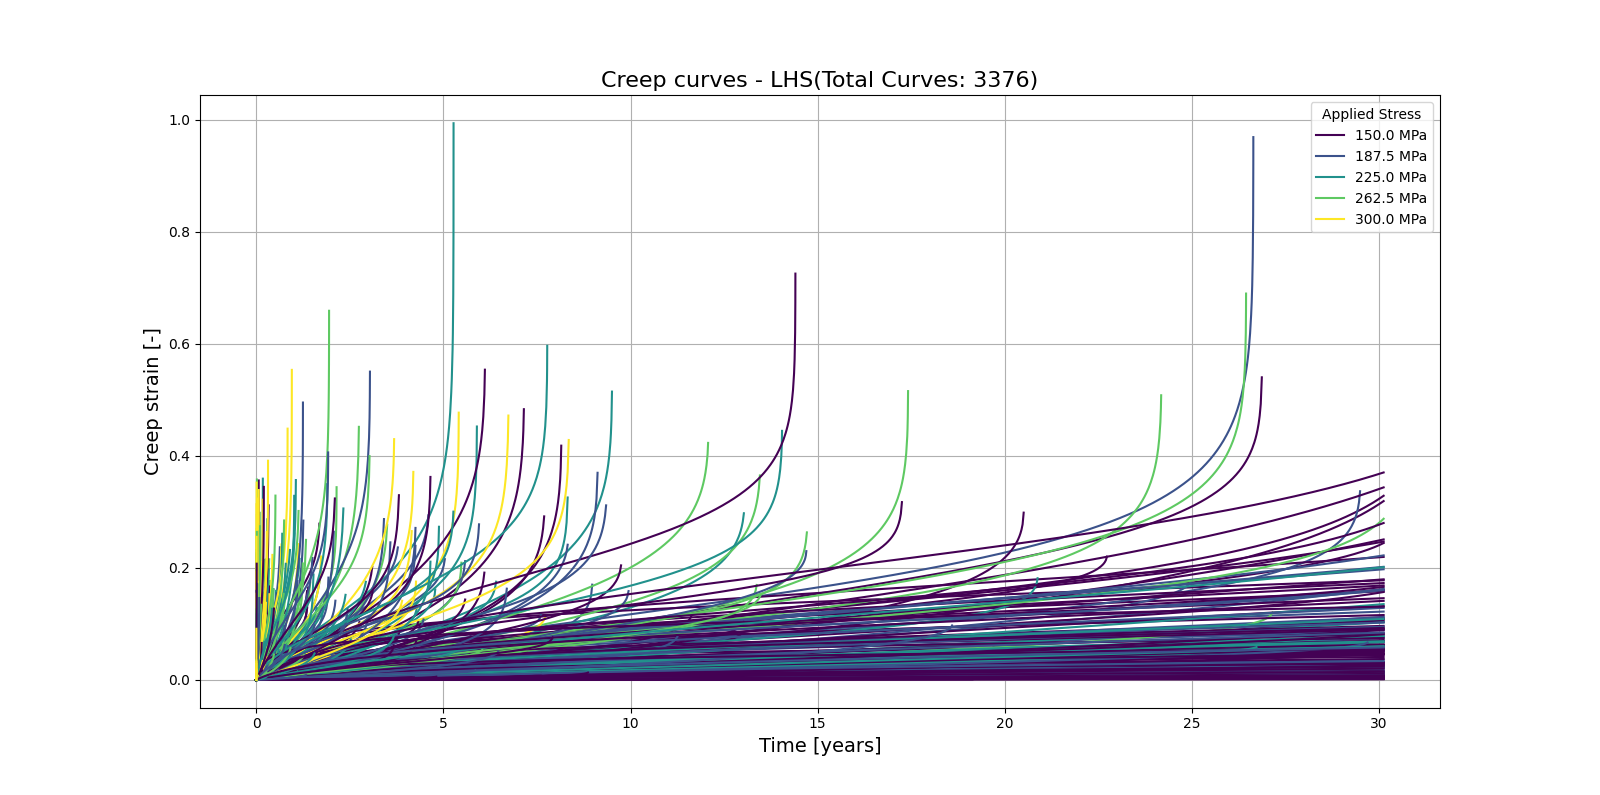
\includegraphics[width=1\textwidth]{figures/creep_curves_LHS.png}
		\caption{Ccreep strain-time curves from Lagamine simulations under different stress levels and material parameters.}
		\label{fig:fem_curves}
	\end{figure}

	\section{Creep Curve Representations}
	\label{Section::Results_CreepCurveRepresentations}
	
	\subsection{Empirical Models Curve Representations}
	\label{Subsection::Results_EmpiricalModels}
	
	This section presents the results of fitting the creep curves using the two empirical models described earlier: the $\theta$-projection model and the three-stage exponential creep model [\textit{see Section}~\ref{Subsection::Empirical_Models}].
	
	\subsubsection{1. $\theta$-Projection Model Fit}
	\label{Subsubsection::Results_ThetaProjection}
	
	Each creep curve was fitted using the $\theta$-projection model described in Equation~\ref{eq:theta_projection}.
	
	Figure~\ref{fig:theta_fit_whole_set} shows the original vs. fitted curve colour-coded by the deviation between them. The solid lines represent the fitted curves, while the dashed lines represent the original creep curves.
	
	\begin{figure}[H]
		\centering
		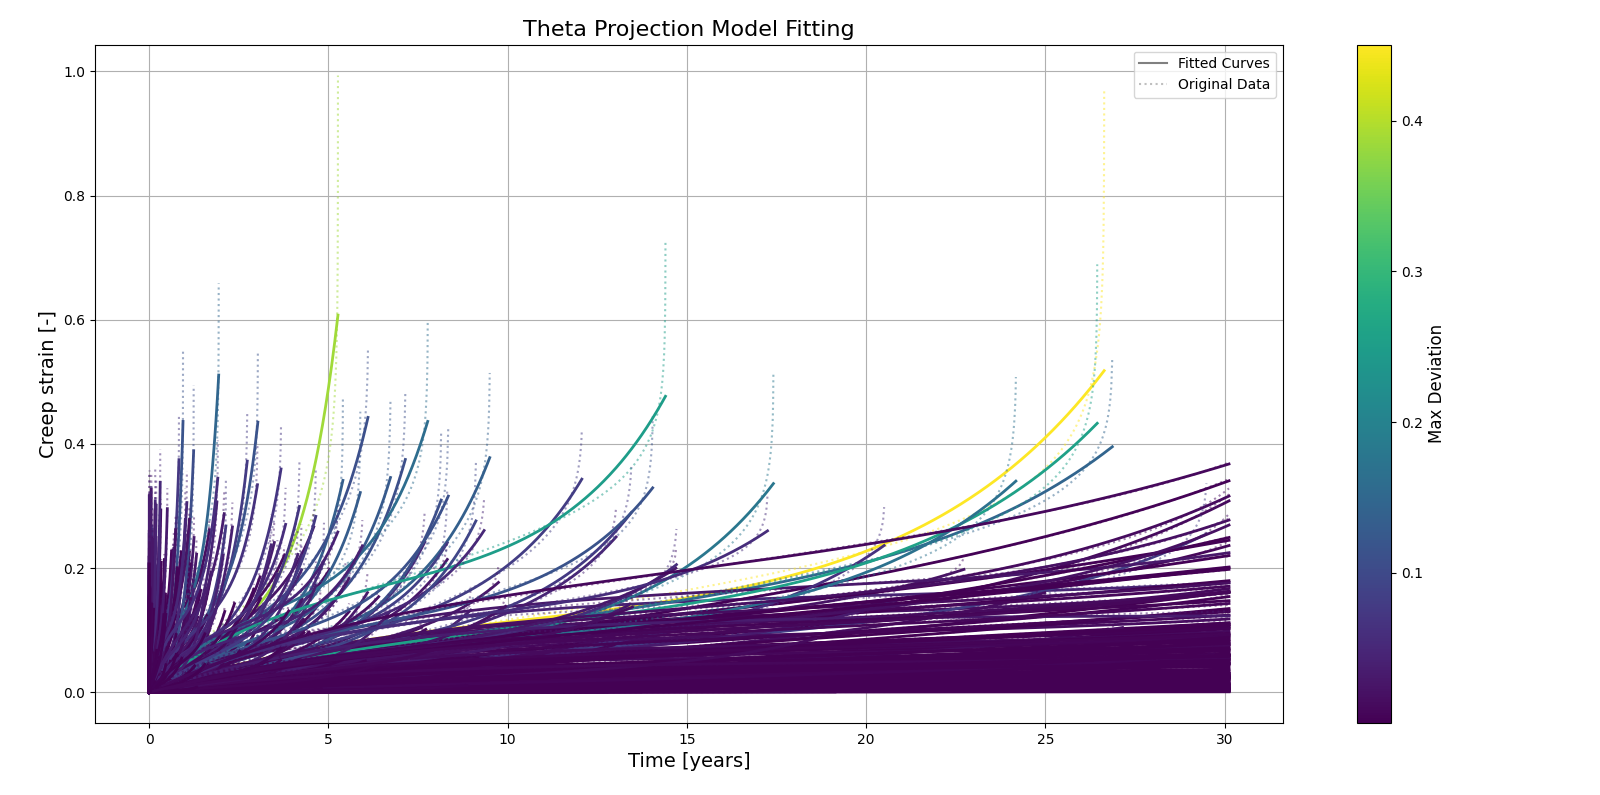
\includegraphics[width=0.95\textwidth]{figures/theta_projection_whole_dataset.png}
		\caption{$\theta$-projection fit by deviation.}
		\label{fig:theta_fit_whole_set}
	\end{figure}
	
	Figure~\ref{fig:theta_fit_max_deviation} shows the creep curve with the largest deviation from its fitted counterpart.
	
	\begin{figure}[H]
		\centering
		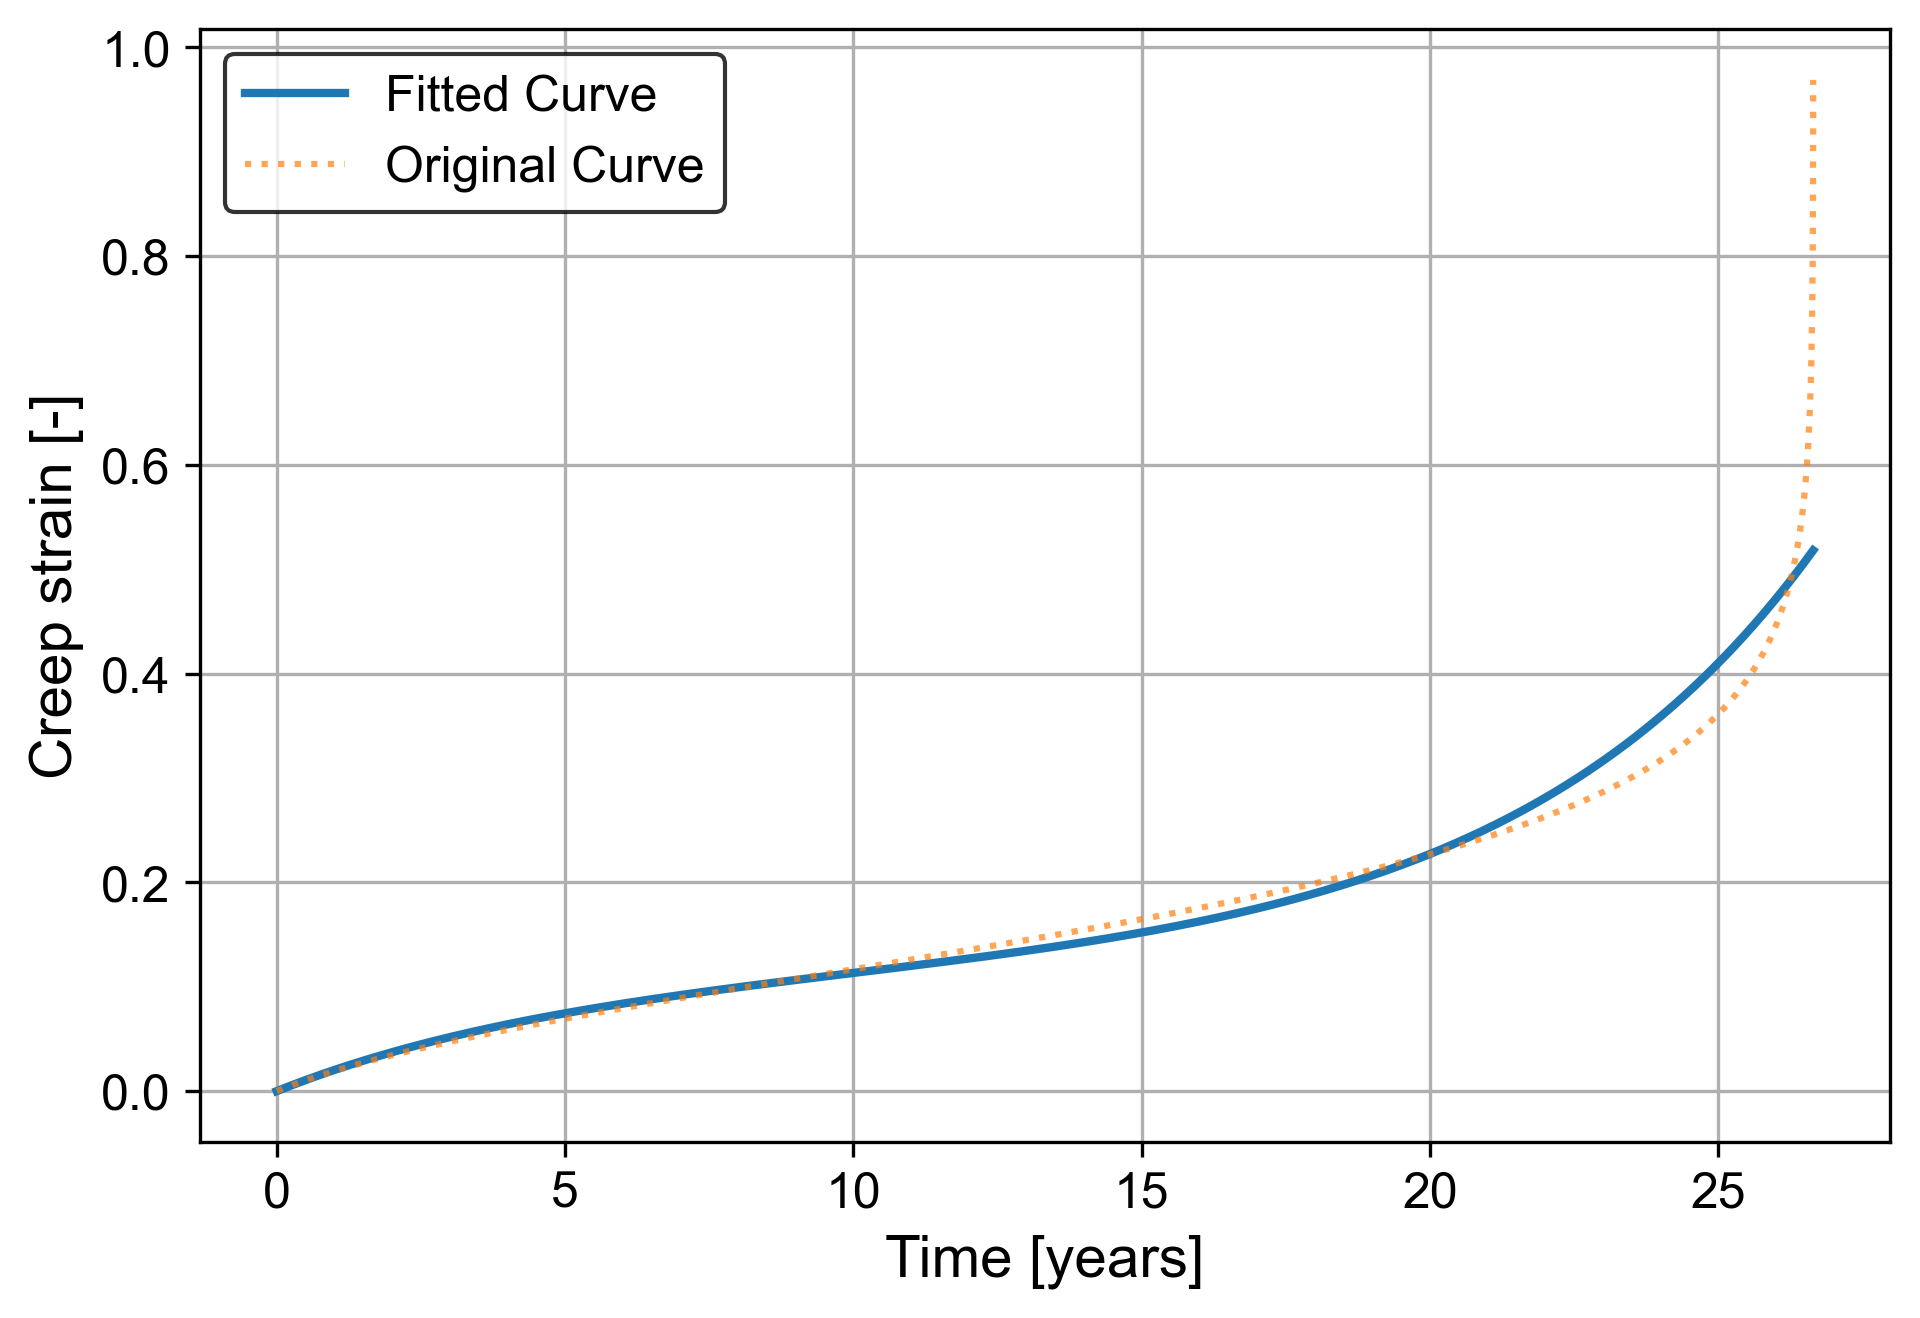
\includegraphics[width=0.85\textwidth]{figures/theta_projection_max_deviation.png}
		\caption{$\theta$-projection fit - Max deviation creep curve.}
		\label{fig:theta_fit_max_deviation}
	\end{figure}
		
	\subsubsection{2. Three Parameter Model Fit}
	\label{Subsubsection::Results_ThreeStage}
	
	The three-parameter exponential model (Equation~\ref{eq:three_stage_creep_equation}) was applied to the same dataset. It provided a continuous representation across all creep phases.
	

	Figure~\ref{fig:three_stage_fit_whole_dataset} shows the original vs. fitted curve colour coded by the deviation. Solid lines represent the fitted curves while the broken lines represent the original creep curves.
	
	\begin{figure}[H]
		\centering
		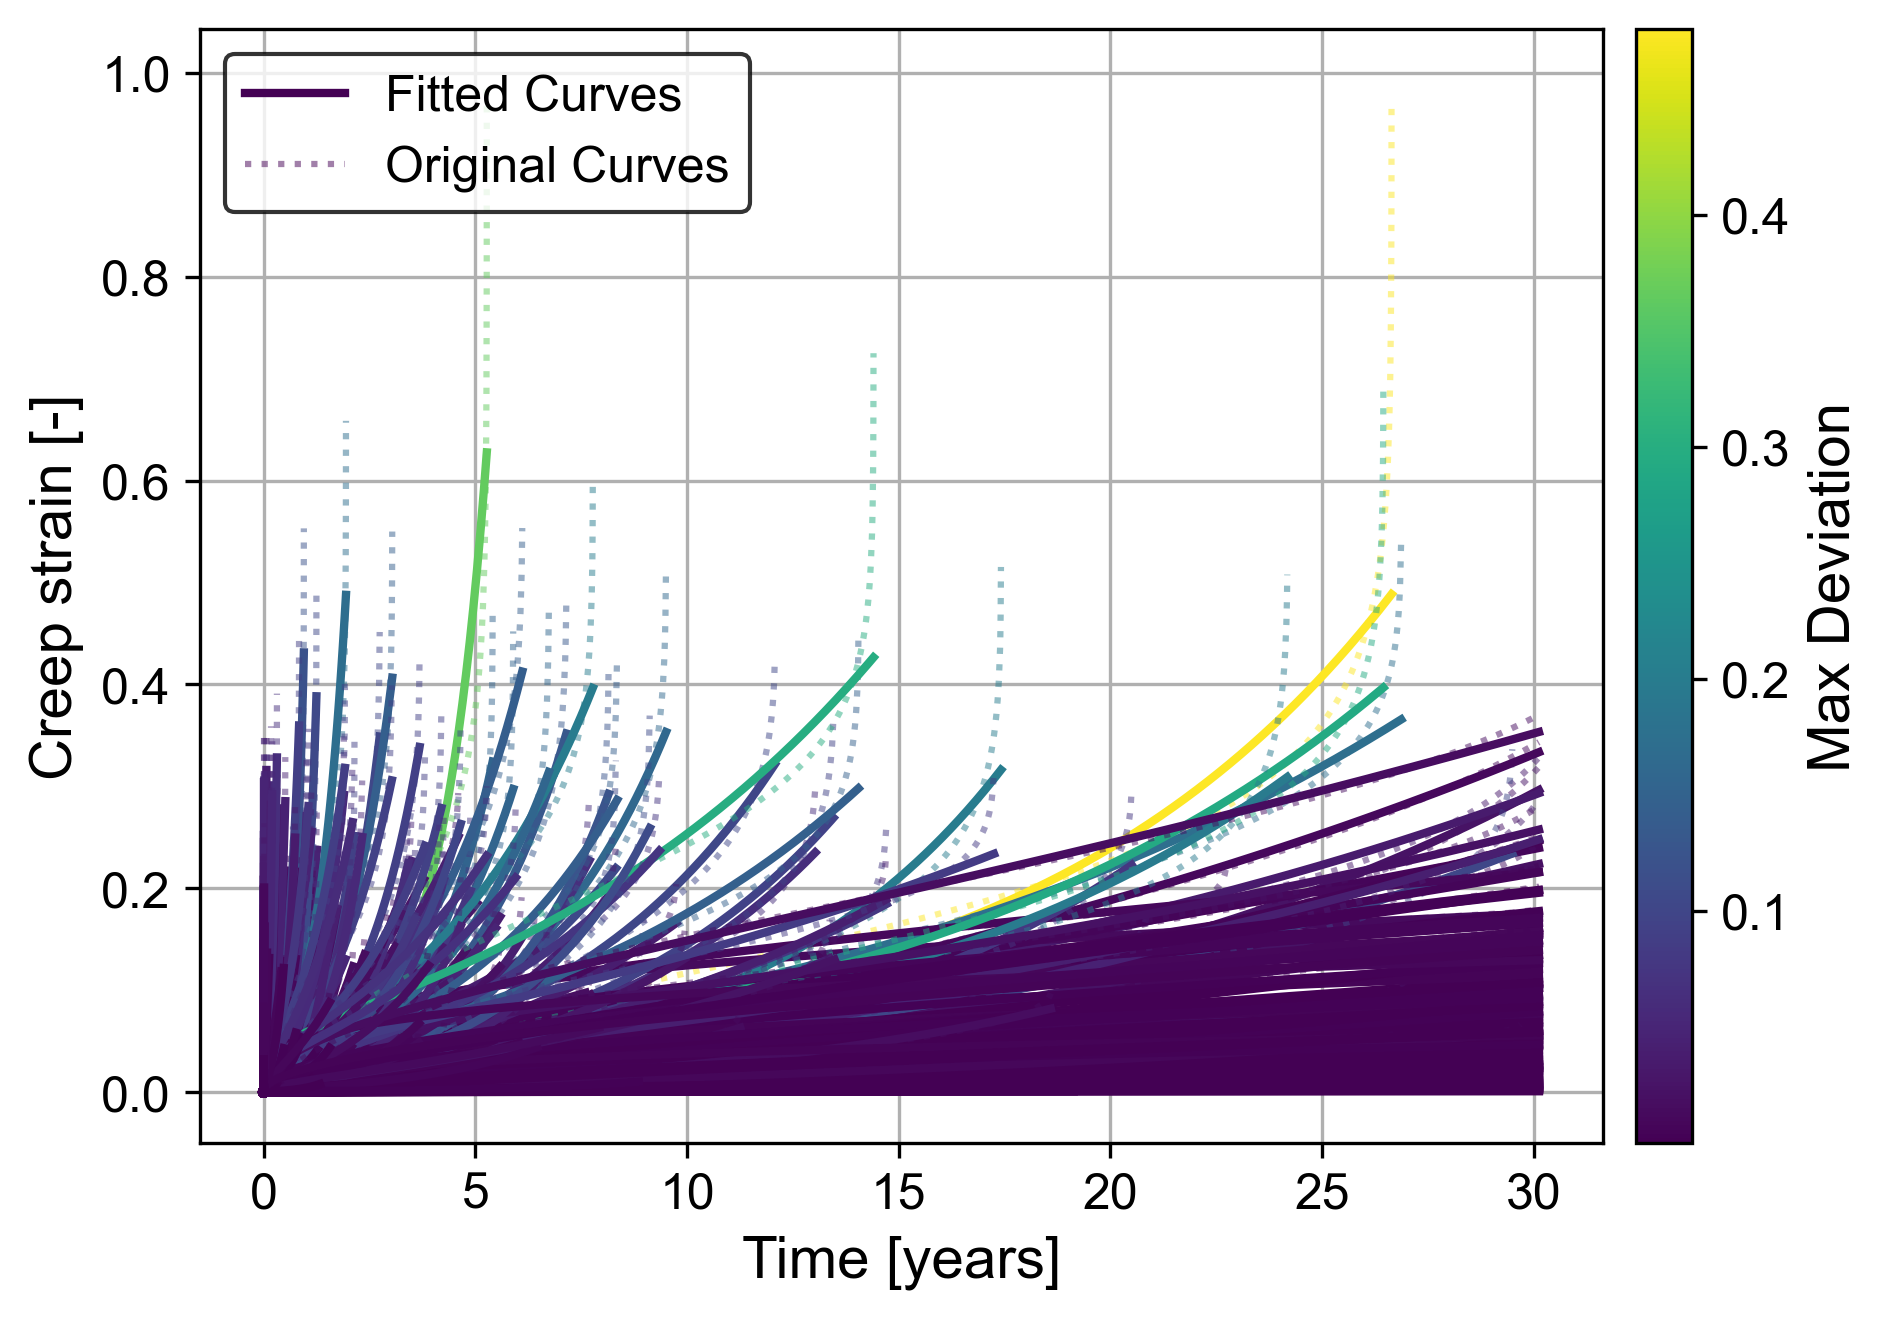
\includegraphics[width=0.95\textwidth]{figures/three_param_model_whole_dataset.png}
		\caption{Three Parameter creep model fit by deviation.}
		\label{fig:three_stage_fit_whole_dataset}
	\end{figure}
	
	Figure~\ref{fig:three_stage_fit_max_deviation} shows the creep curve with the poorest fit from the original.
	
	\begin{figure}[H]
		\centering
		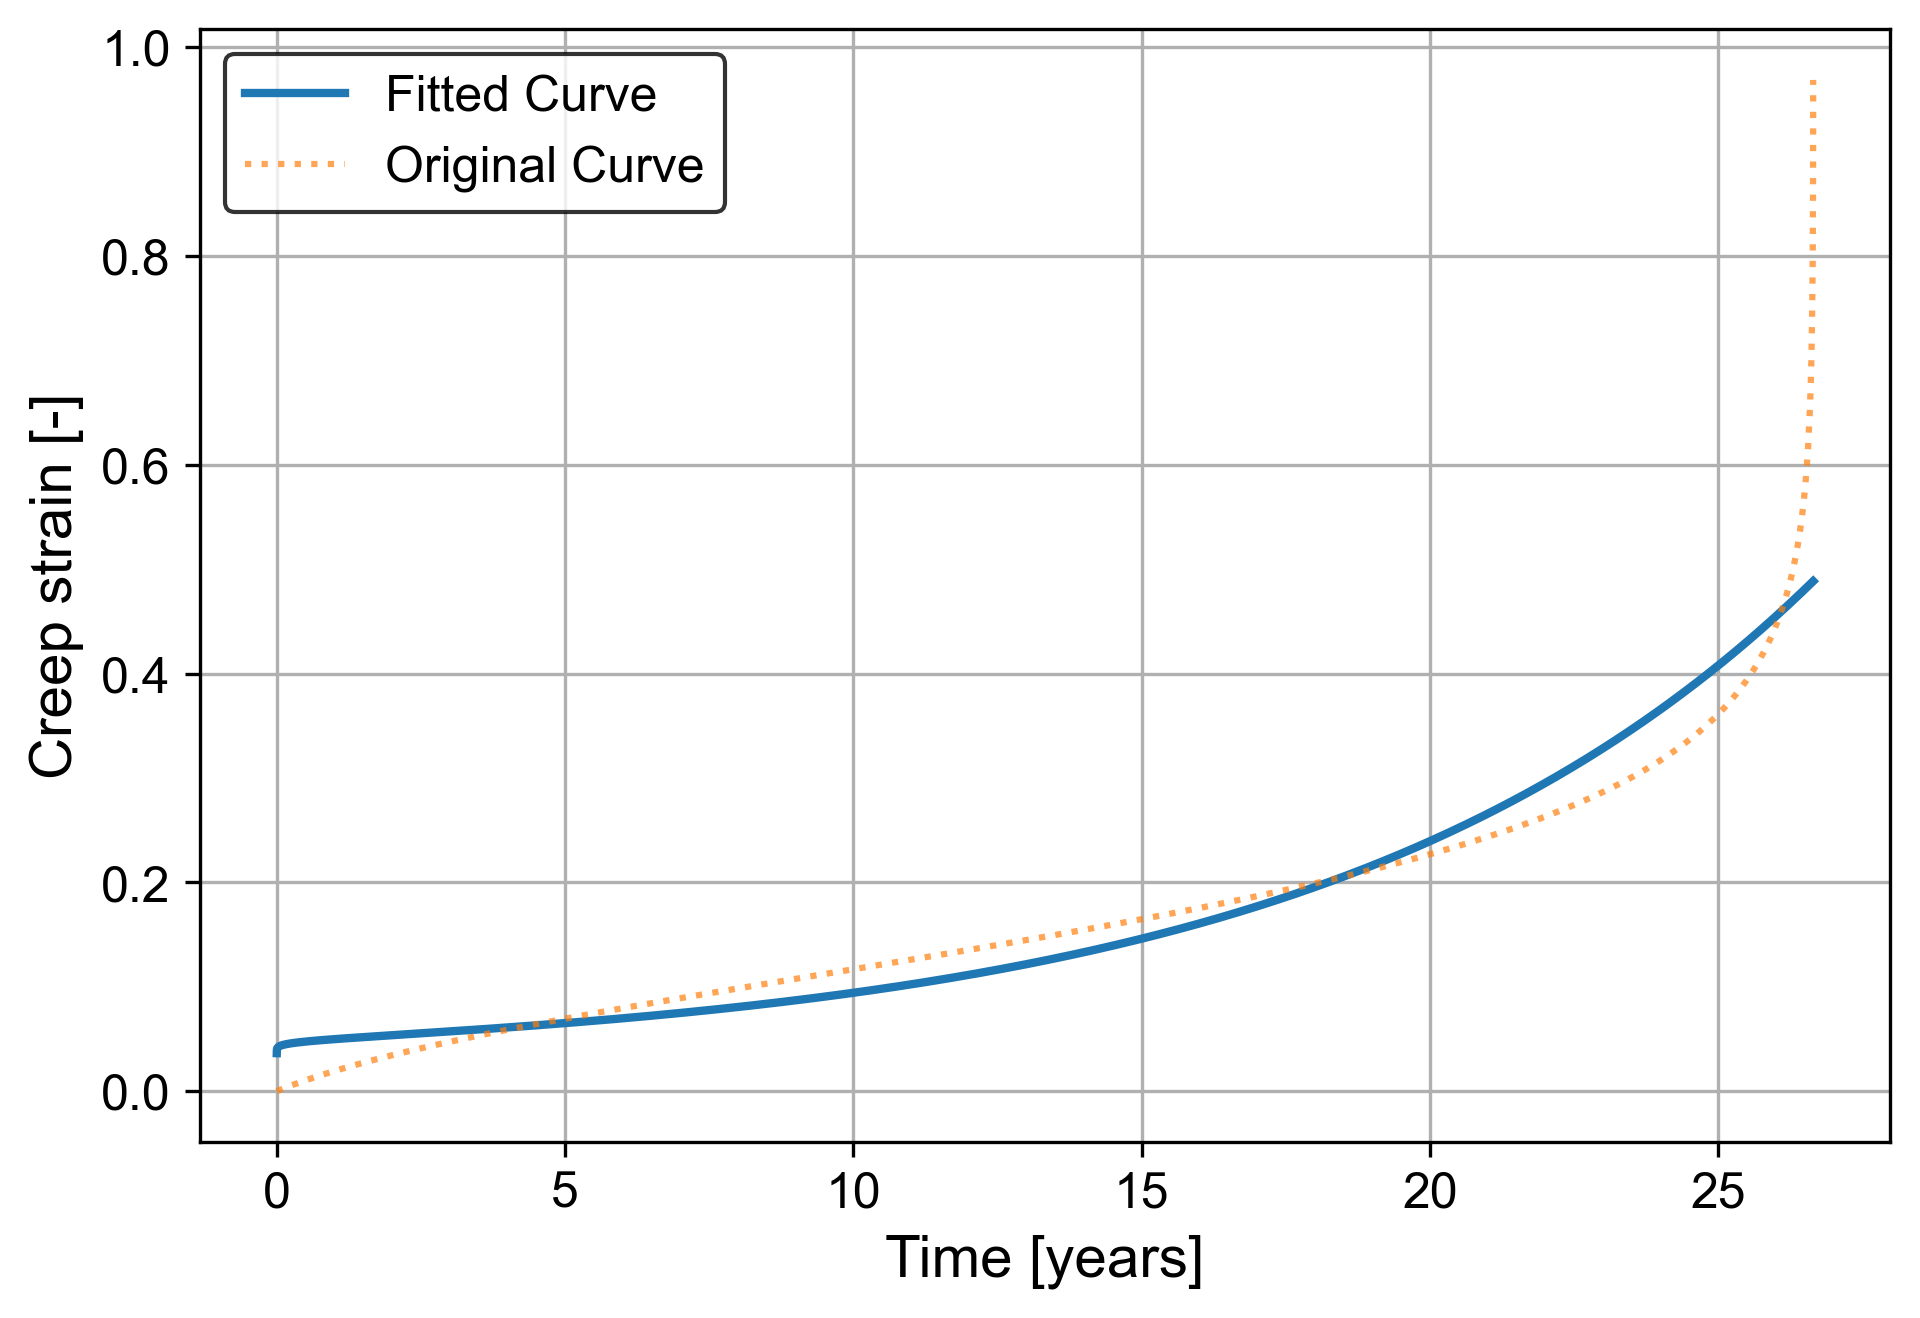
\includegraphics[width=0.85\textwidth]{figures/three_param_model_max_deviation.png}
		\caption{$\theta$-projection fit - Max deviation creep curve.}
		\label{fig:three_stage_fit_max_deviation}
	\end{figure}
	
	\subsection{Data-Driven Models}
	\label{Subsection::Results_DataDrivenModels}
	
	\subsubsection{1. Principal Component Analysis (PCA)}
	
	PCA was applied to the preprocessed creep strain-time data. The three strategies to handle the different input vector lengths had different results. For visualization, 6 random curves from the test set are plotted with the original creep curve against the reconstructed creep curve. This is done for all the three strategies. 
	
	\subsubsubsection{Zero Padding:}
	
	The variance captured by each principal component is summarized in Figure~\ref{fig:pca_variance_zero}.
	
	\begin{figure}[H]
		\centering
		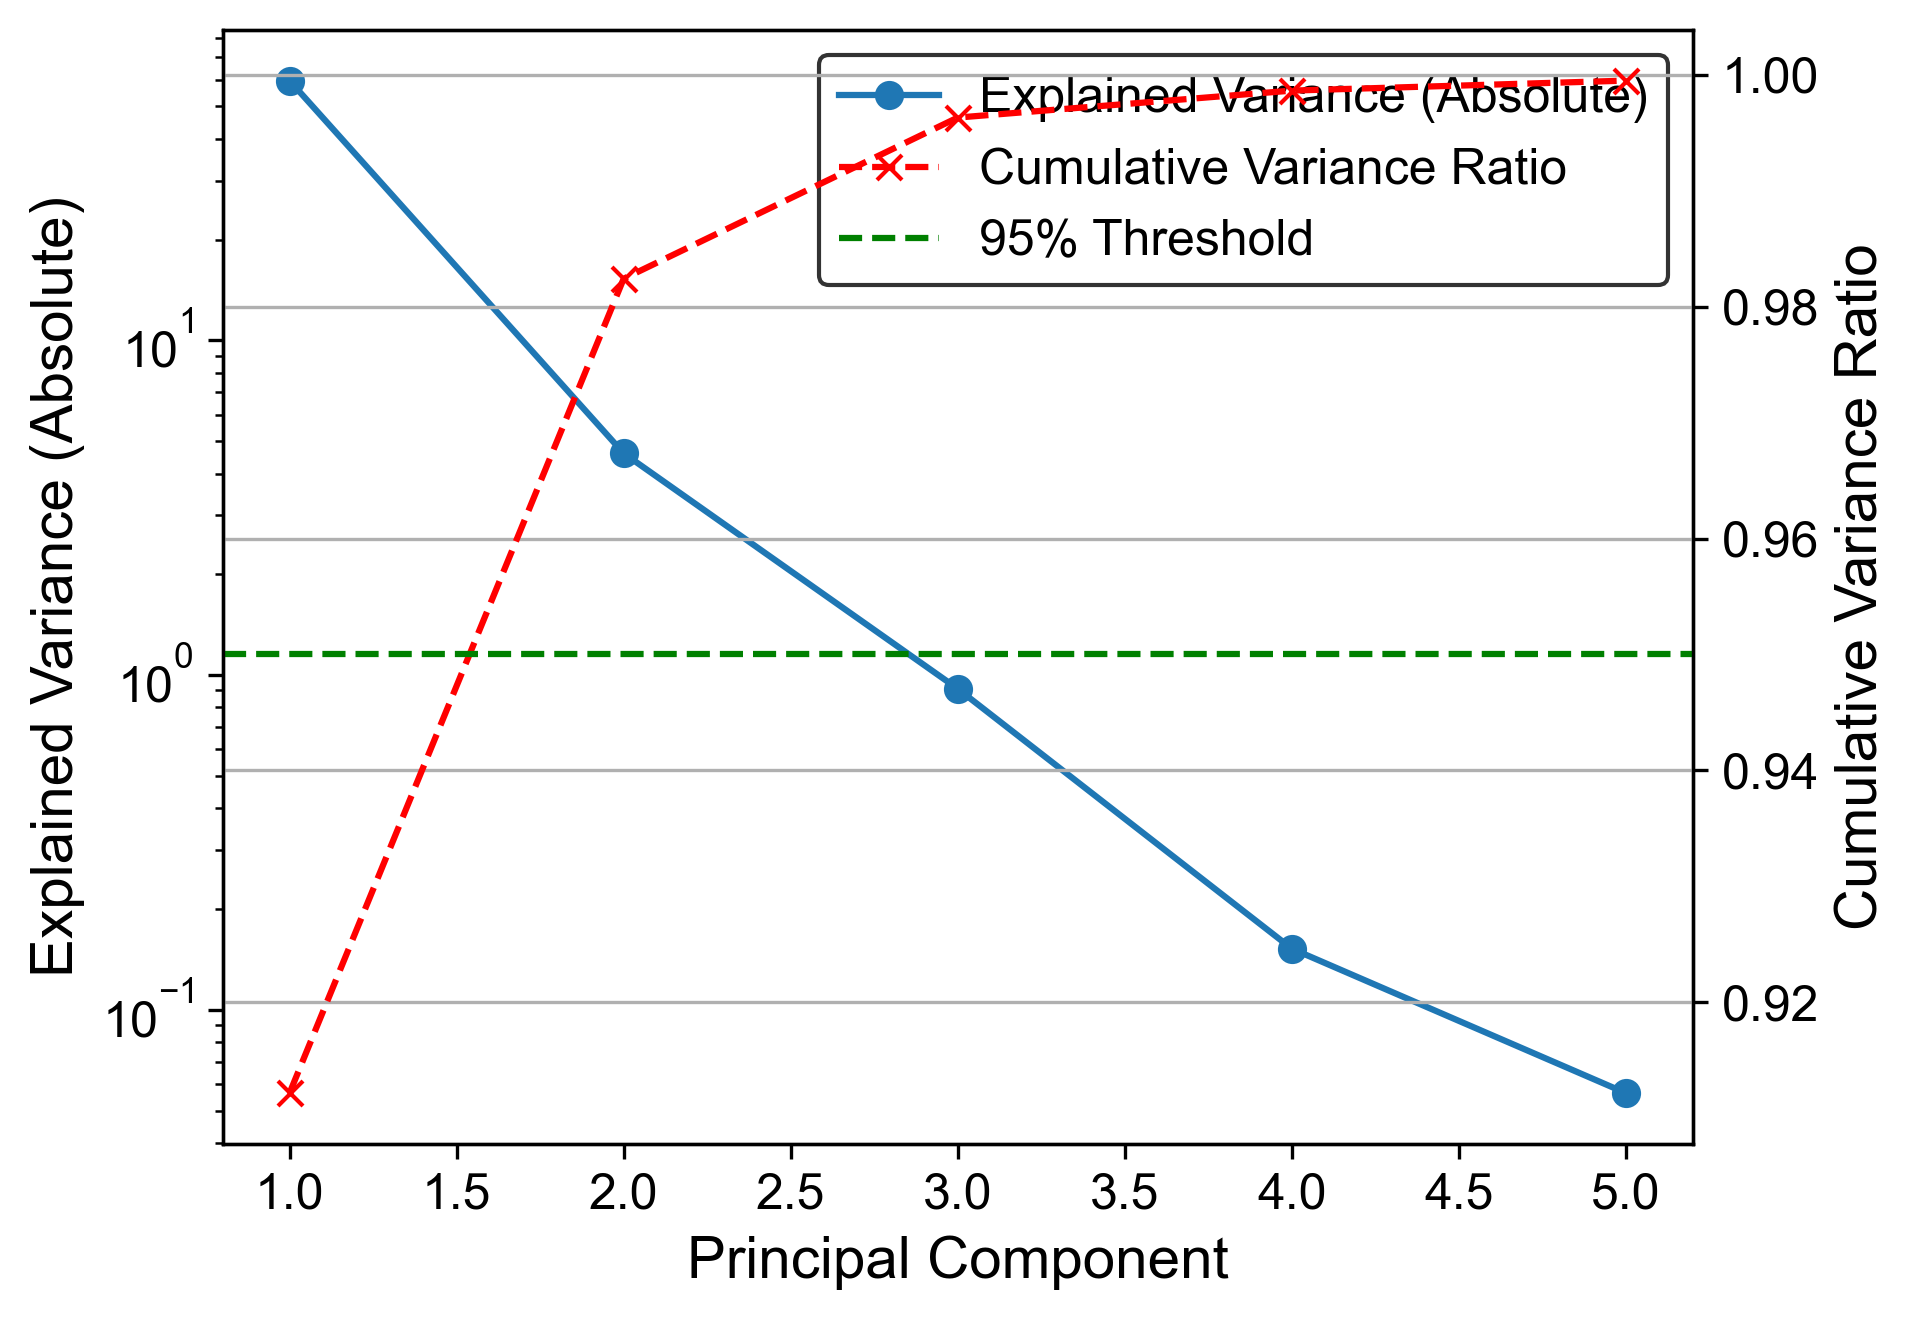
\includegraphics[width=0.65\textwidth]{figures/pca_var_zero_fill.png}
		\caption{Explained variance by each principal component (PCA).}
		\label{fig:pca_variance_zero}
	\end{figure}
	
	The first 2 components captured over 95\% of the total variance.	
	
	The original vs. the reconstructed creep curves with zero padding is shown in figure~\ref{fig:pca_zero_fill}.
	
	\begin{figure}[H]
		\centering
		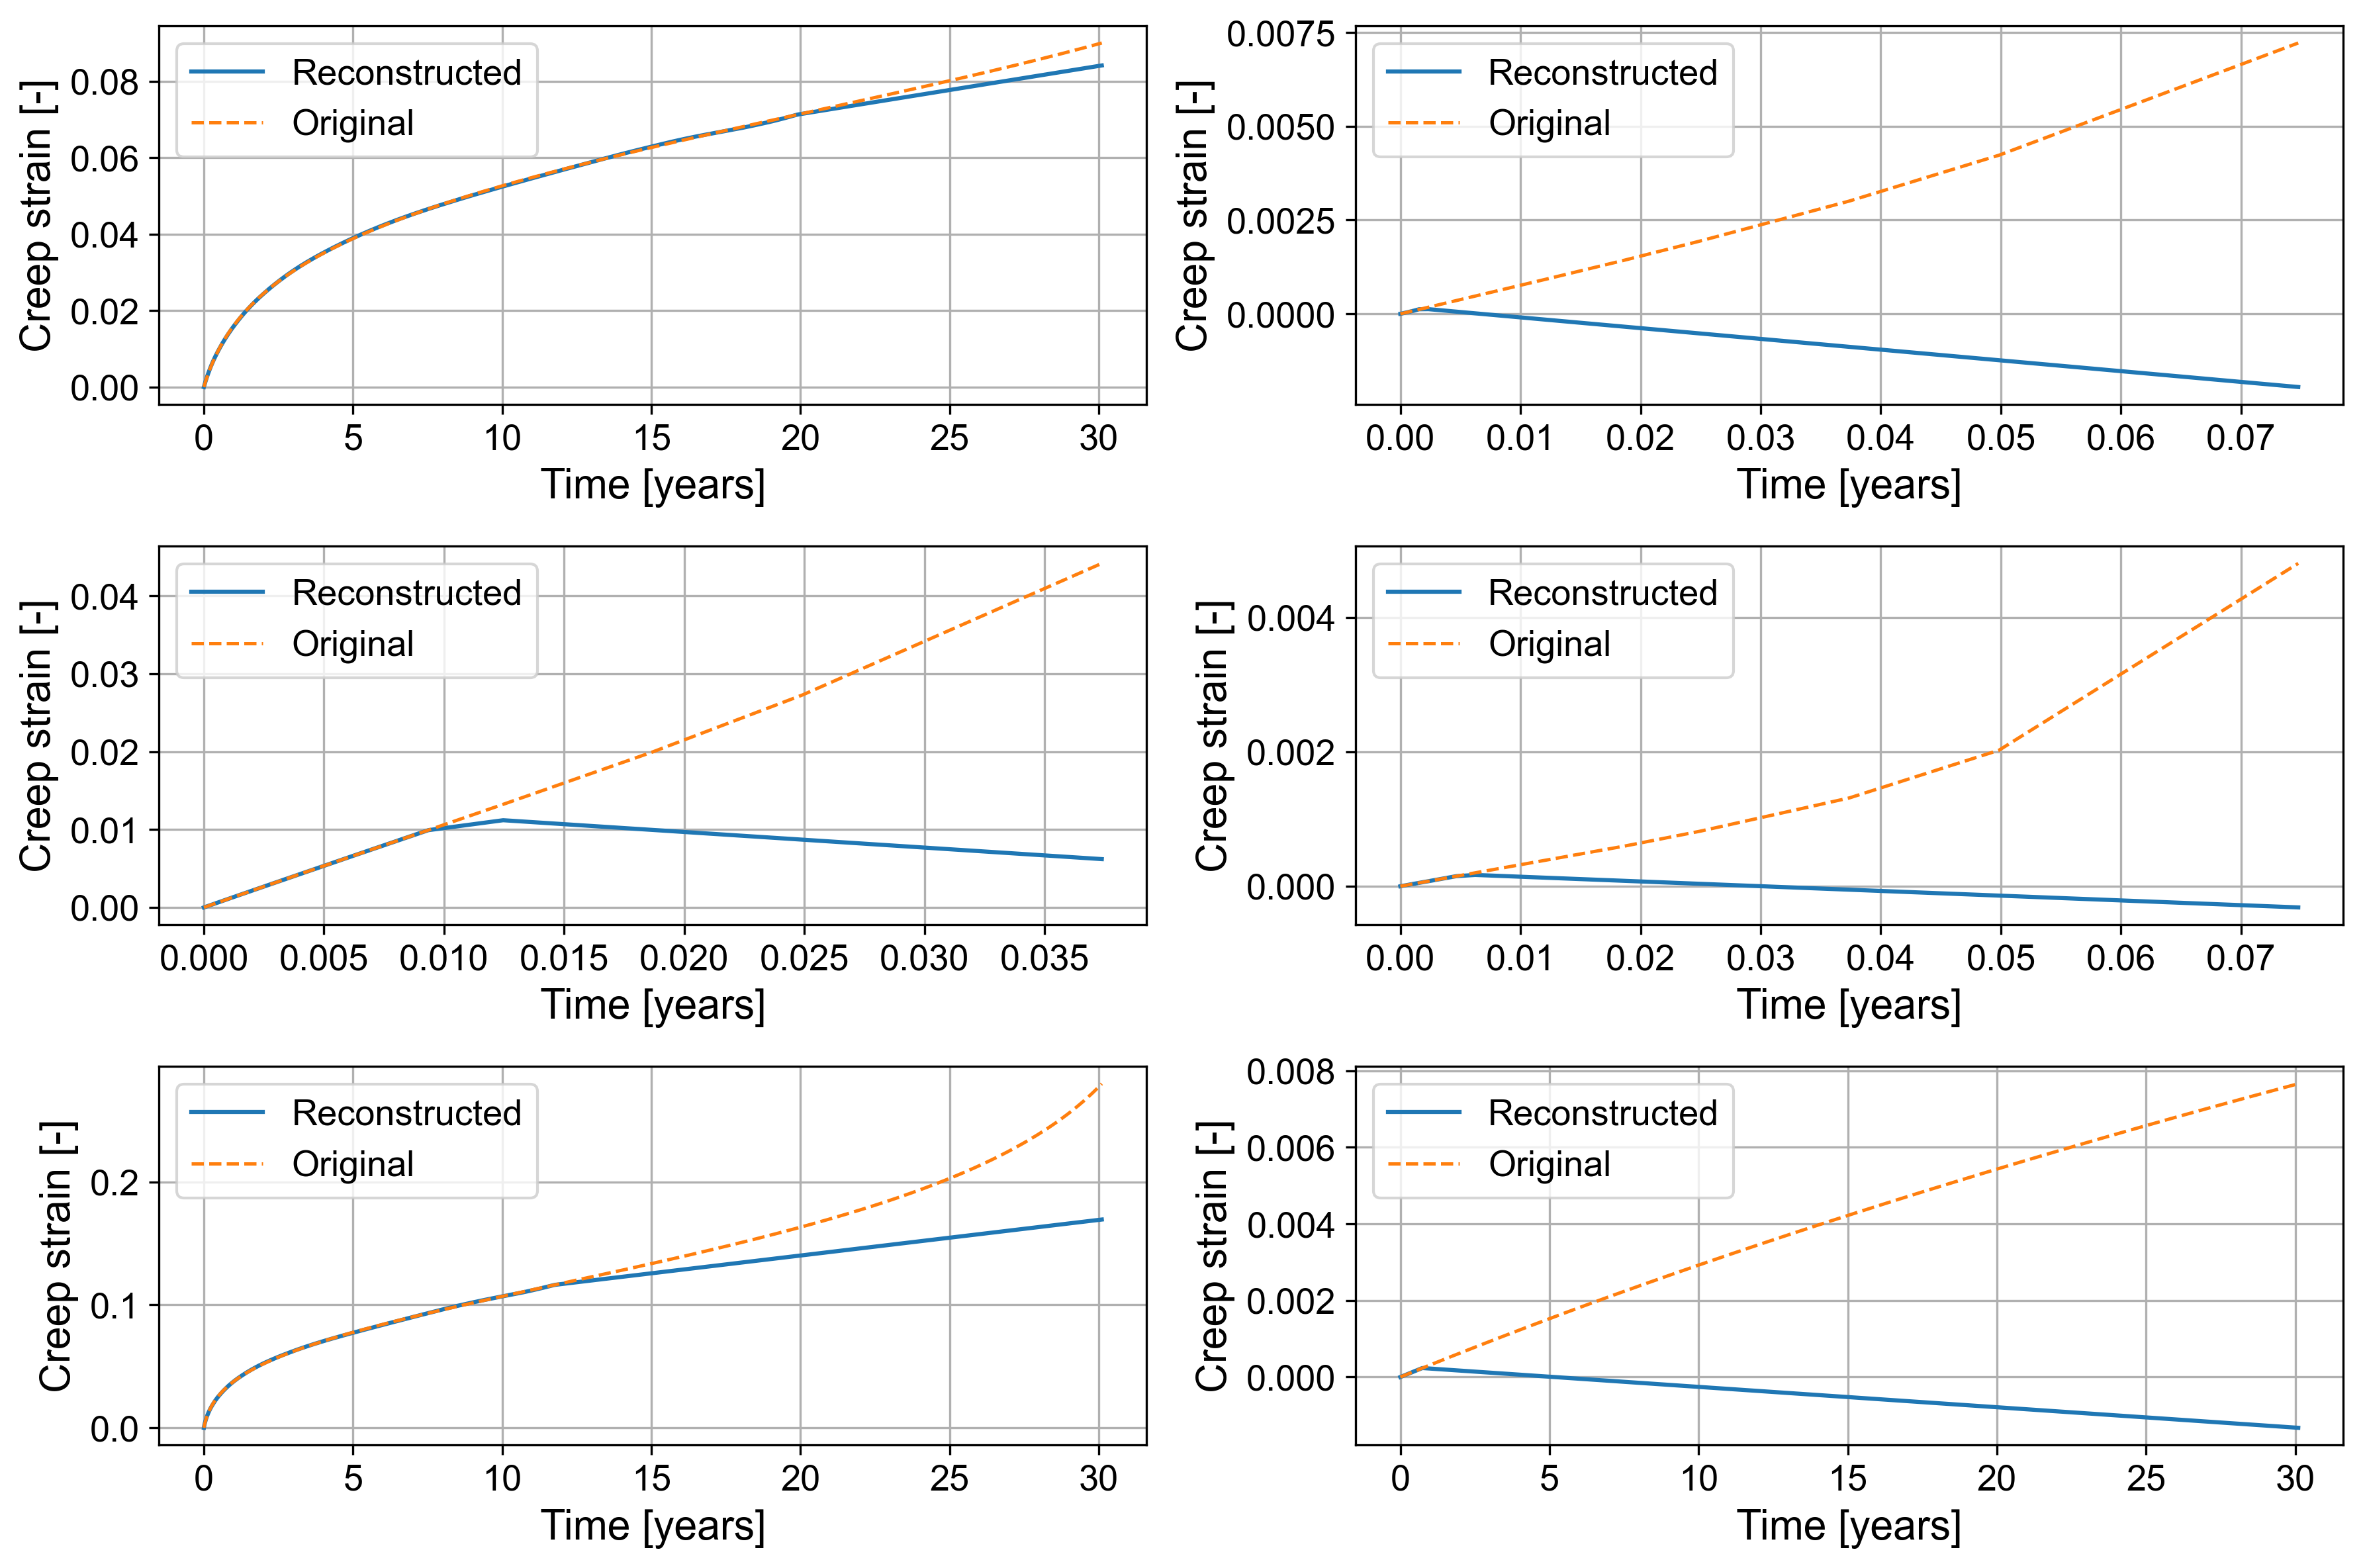
\includegraphics[width=1\textwidth]{figures/pca_reconstructed_curves_zero_fill.png}
		\caption{Original vs. Reconstructed Creep Curves(PCA) - Zero paddding.}
		\label{fig:pca_zero_fill}
	\end{figure}
	
	\subsubsubsection{Max Creep Strain Padding:}
	
	The variance captured by each principal component is summarized in Figure~\ref{fig:pca_variance_max}.
	
	\begin{figure}[H]
		\centering
		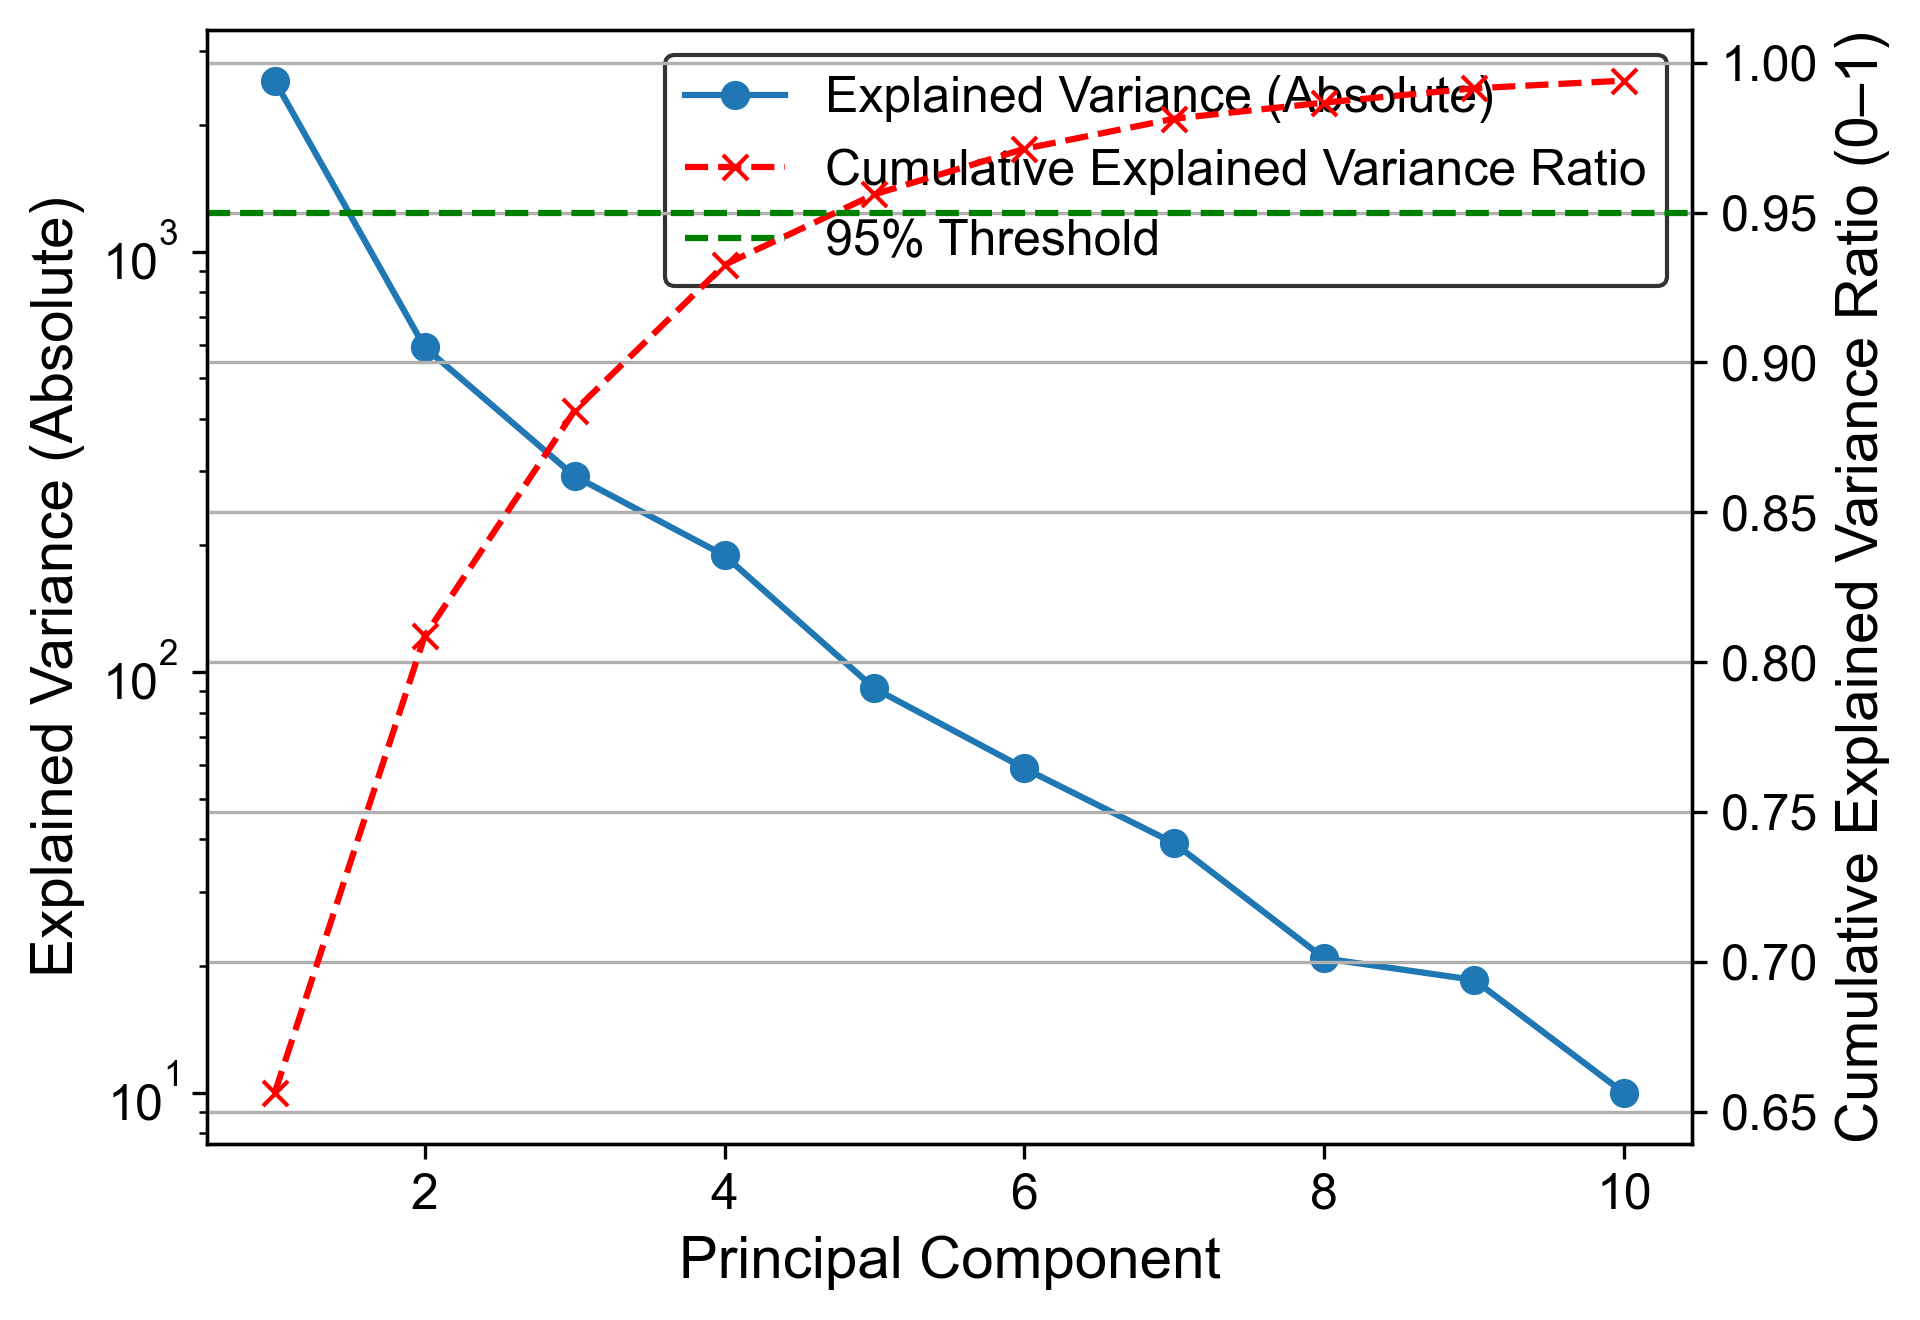
\includegraphics[width=0.65\textwidth]{figures/pca_var_max_fill.png}
		\caption{Explained variance by each principal component (PCA).}
		\label{fig:pca_variance_max}
	\end{figure}
	
	The first 5 components captured over 95\% of the total variance.	
	
	The original vs. the reconstructed creep curves with the maximum creep strain padding is shown in figure~\ref{fig:pca_max_fill}.
	
	\begin{figure}[H]
		\centering
		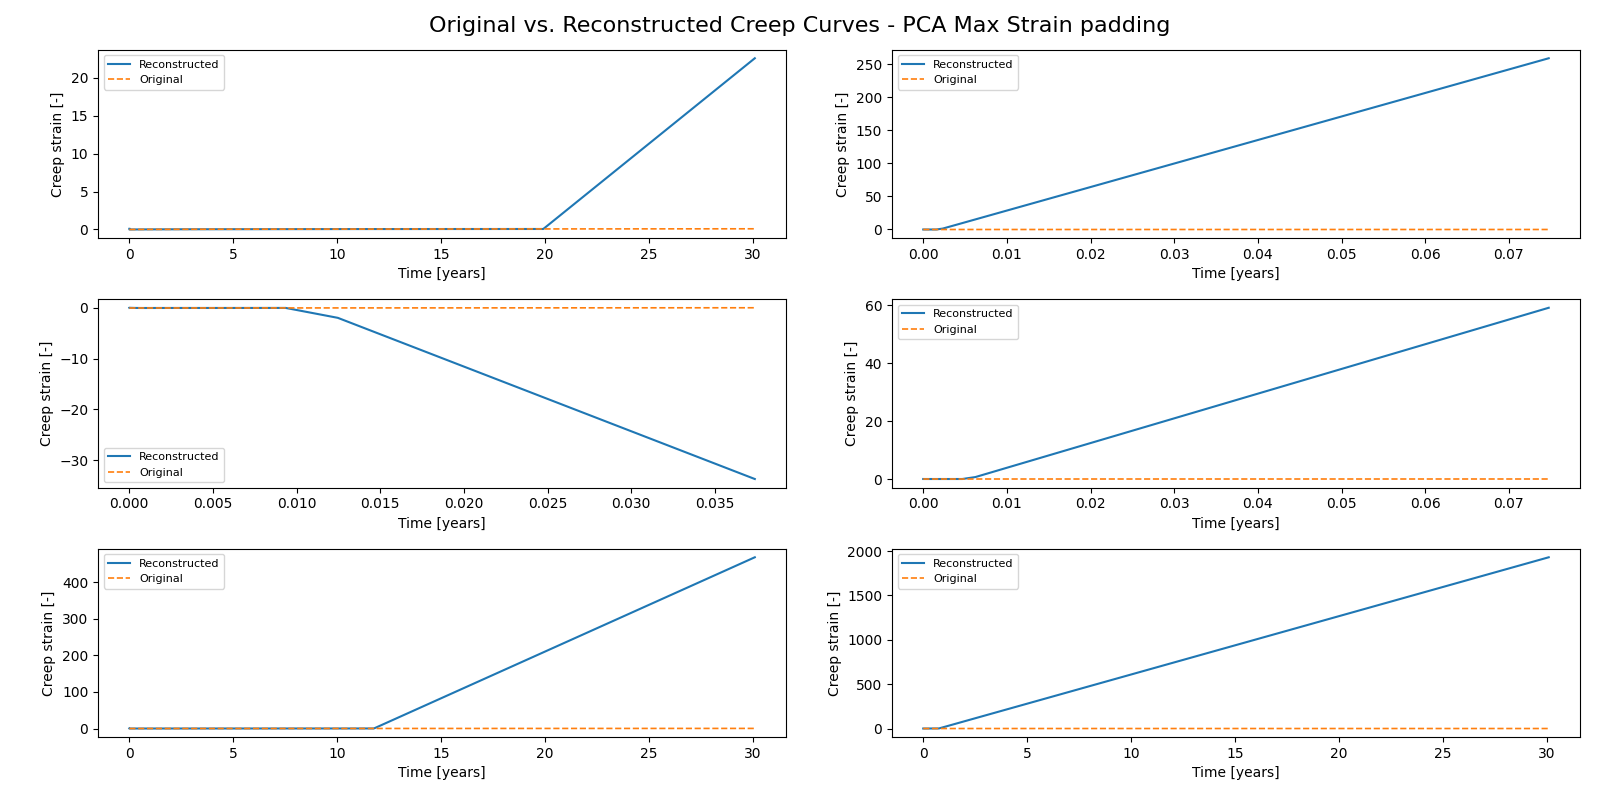
\includegraphics[width=1\textwidth]{figures/pca_reconstructed_curves_max_fill.png}
		\caption{Original vs. Reconstructed Creep Curves(PCA) - Max creep strain paddding.}
		\label{fig:pca_max_fill}
	\end{figure}
	
	\subsubsubsection{Normalization by Rupture time:}
	
	The variance captured by each principal component is summarized in Figure~\ref{fig:pca_variance_norm}.
	
	\begin{figure}[H]
		\centering
		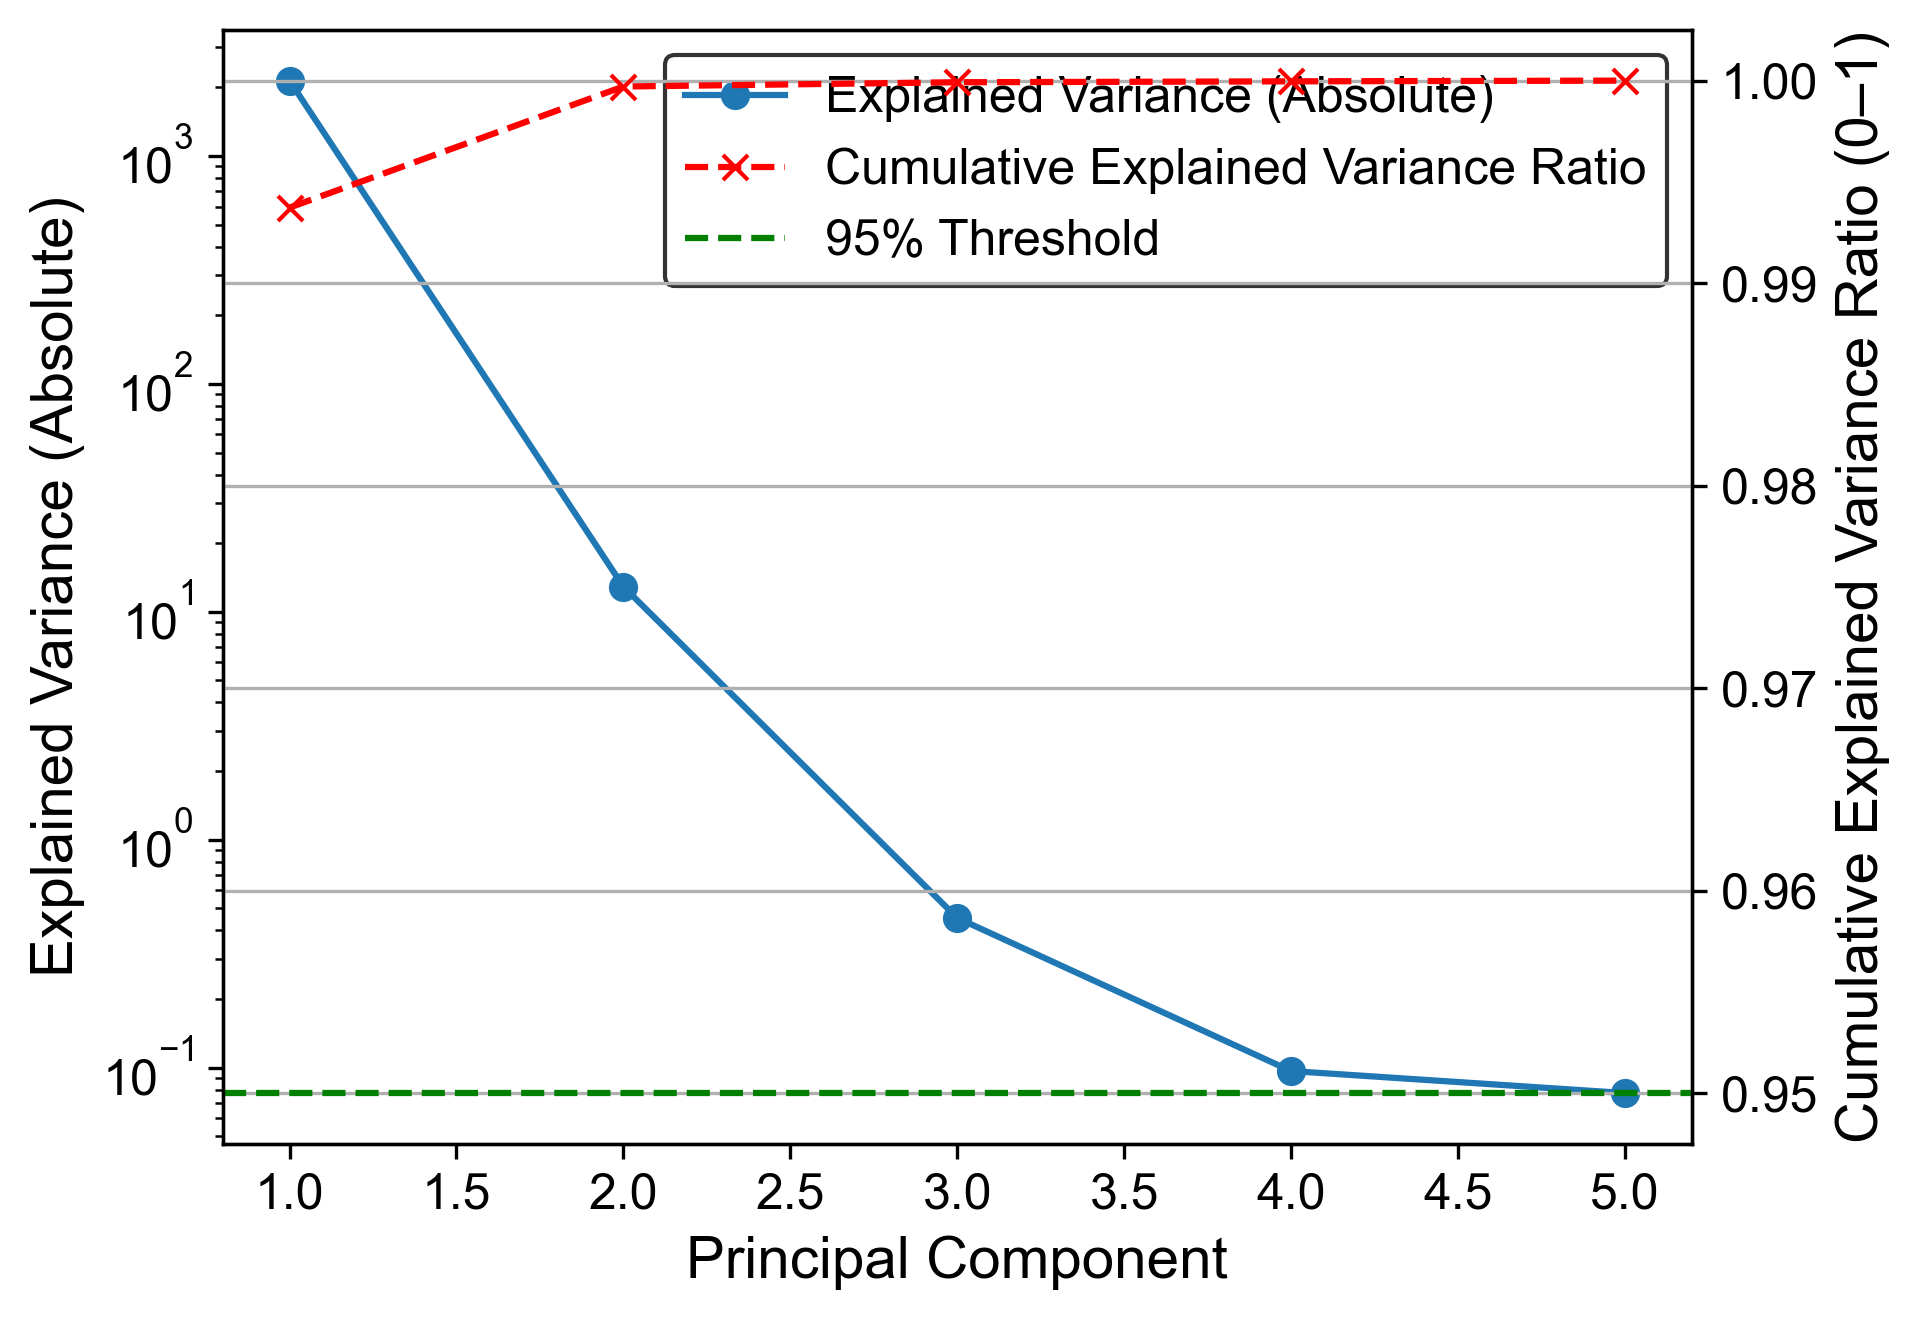
\includegraphics[width=0.65\textwidth]{figures/pca_var_norm.png}
		\caption{Explained variance by each principal component (PCA).}
		\label{fig:pca_variance_norm}
	\end{figure}
	
	The first component captured over 95\% of the total variance.	
	
	The original vs. the reconstructed creep curves with the normalization by rupture time approach is shown in figure~\ref{fig:pca_norm_rupture_time}.
	
	\begin{figure}[H]
		\centering
		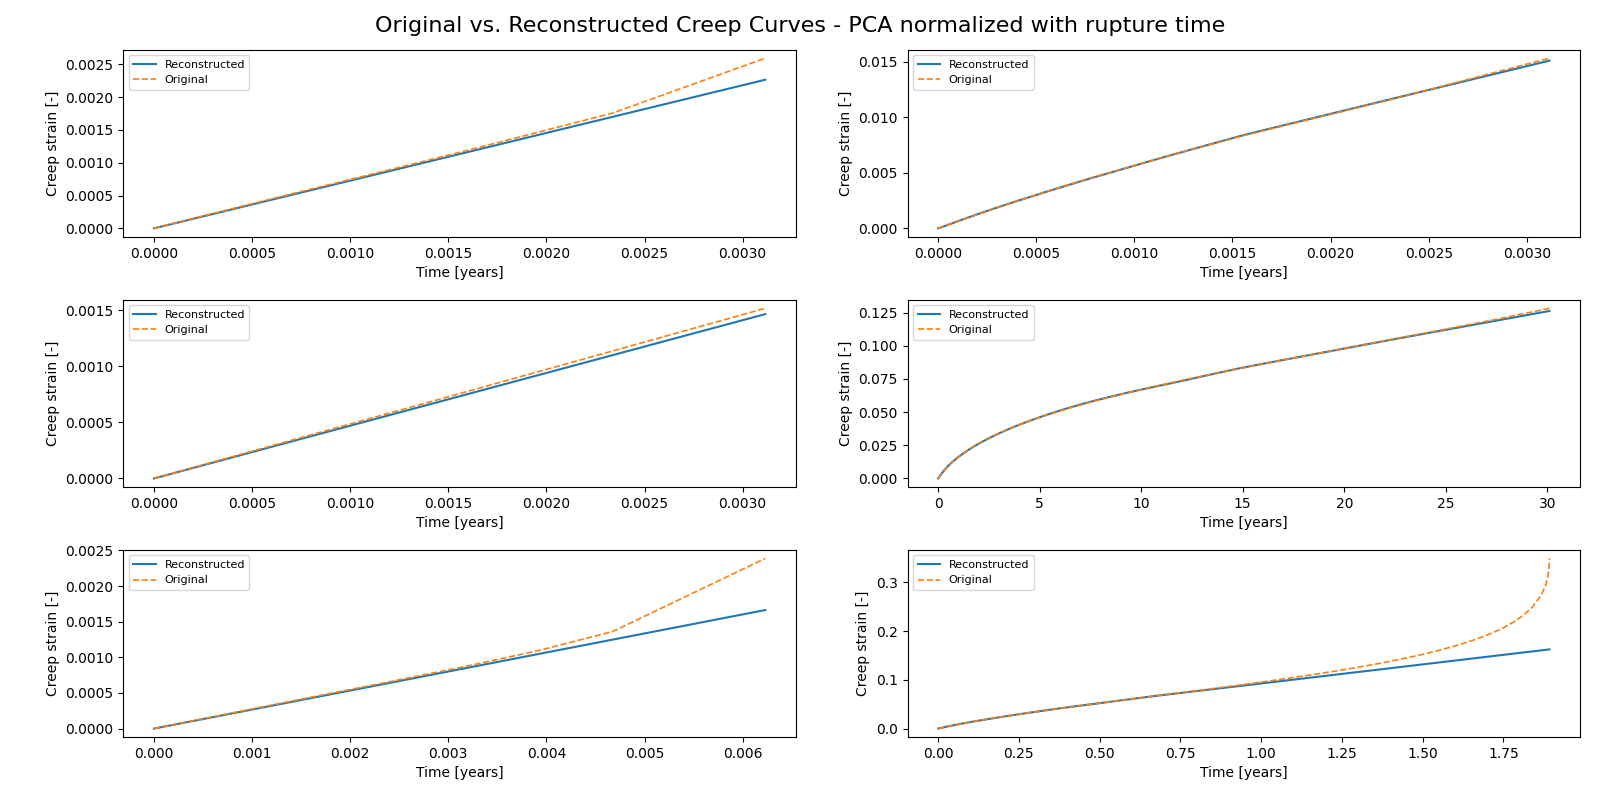
\includegraphics[width=1\textwidth]{figures/pca_reconstructed_curves_norm.png}
		\caption{Original vs. Reconstructed Creep Curves(PCA) - Normalization by rupture time approach.}
		\label{fig:pca_norm_rupture_time}
	\end{figure}
	
	\subsubsection{2. Kernel PCA (KPCA)}
	
	Kernel PCA using polynomial and RBF kernels to the preprocessed creep strain-time data. Similar to PCA, KPCA shows different results for the different data preprocessing approaches. 
	
	\subsubsubsection{Zero Padding:}
	
	\begin{table}[ht]
		\centering
		\caption{Best parameters for RBF and Polynomial kernels - Zero padding}
		\begin{tabular}{|l|l|l|}
			\hline
			\textbf{Kernel} & \textbf{Best Parameters} \\
			\hline
			RBF & $\{n\_components = 20,\ \gamma = 0.1\}$ \\
			Poly & $\{n\_components = 50,\ \text{degree} = 2,\ \gamma = 0.01,\ \text{coef}_0 = 1\}$  \\
			\hline
		\end{tabular}
		\label{tab:best_params_zero_fill}
	\end{table}
	
	The original vs. the reconstructed creep curves with zero padding is shown in figure~\ref{fig:kpca_zero_fill}.
	
	\begin{figure}[H]
		\centering
		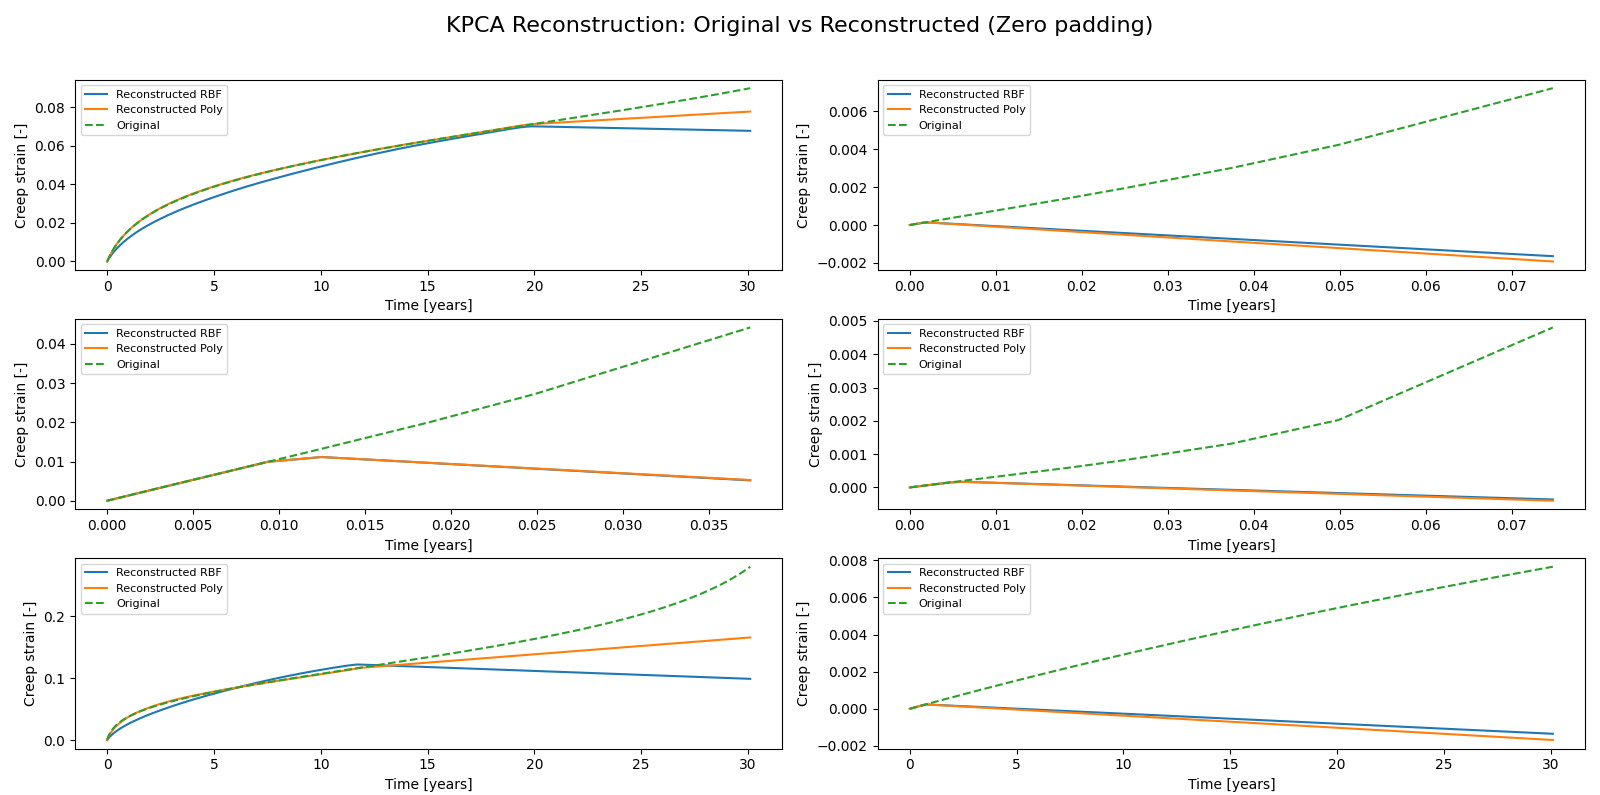
\includegraphics[width=1\textwidth]{figures/kpca_reconstructed_curves_zero_fill.png}
		\caption{Original vs. Reconstructed Creep Curves(KPCA) - Zero paddding.}
		\label{fig:kpca_zero_fill}
	\end{figure}
	
	\subsubsubsection{Max Creep Strain Padding:}
	
	\begin{table}[ht]
		\centering
		\caption{Best parameters for RBF and Polynomial kernels - Max strain padding}
		\begin{tabular}{|l|l|l|}
			\hline
			\textbf{Kernel} & \textbf{Best Parameters} \\
			\hline
			RBF & $\{n\_components = 50,\ \gamma = 0.01\}$ \\
			Poly & $\{n\_components = 50,\ \text{degree} = 3,\ \gamma = 0.001,\ \text{coef}_0 = 1\}$  \\
			\hline
		\end{tabular}
		\label{tab:best_params_max_fill}
	\end{table}
	
	The original vs. the reconstructed creep curves with the maximum creep strain padding is shown in figure~\ref{fig:kpca_max_fill}.
	
	\begin{figure}[H]
		\centering
		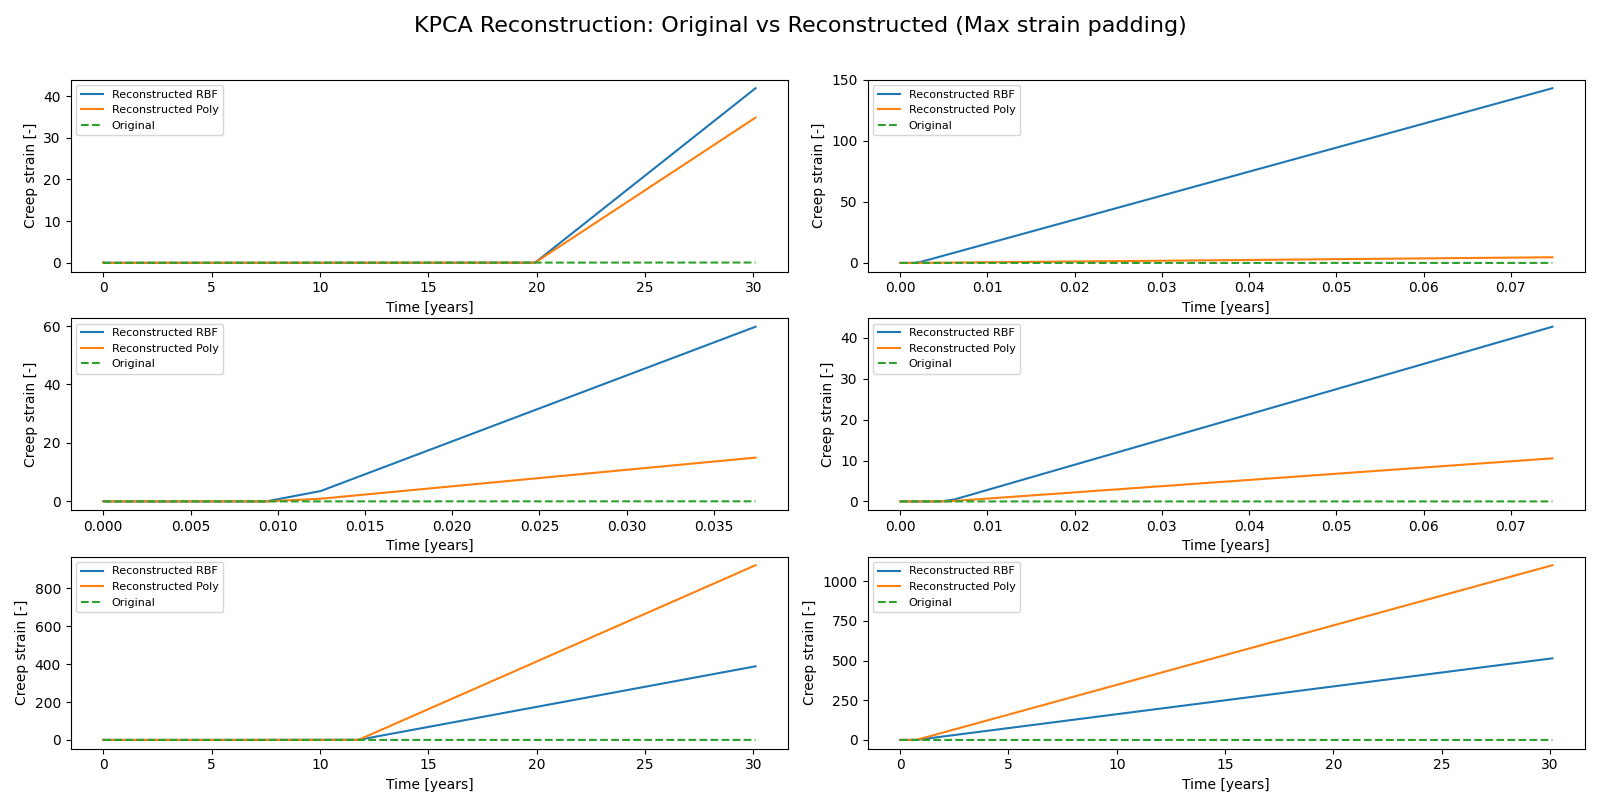
\includegraphics[width=1\textwidth]{figures/kpca_reconstructed_curves_max_fill.png}
		\caption{Original vs. Reconstructed Creep Curves(KPCA) - Max creep strain paddding.}
		\label{fig:kpca_max_fill}
	\end{figure}
	
	\subsubsubsection{Normalization by Rupture time:}
	
	\begin{table}[ht]
		\centering
		\caption{Best parameters for RBF and Polynomial kernels - Normalization by rupture time}
		\begin{tabular}{|l|l|l|}
			\hline
			\textbf{Kernel} & \textbf{Best Parameters} \\
			\hline
			RBF & $\{n\_components = 50,\ \gamma = 1\}$ \\
			Poly & $\{n\_components = 20,\ \text{degree} = 2,\ \gamma = 0.01,\ \text{coef}_0 = 1\}$  \\
			\hline
		\end{tabular}
		\label{tab:best_params_norm}
	\end{table}
	
	The original vs. the reconstructed creep curves with the normalization by rupture time approach is shown in figure~\ref{fig:kpca_norm_rupture_time}.
	
	\begin{figure}[H]
		\centering
		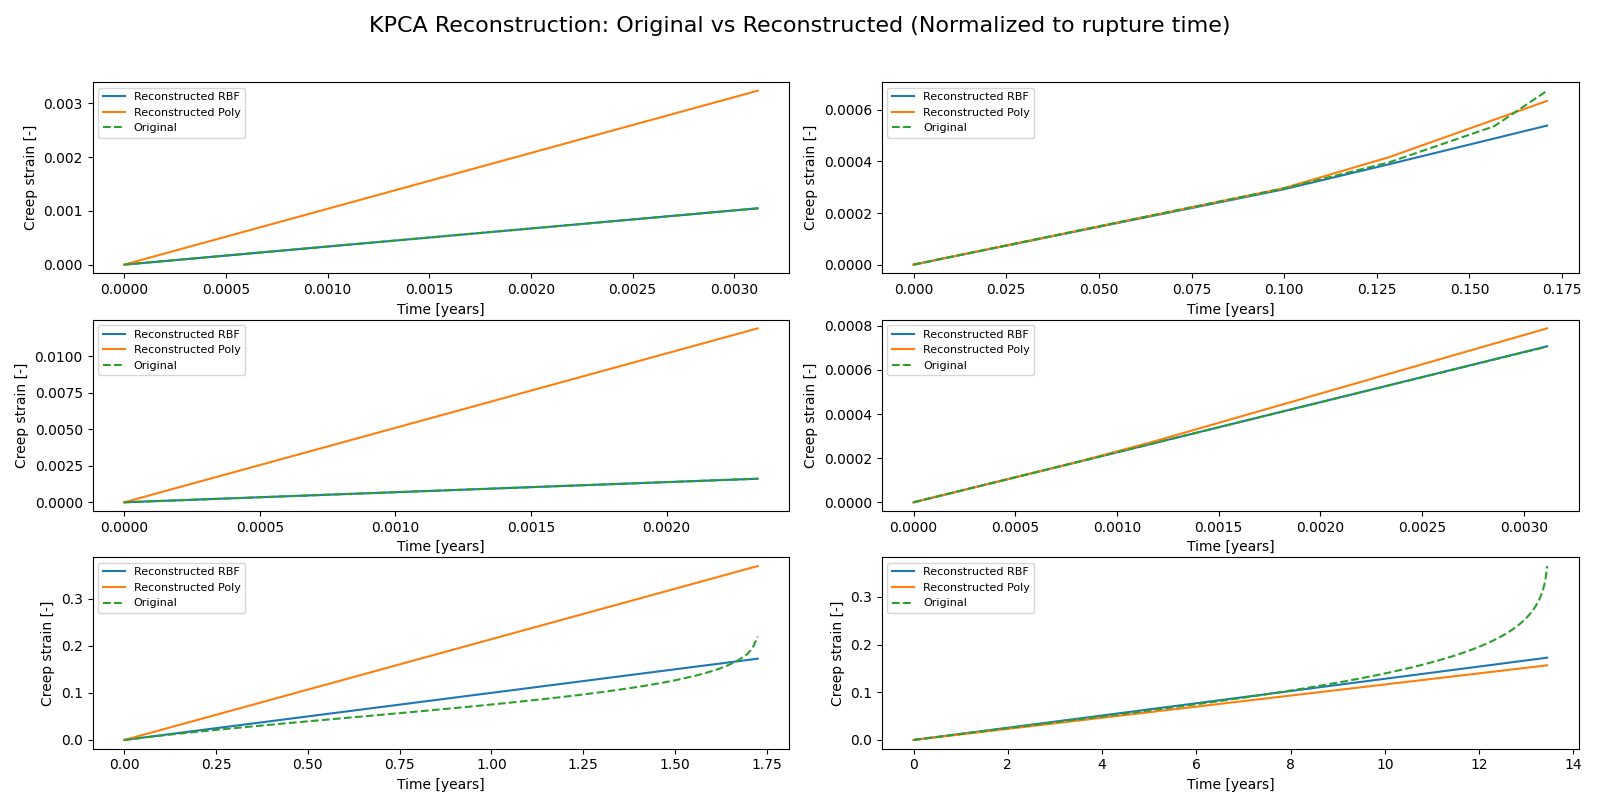
\includegraphics[width=1\textwidth]{figures/kpca_reconstructed_curves_norm.png}
		\caption{Original vs. Reconstructed Creep Curves(KPCA) - Normalization by rupture time approach.}
		\label{fig:kpca_norm_rupture_time}
	\end{figure}
	
	\subsection{Morch Model Parameter Representations (Inverse Model)}
	\label{Subsection::Results_Supervised}
	
	The parity plots for the seven Morch model parameters are shown in this section for each of the Regression models. The data points are coloured by the stress/load applied.
	
	\subsubsubsection{Random Forest Regression}
	
	Figure~\ref{fig:RF_regression} shows the parity plot for the Morch material model parameters as predicted by the Random Forest Regressor.
	
	\begin{figure}[H]
		\centering
		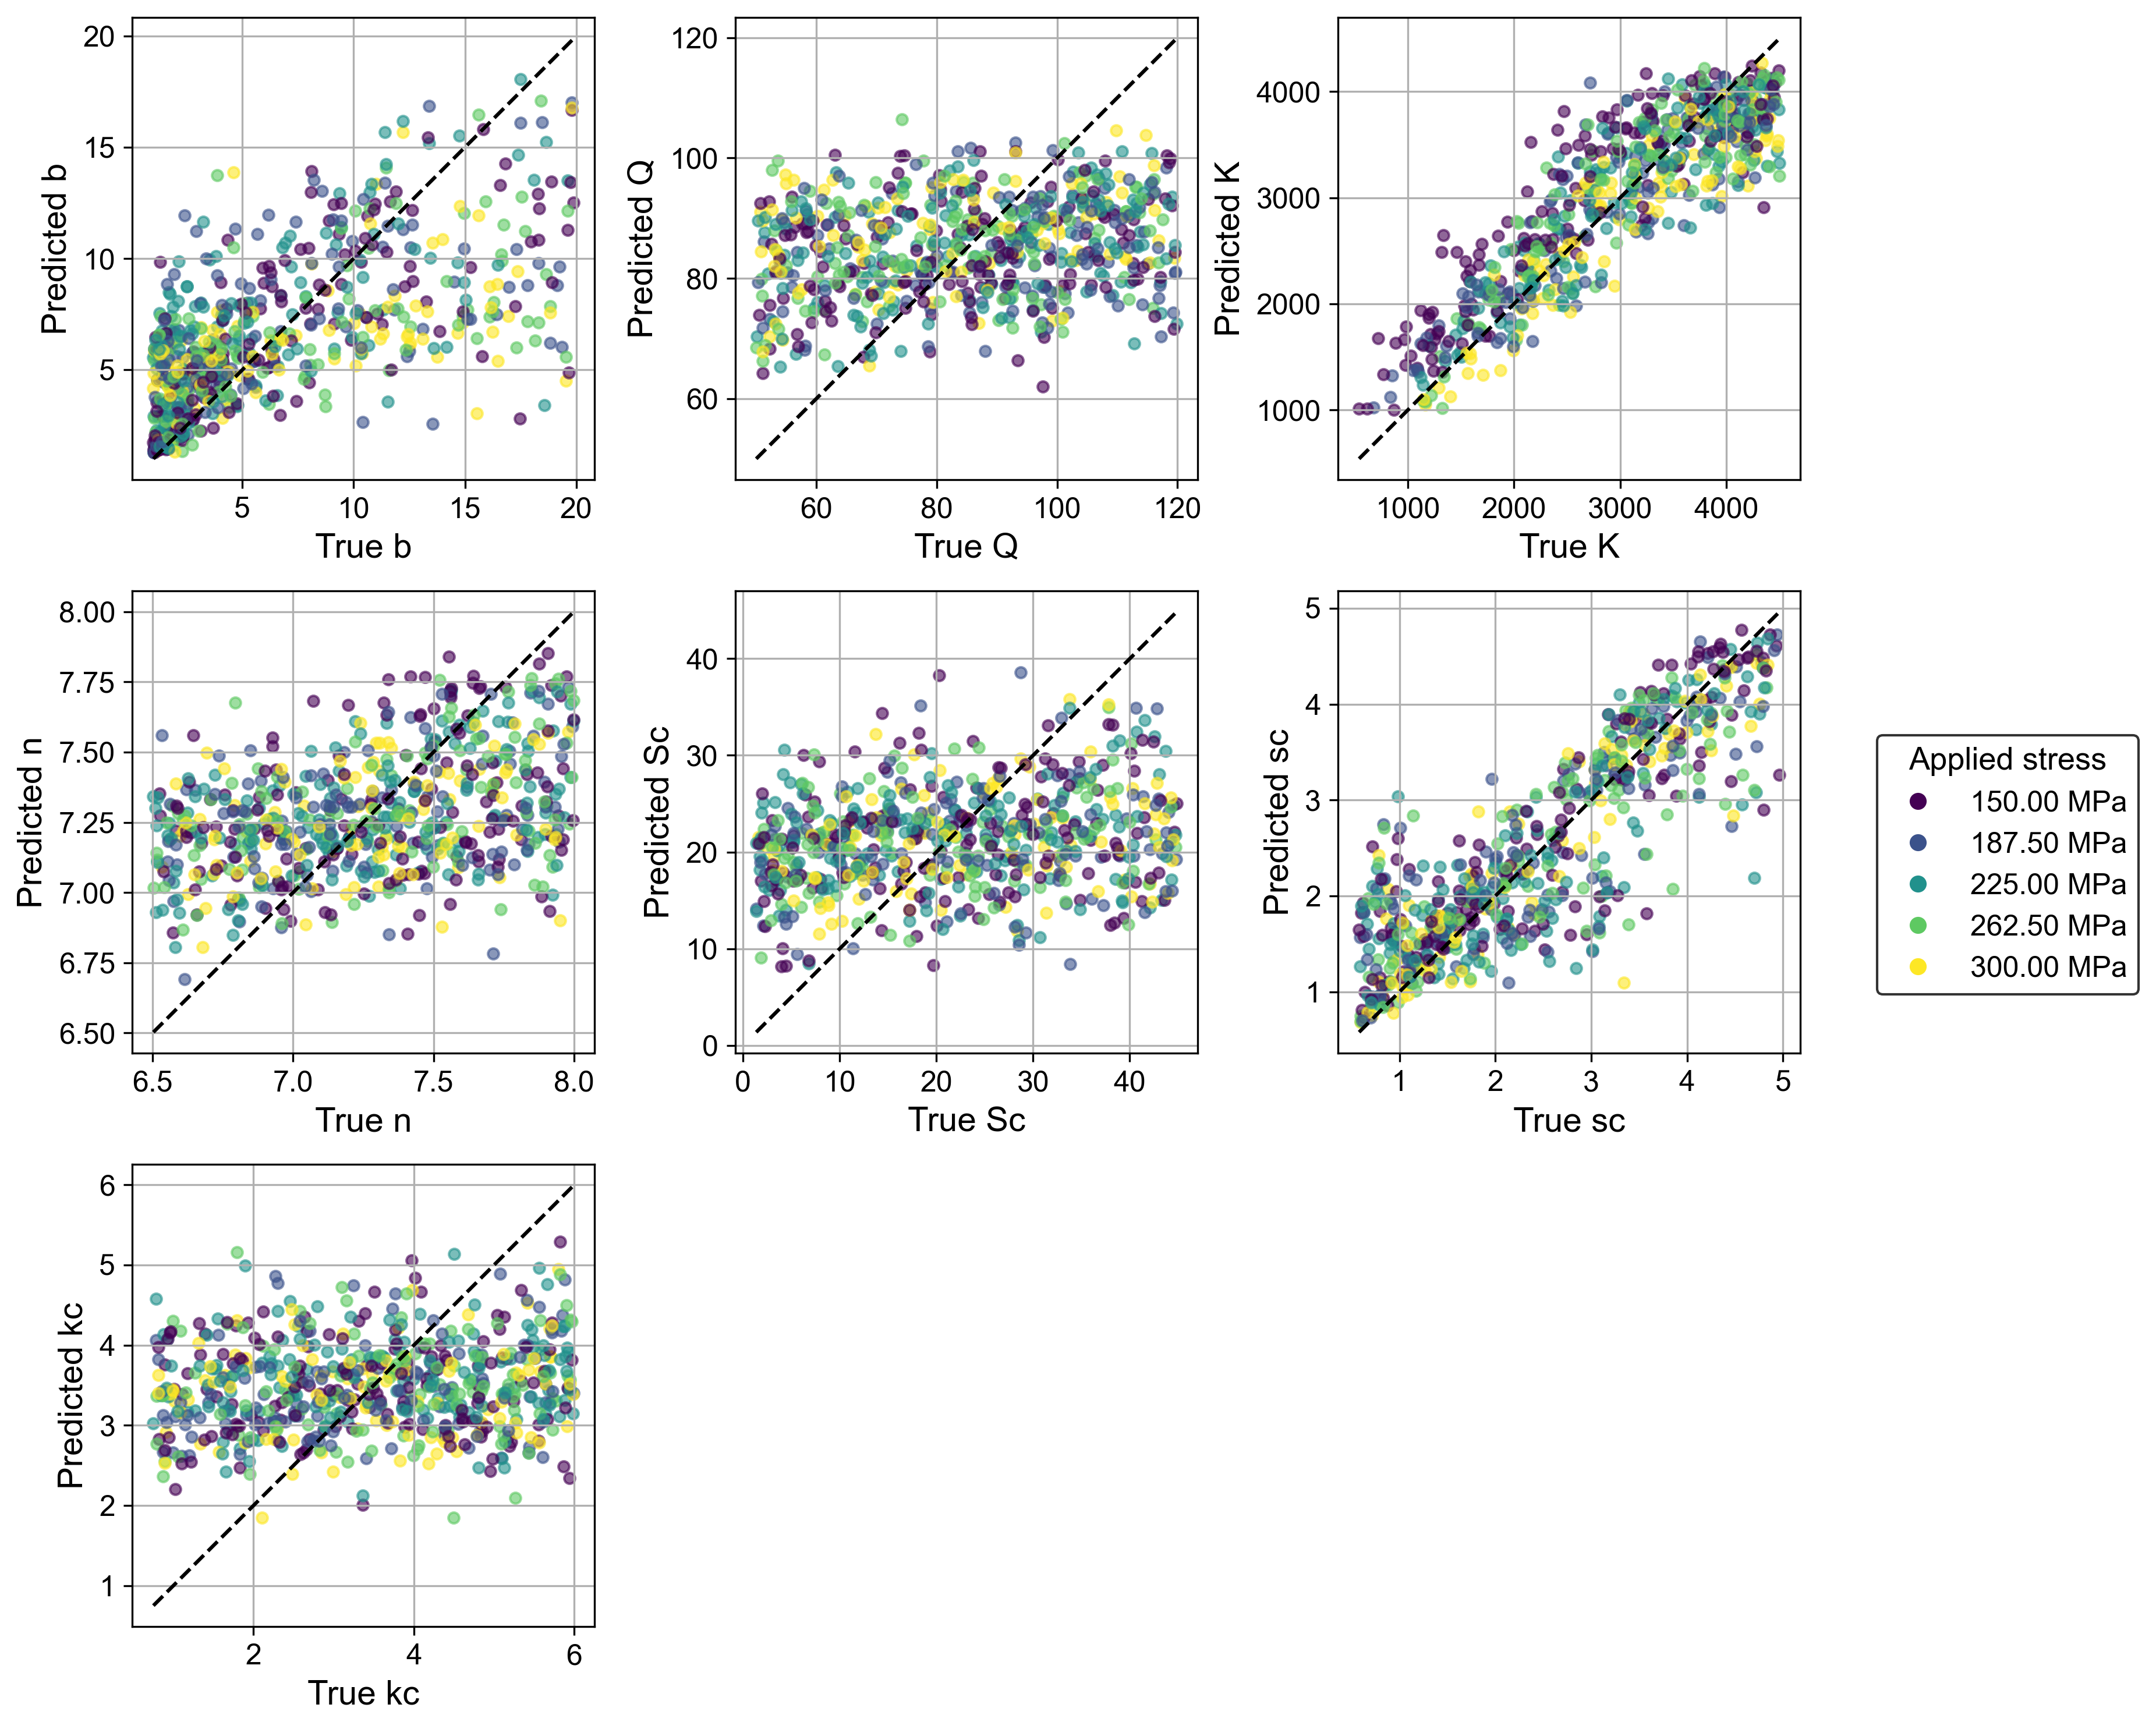
\includegraphics[width=0.95\textwidth]{figures/RF_parity_colored_by_load.png}
		\caption{Parity plot for the material model parameters predicted by random forest regressor.}
		\label{fig:RF_regression}
	\end{figure}
	
	\subsubsubsection{Gradient Boosting Regression}
	
	Figure~\ref{fig:GB_regression} shows the parity plot for the Morch material model parameters as predicted by the Gradient Boosting Regressor.
	
	\begin{figure}[H]
		\centering
		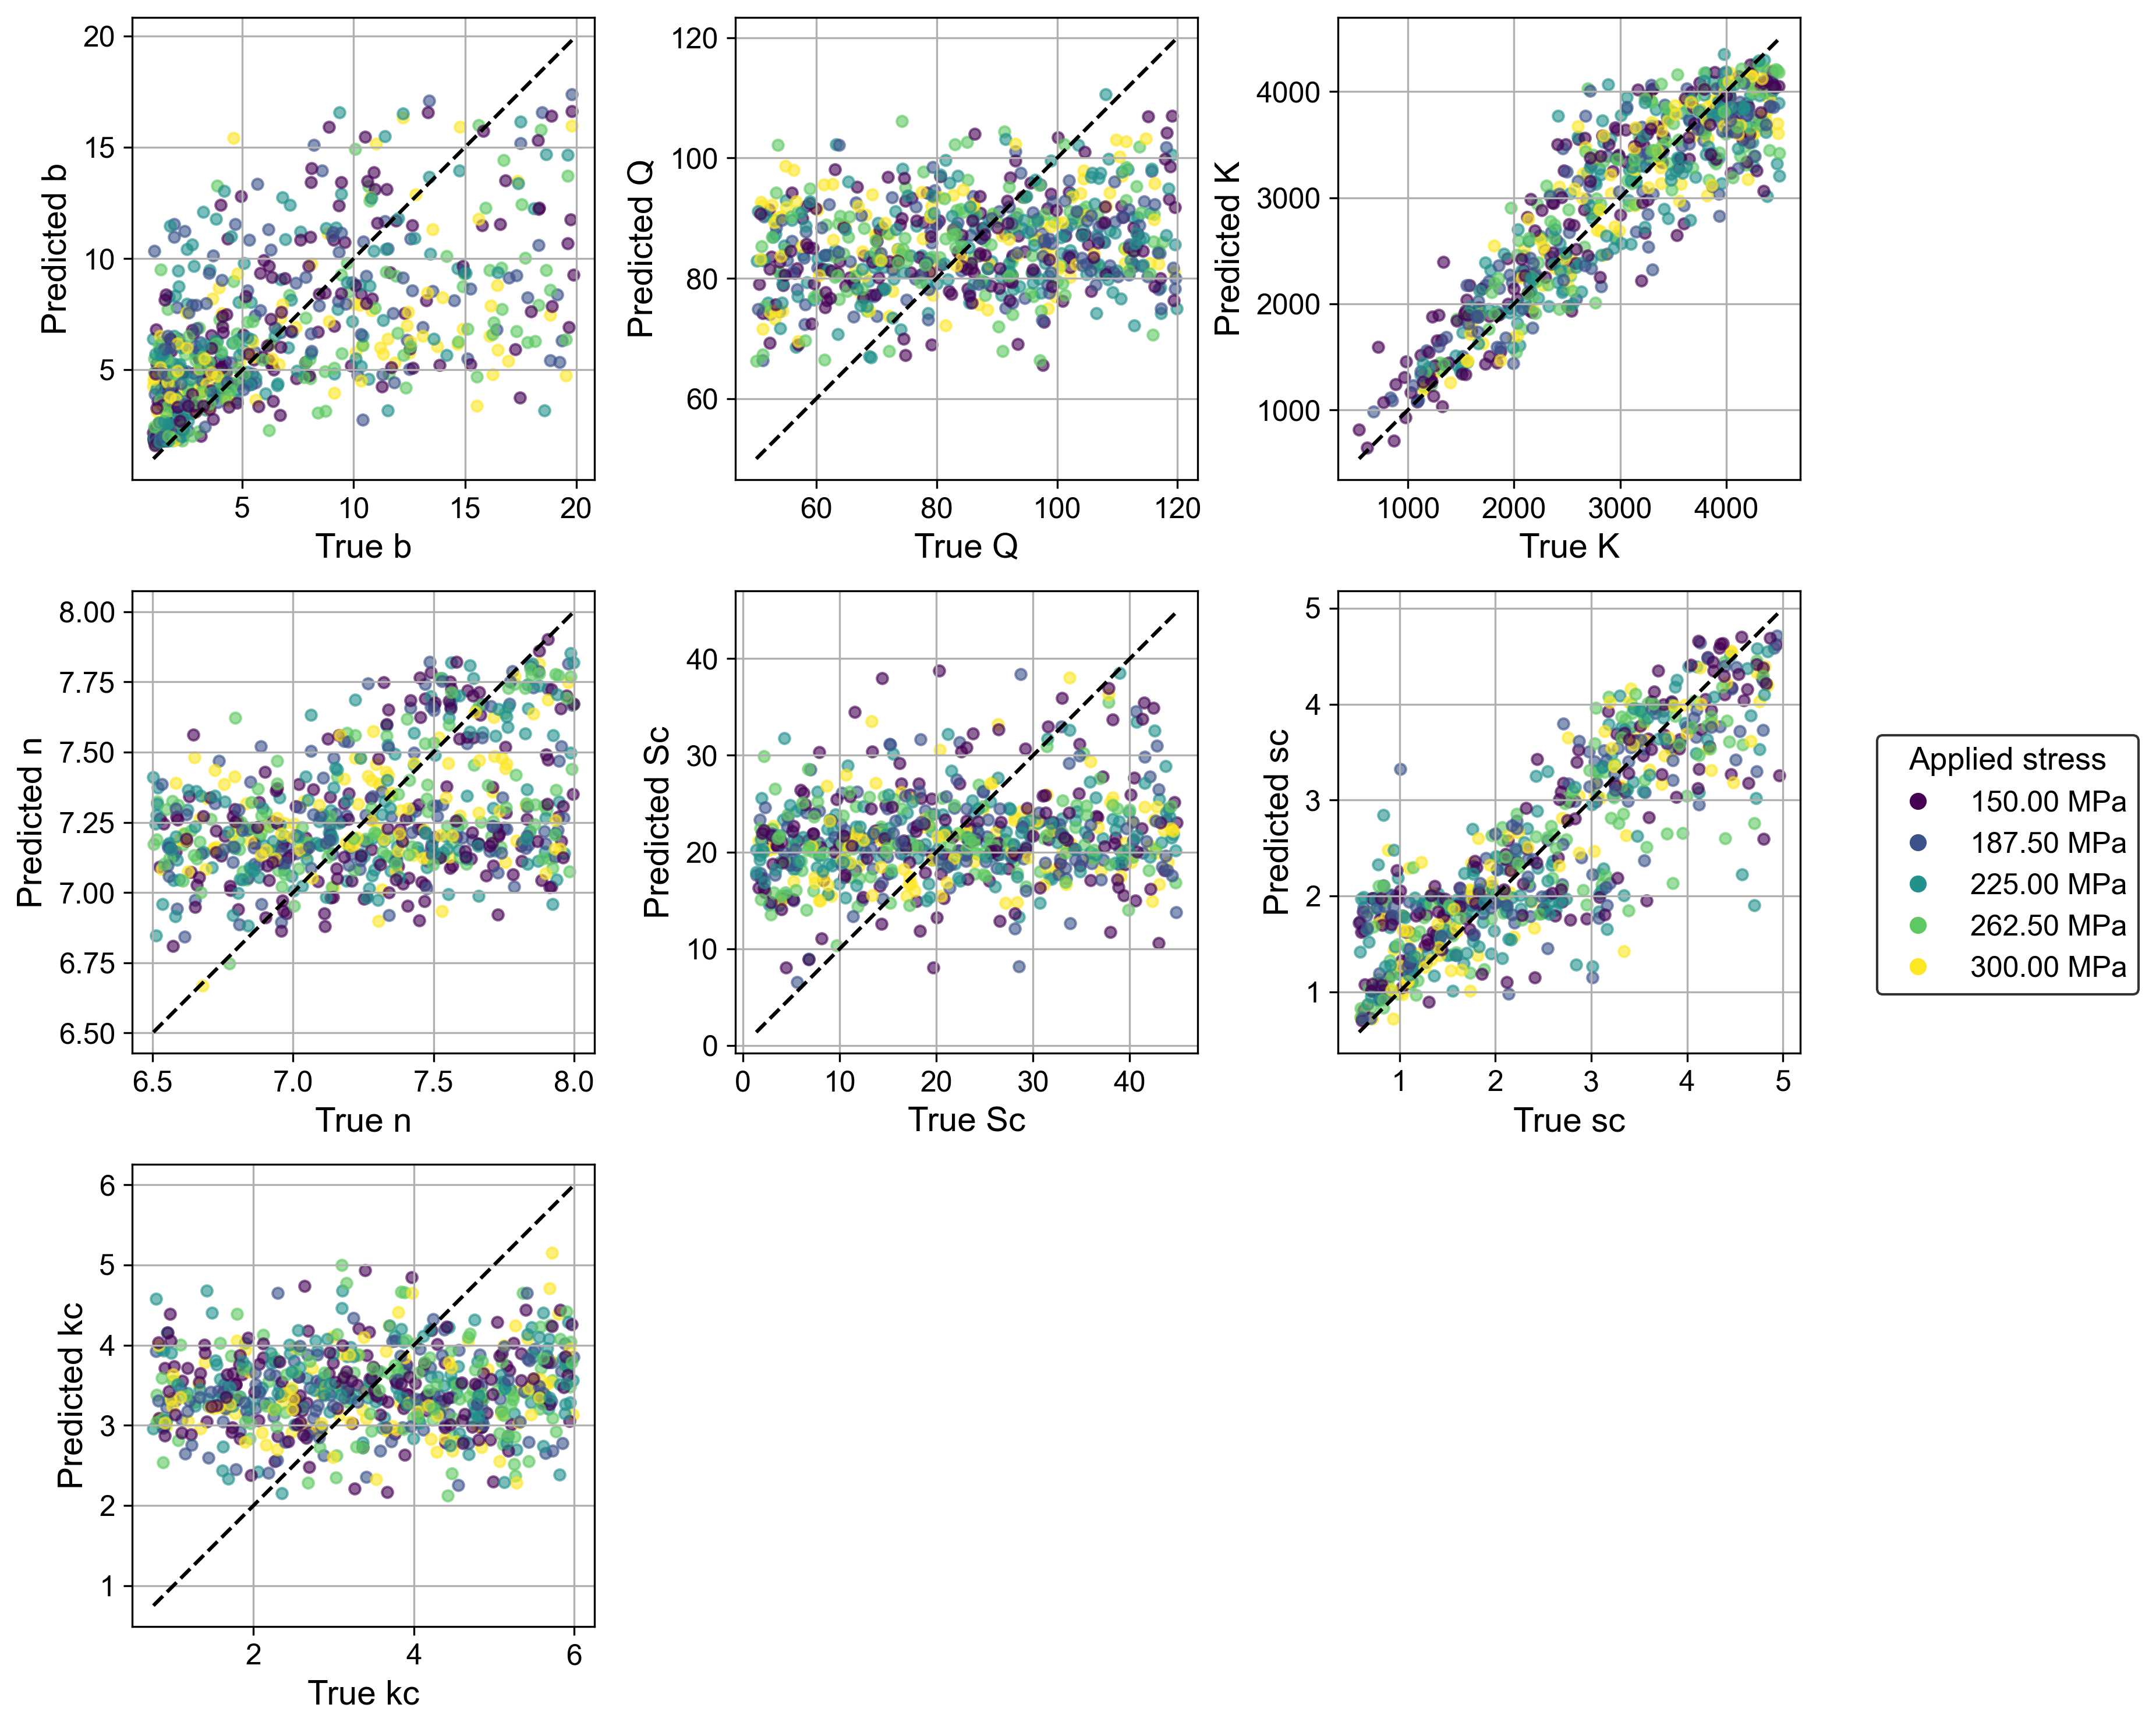
\includegraphics[width=0.95\textwidth]{figures/GB_parity_colored_by_load.png}
		\caption{Parity plot for the material model parameters predicted by gradient boosting regressor.}
		\label{fig:GB_regression}
	\end{figure}
	
	\subsubsubsection{Stacking Regression}
	
	Figure~\ref{fig:stacking_regression} shows the parity plot for the Morch material model parameters as predicted by the Stacking Regressor.
	
	\begin{figure}[H]
		\centering
		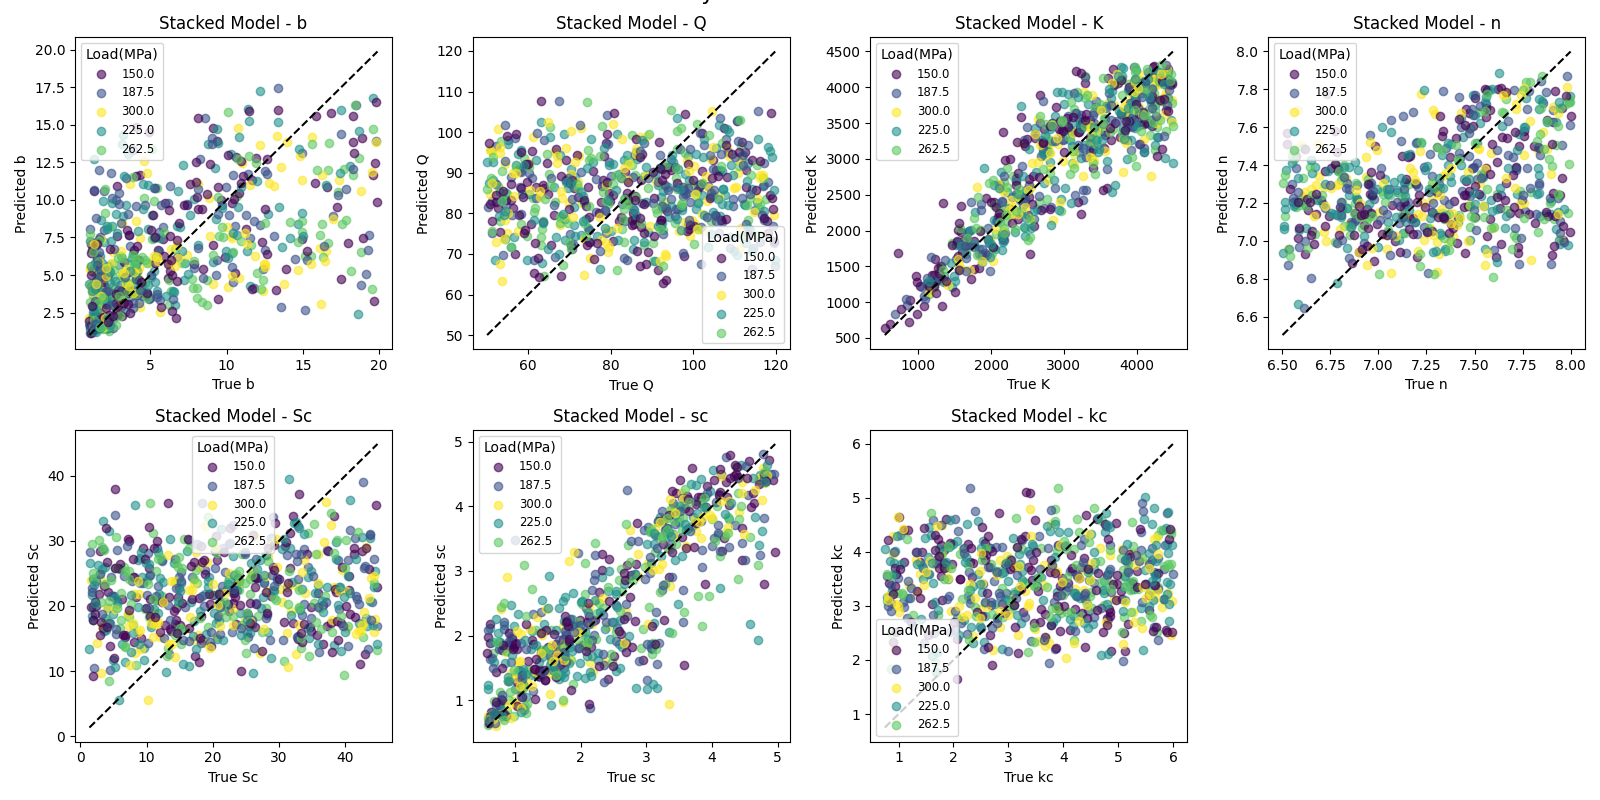
\includegraphics[width=0.95\textwidth]{figures/SM_parity_colored_by_load.png}
		\caption{Parity plot for the material model parameters predicted by stacking regressor.}
		\label{fig:stacking_regression}
	\end{figure}
	
	\subsubsubsection{Voting Regression}
	
	Figure~\ref{fig:voting_regression} shows the parity plot for the Morch material model parameters as predicted by the Voting Regressor.
	
	\begin{figure}[H]
		\centering
		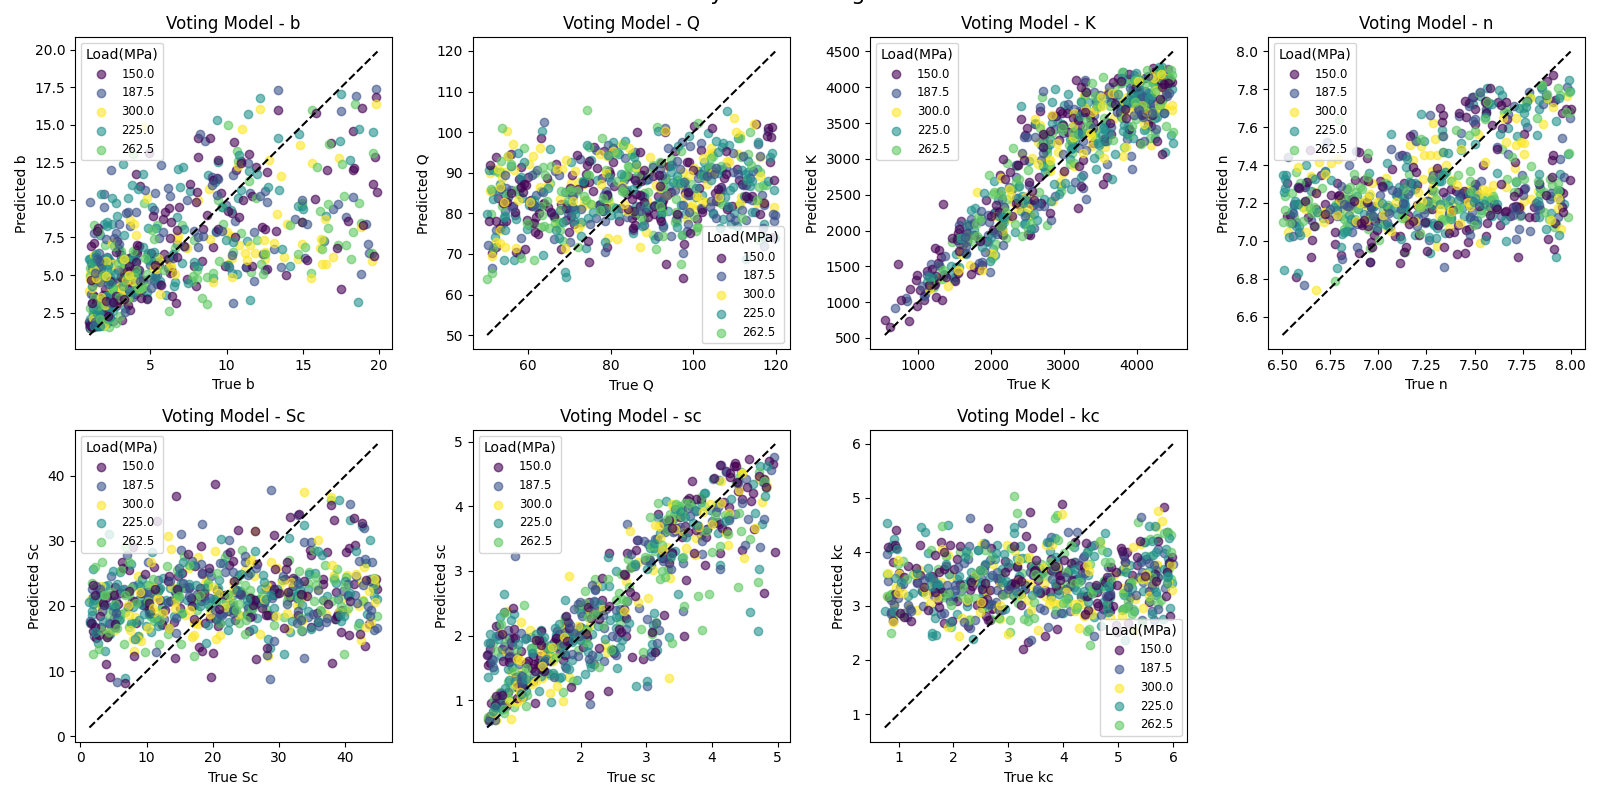
\includegraphics[width=0.95\textwidth]{figures/VM_parity_colored_by_load.png}
		\caption{Parity plot for the material model parameters predicted by voting regressor.}
		\label{fig:voting_regression}
	\end{figure}
	 
	Each model was evaluated on the 20\% test set using the metrics described in Section~\ref{Section::Evaluation}. Table~\ref{tab:model_performance} summarizes the mean absolute error (MAE) and $R^2$-score for predicting material model parameters.
	
	\begin{table}[ht]
		\centering
		\caption{Model performance comparison using MAE and $R^2$ score}
		\begin{tabular}{|l|c|c|}
			\hline
			\textbf{Model} & \textbf{Mean Absolute Error (MAE)} & \boldmath$R^2$ \\
			\hline
			Random Forest    & 58.3825 & 0.2890 \\
			Gradient Boosting & 53.9970 & 0.2830 \\
			Stacking Model   & 56.7212 & 0.1904 \\
			Voting Model     & 52.4986 & 0.2996 \\
			\hline
		\end{tabular}
		\label{tab:model_performance}
	\end{table}
	
	Since the Voting model shows better results among the four, it is used to generate creep curves from the finite element solver using the predicted material parameters. The figure~\ref{fig:curve_recon_model_params} shows the comparison of the original vs. the reconstructed creep curves.	
		
	\begin{figure}[H]
		\centering
		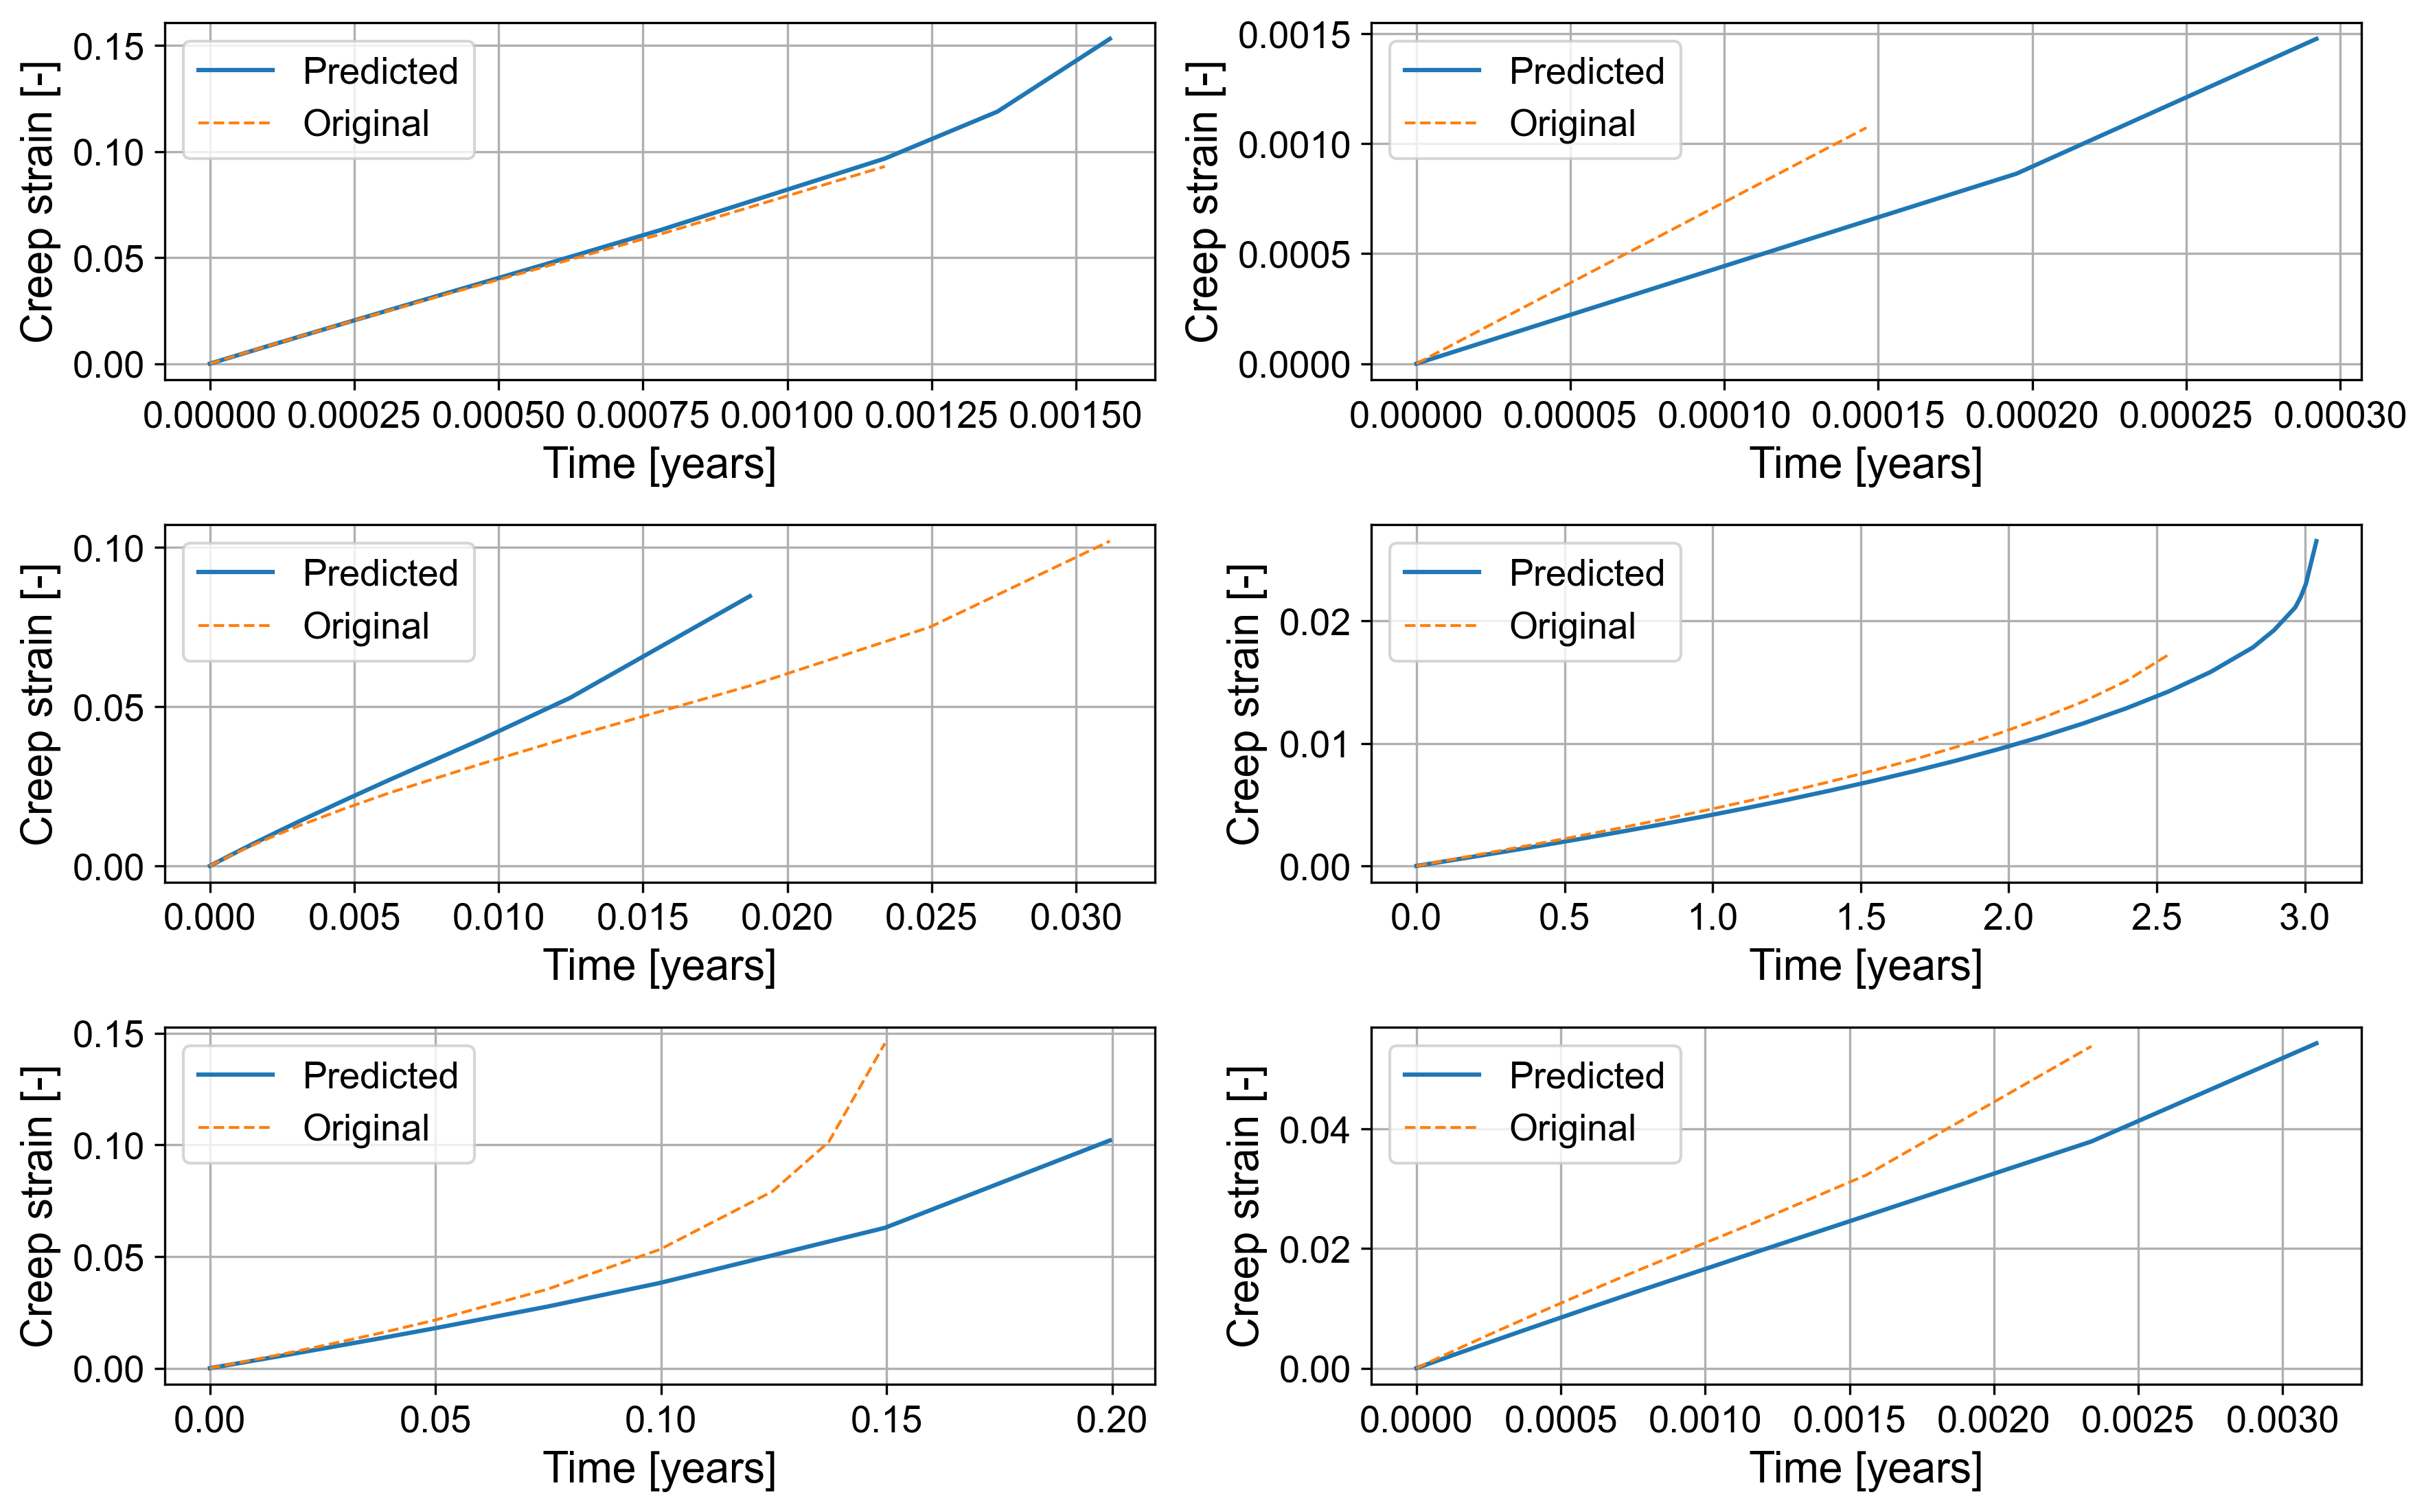
\includegraphics[width=1\textwidth]{figures/creep_comparison_from_model_params.png}
		\caption{Comparison of predicted and actual creep curves using Voting Regressor on test data.}
		\label{fig:curve_recon_model_params}
	\end{figure}
	
	\subsection{Model Comparison}
	\label{Subsection::Results_ModelComparison}
	
	The models discussed in section~\ref{Section::Results_CreepCurveRepresentations} are compared based on metrics like RMSE, minimum creep rate error and time to rupture prediction error.
	
	Figure~\ref{fig:rmse_reconstruction_errors} shows the histogram of RMSE for the different models.
	\begin{figure}[H]
		\centering
		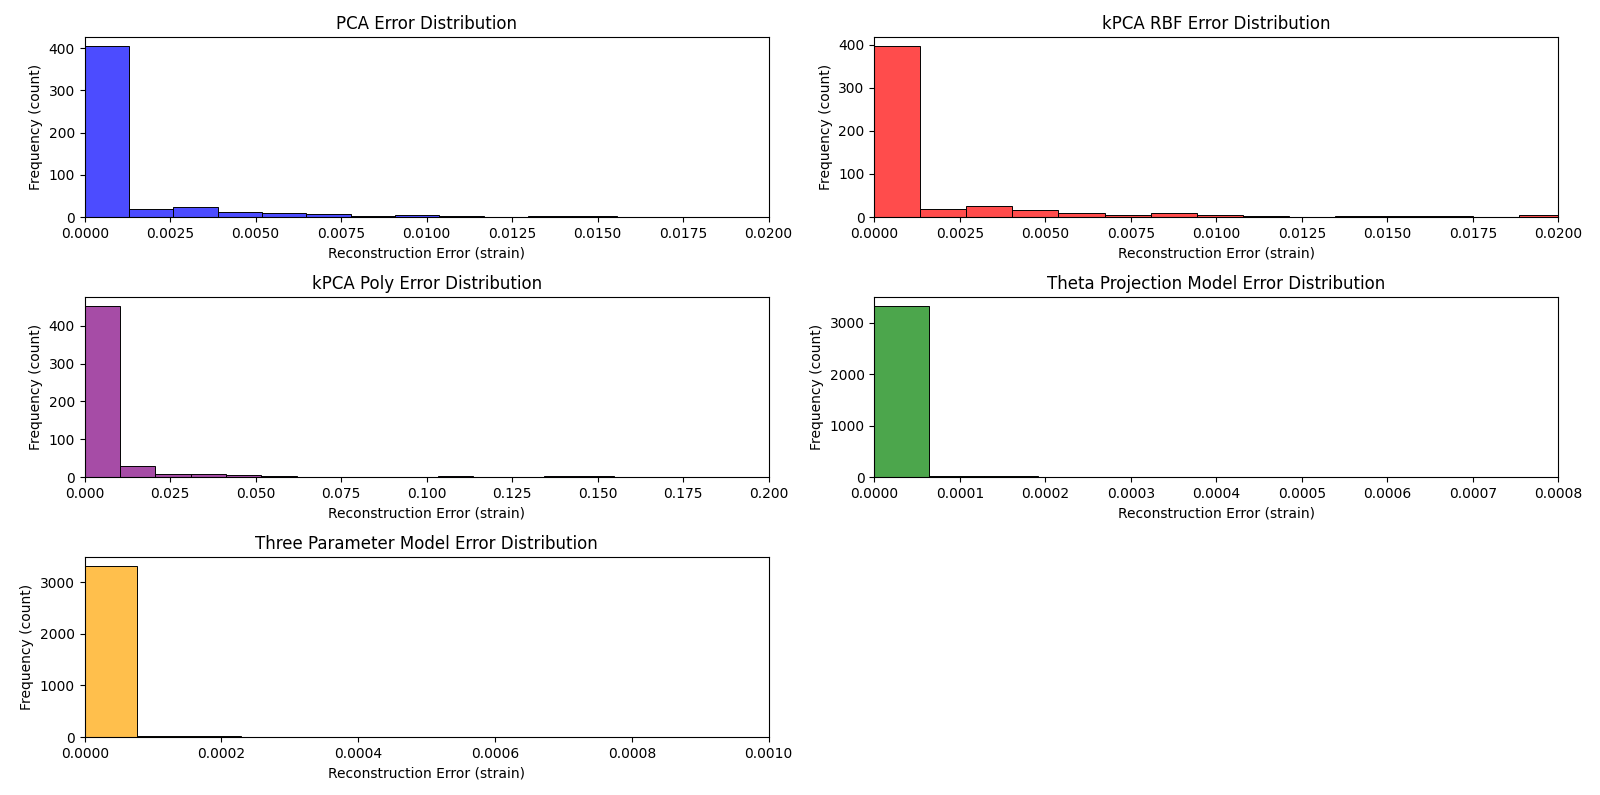
\includegraphics[width=1\textwidth]{figures/rmse_reconstruction_errors.png}
		\caption{RMSE histograms of different models.}
		\label{fig:rmse_reconstruction_errors}
	\end{figure}
	
	Figure~\ref{fig:min_creep_rate_error_hist} shows the histogram of minimum creep rate errors for the different models.
	\begin{figure}[H]
		\centering
		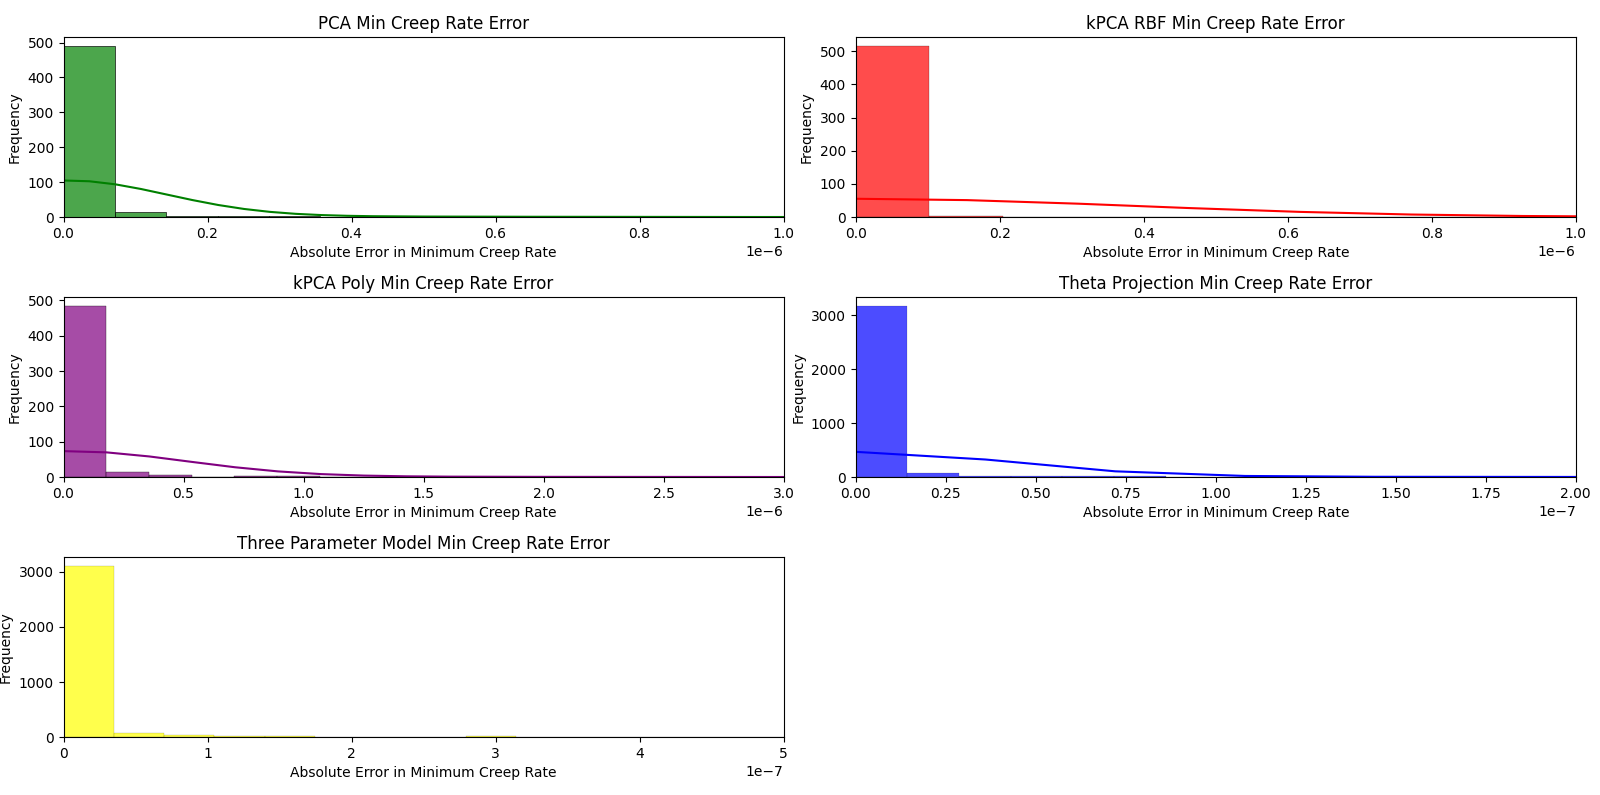
\includegraphics[width=1\textwidth]{figures/min_creep_rate_error_hist.png}
		\caption{Min. creep rate error histograms of different models.}
		\label{fig:min_creep_rate_error_hist}
	\end{figure}
	
	Figure~\ref{fig:fracture_time_error_hist} shows the histogram of time to rupture prediction for the different models.
	\begin{figure}[H]
		\centering
		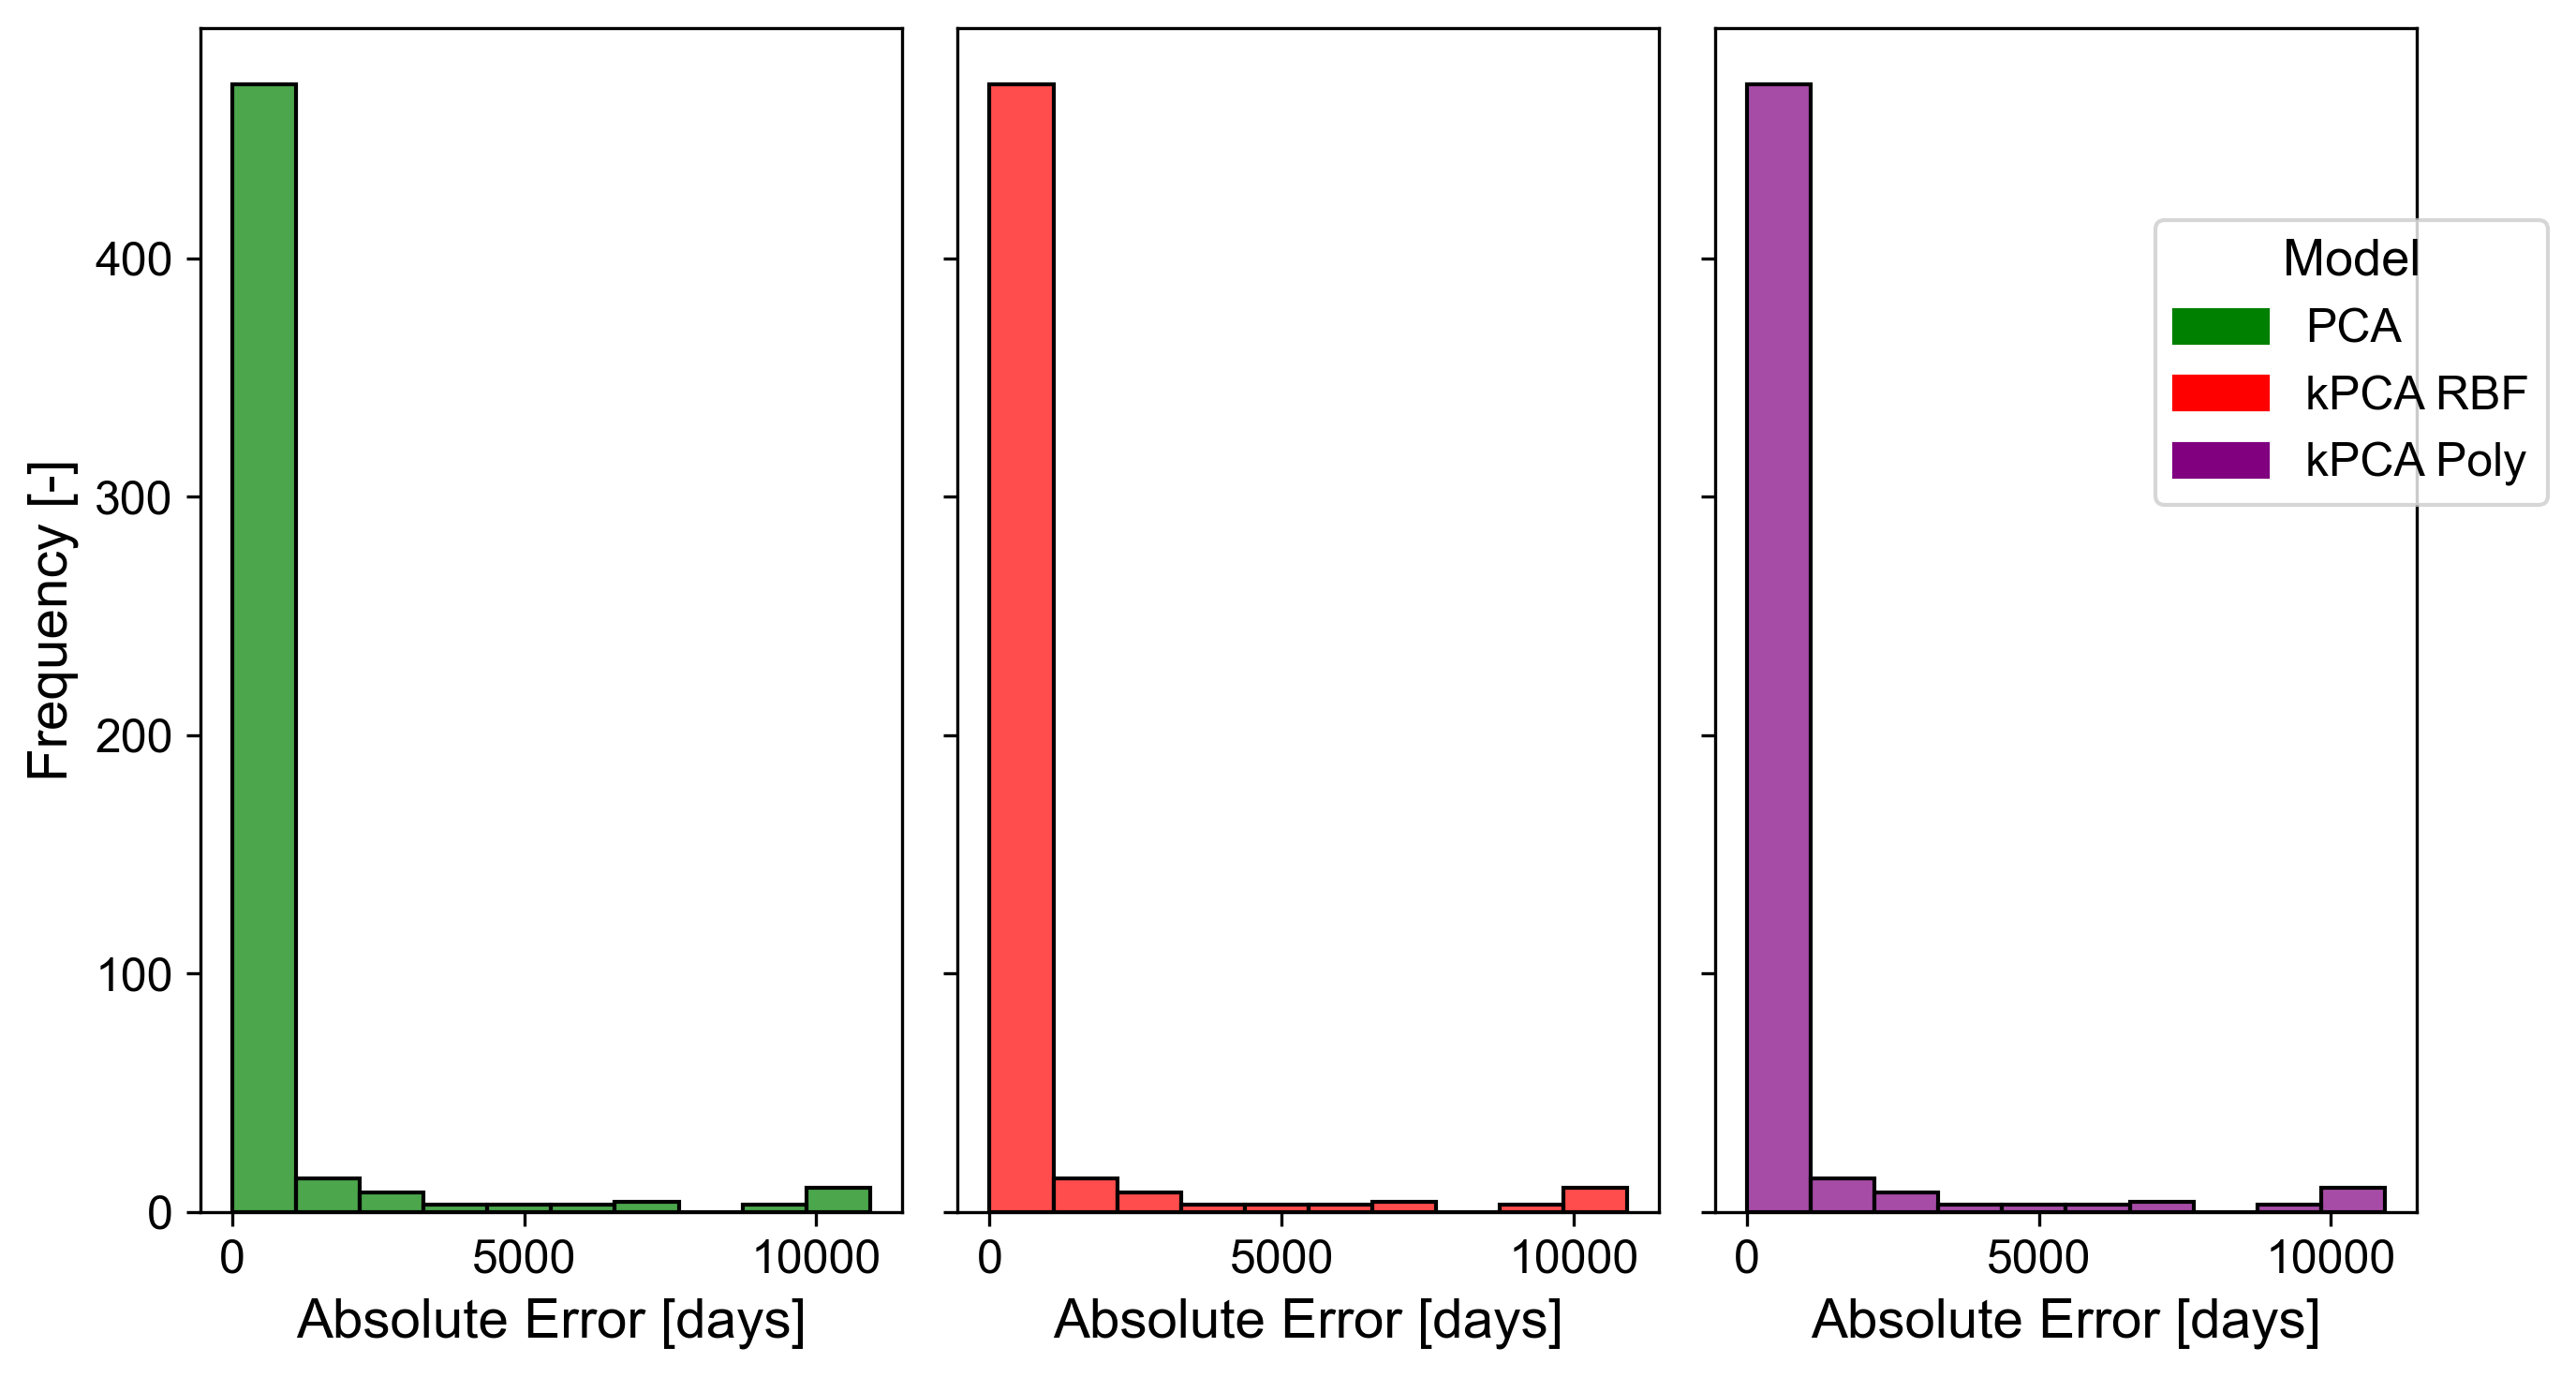
\includegraphics[width=0.9\textwidth]{figures/fracture_time_error_hist.png}
		\caption{Time to rupture prediction error histograms of different models.}
		\label{fig:fracture_time_error_hist}
	\end{figure}
	
	Table~\ref{tab:model_errors} shows the comparison between the different models already discussed in the section~\ref{Section::Results_CreepCurveRepresentations}.
	
	\begin{table}[ht]
		\centering
		\caption{Model Errors for the different Creep curve representations}
		\begin{tabularx}{\textwidth}{|X|X|X|X|X|X|}
			\hline
			\textbf{Metric} & \textbf{PCA} & \textbf{kPCA RBF} & \textbf{kPCA Poly} & \textbf{Theta Projection Model} & \textbf{Three Parameter Model} \\
			\hline
			\textbf{RMSE (Strain [-])} & 0.002683 & 0.002808 & 0.009904 & 0.000004 & 0.000007 \\
			\hline
			\textbf{Min. Creep Strain Rate} & $5.30 \times 10^{-8}$ & $6.22 \times 10^{-8}$ & $1.76 \times 10^{-7}$ & $1.54 \times 10^{-8}$ & $4.84 \times 10^{-8}$ \\
			\hline
			\textbf{Time to Rupture (days)} & 546 & 546 & 545 & - & - \\
			\hline
		\end{tabularx}
		\label{tab:model_errors}
	\end{table}
		
	\section{Active Learning Results}
	\label{Section::Results_AL}
	
	The active learning loop is run for 2000 iterations, selecting one new samples per iteration.	
	
	The Isolation Forest  classifier shows the convergence area of the material model parameters after the execution of the active learning loop. Figure~\ref{fig:pairwise_projections} shows the convergence of the pairwise projections mapping of the material model parameters.
	\begin{figure}[htbp]
		\centering
		\begin{tabular}{cccc}  % 4 columns
			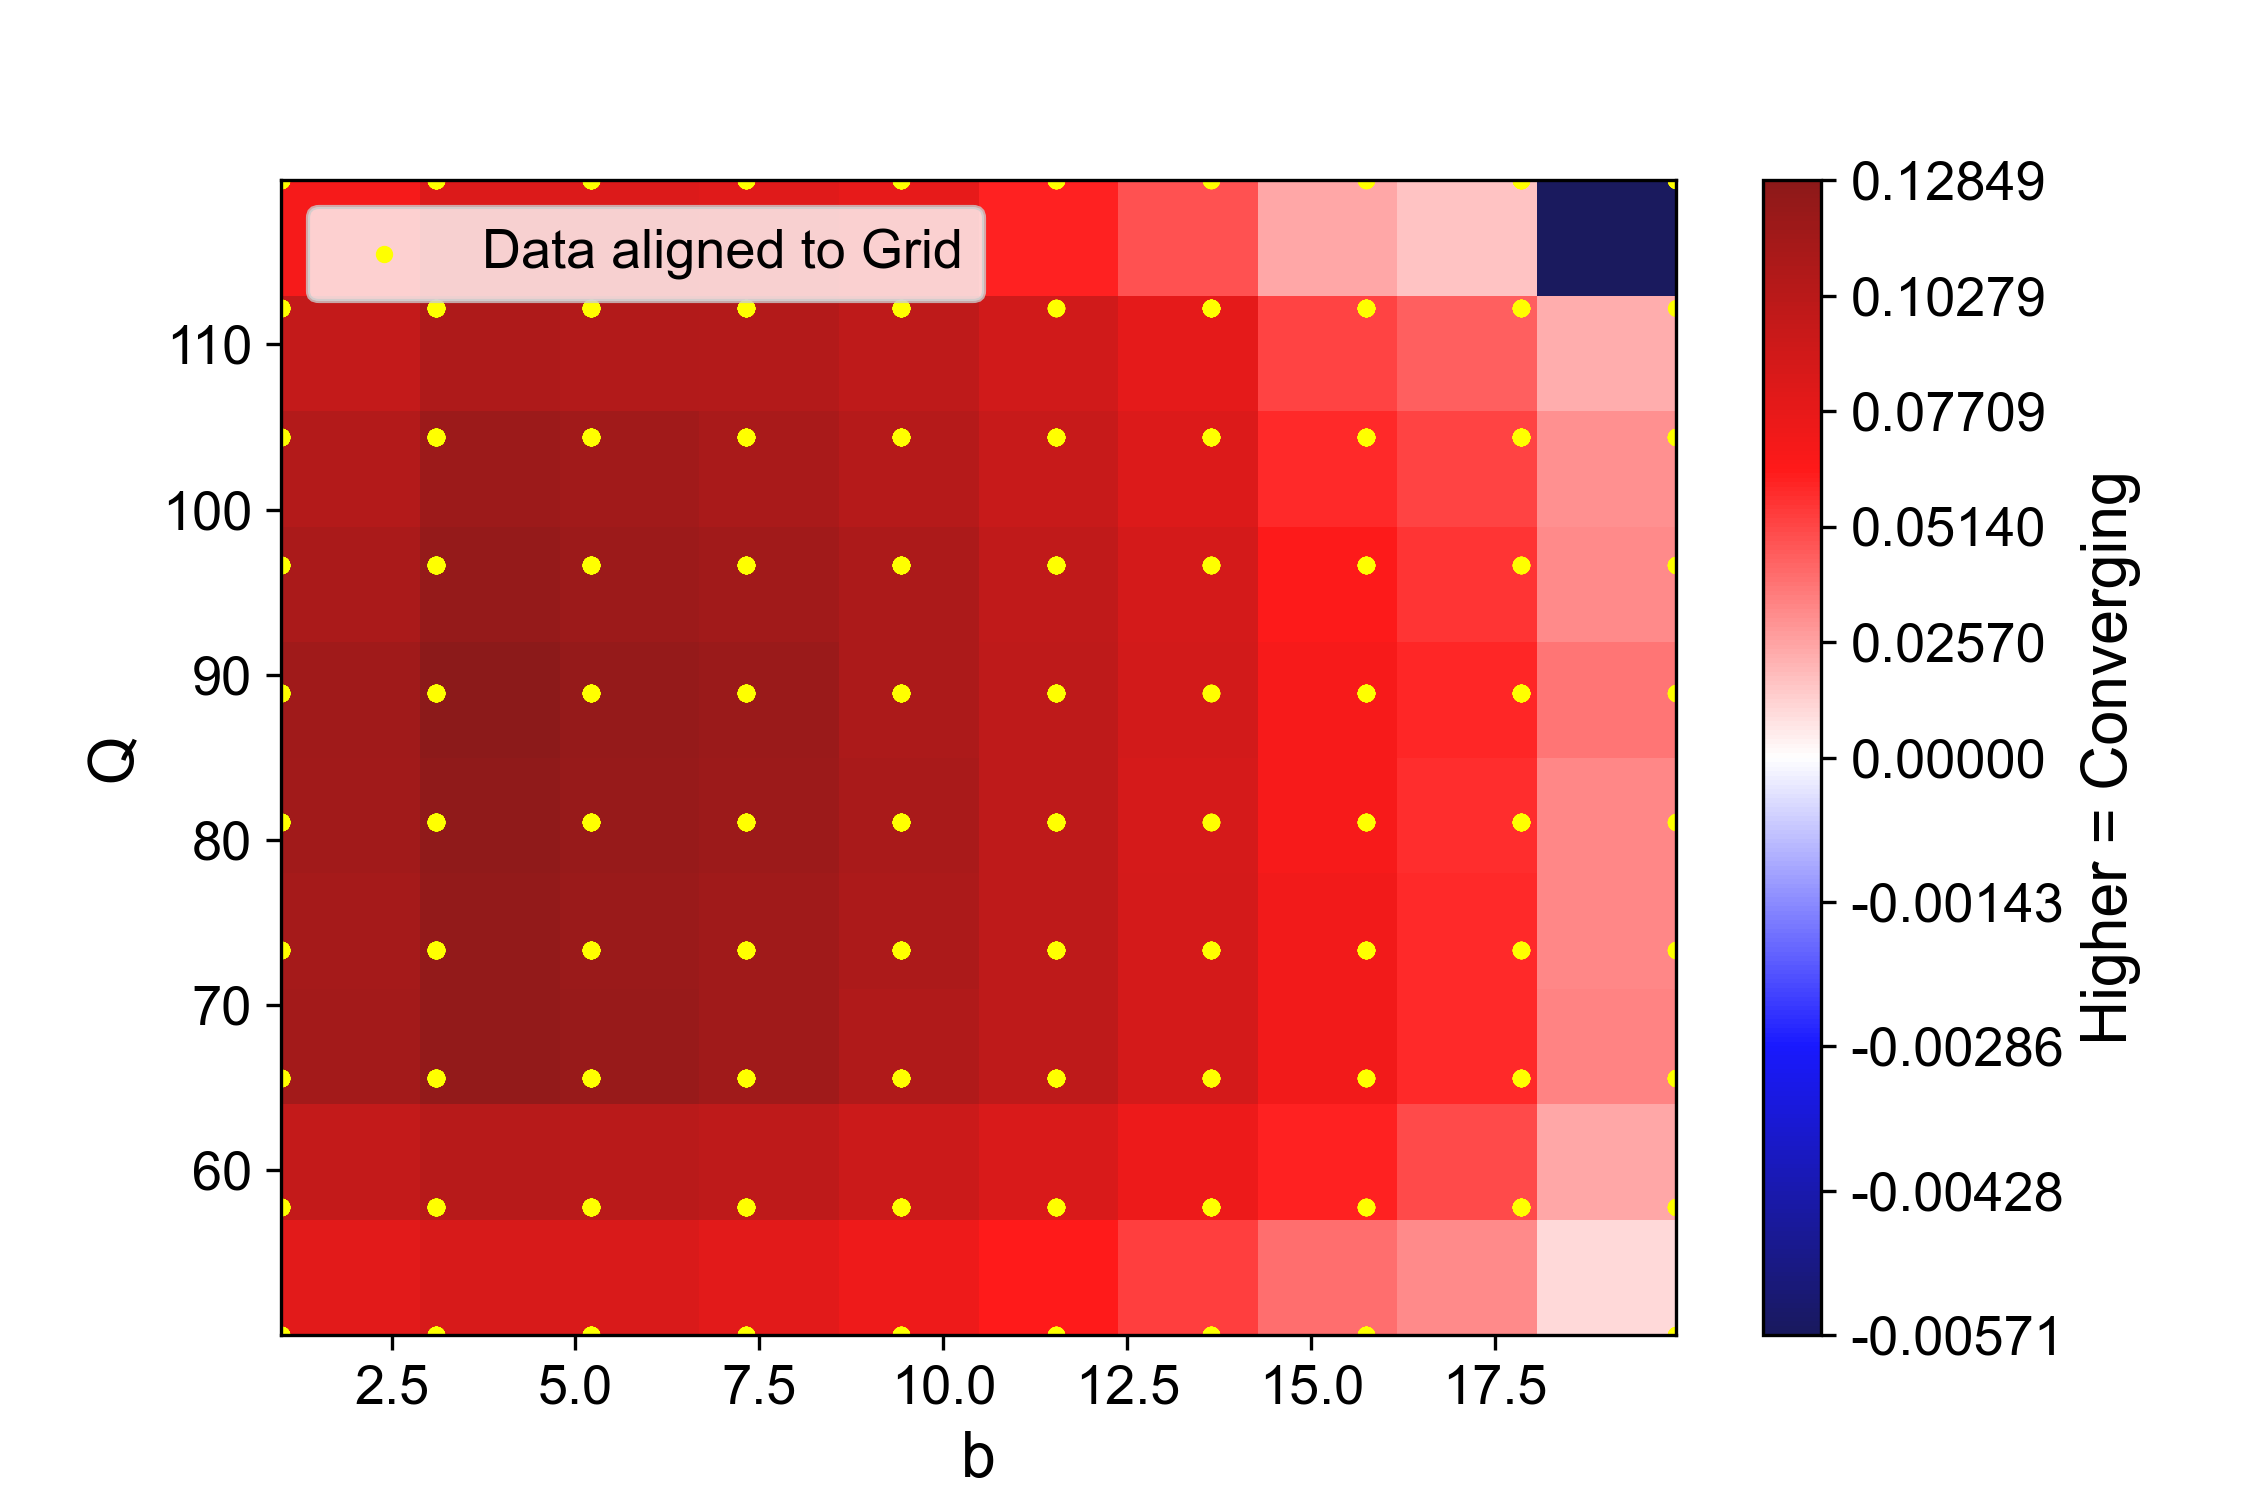
\includegraphics[width=0.32\textwidth]{figures/convergence/pairwise_projections_1.png} &
			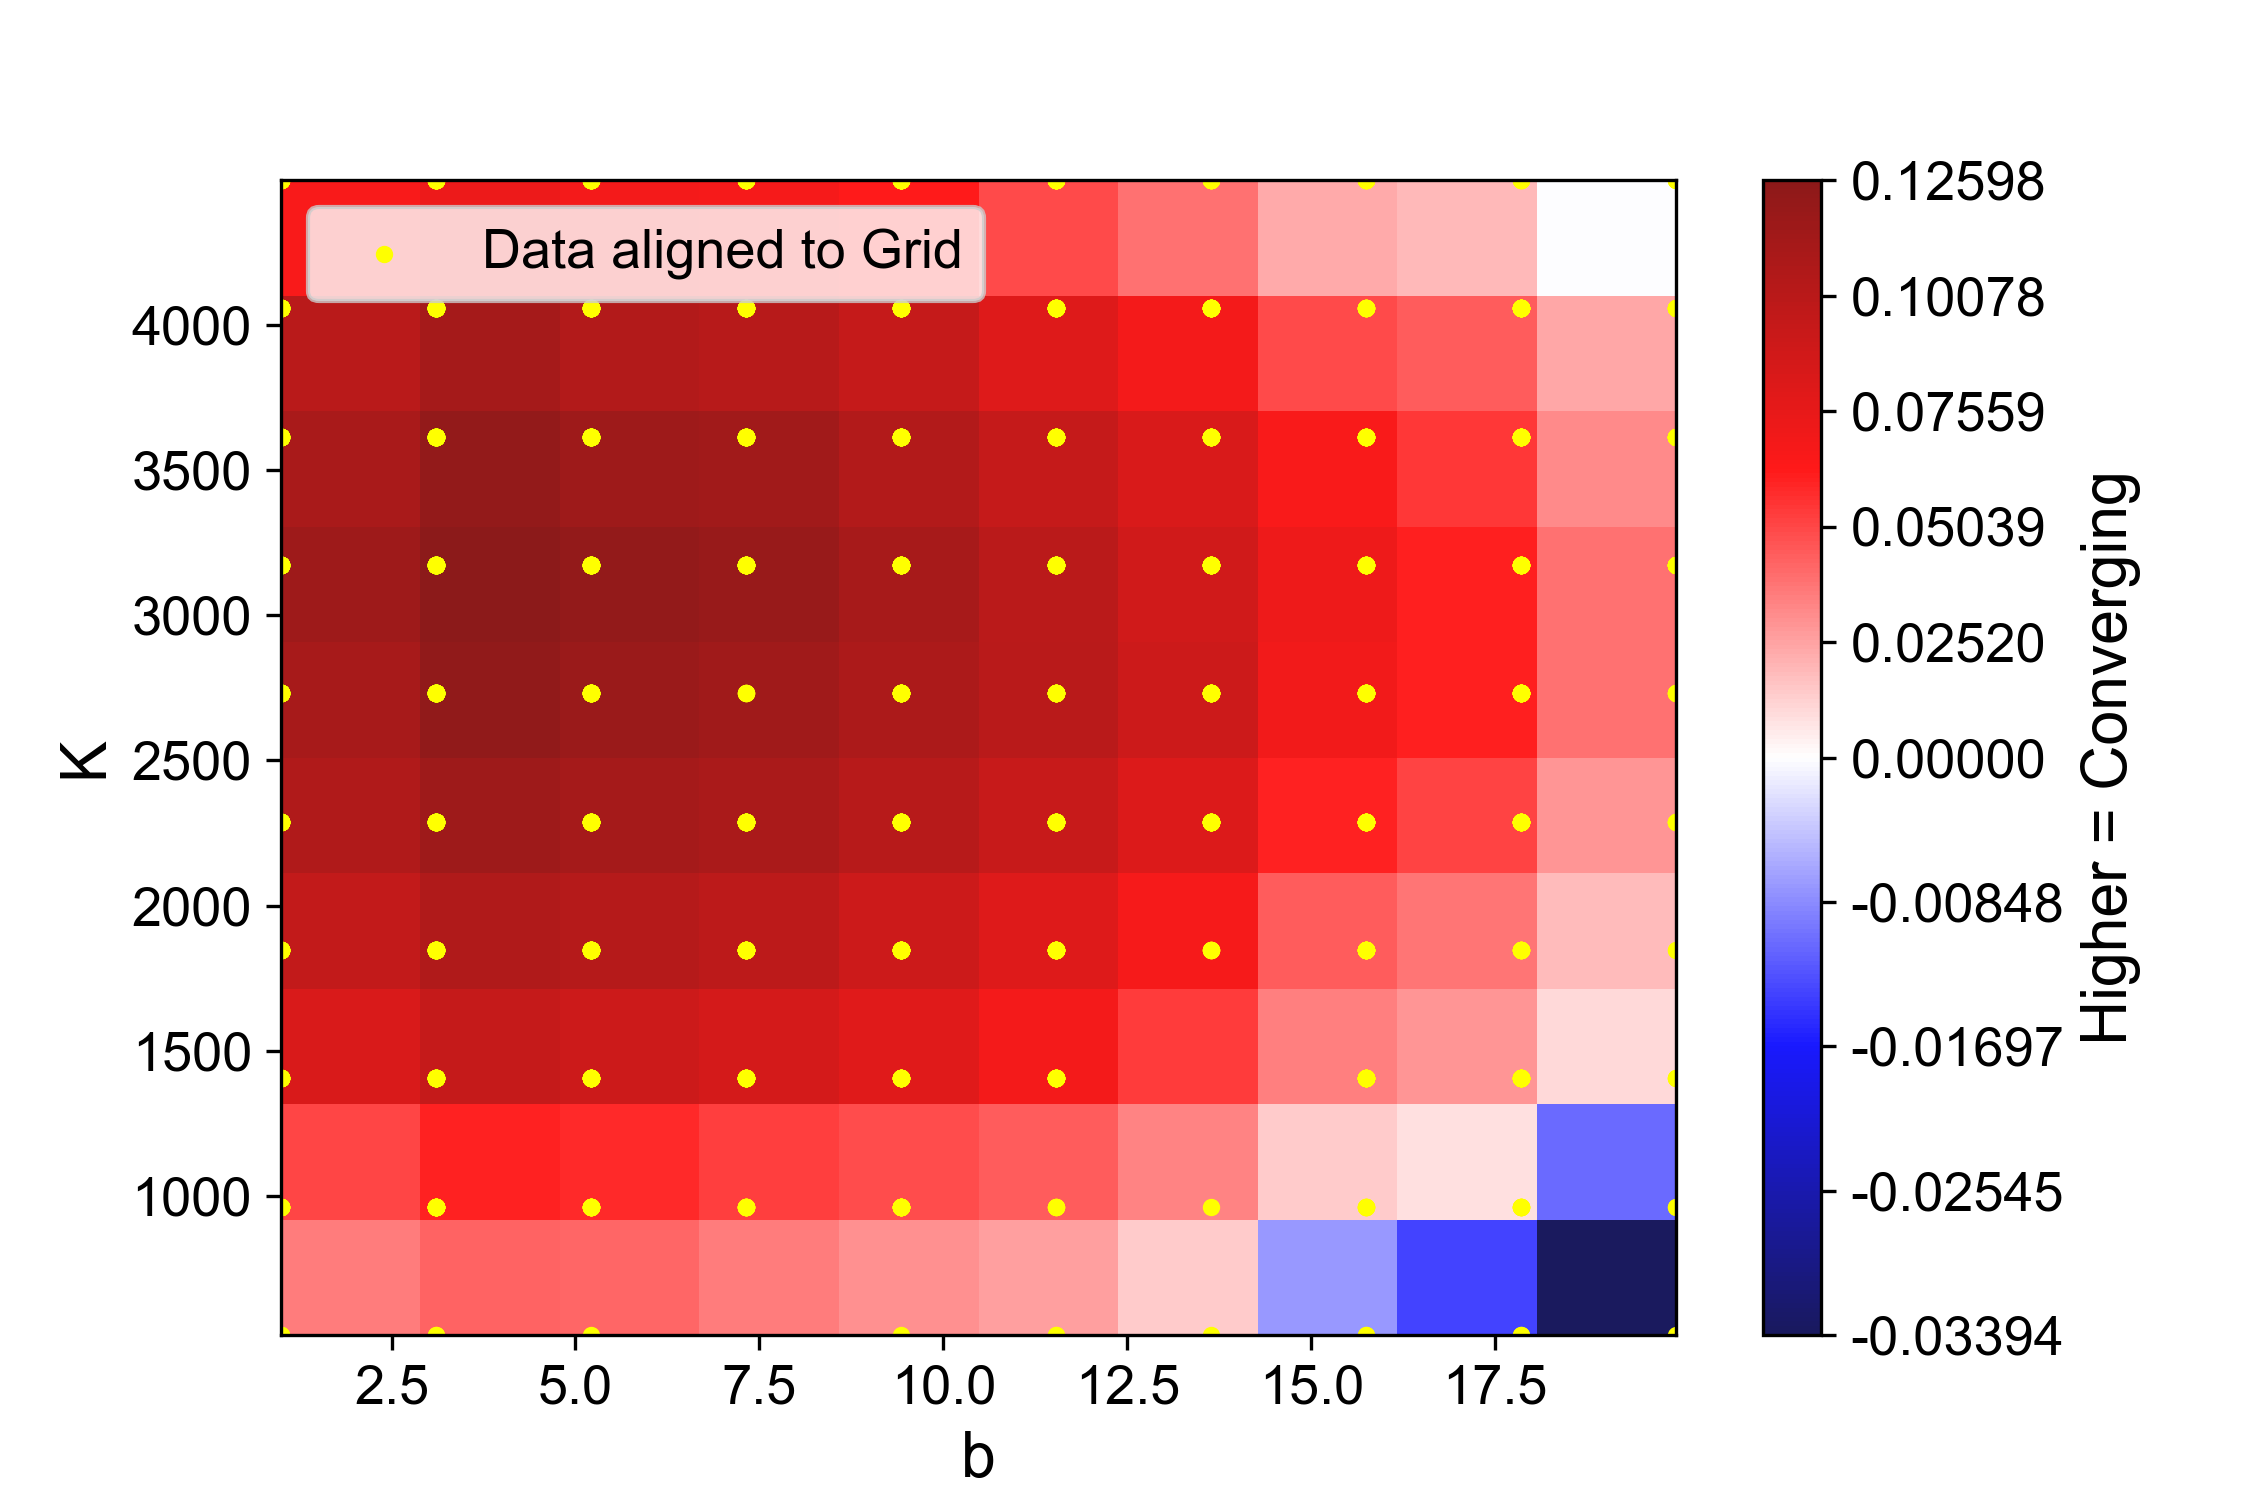
\includegraphics[width=0.32\textwidth]{figures/convergence/pairwise_projections_2.png} &
			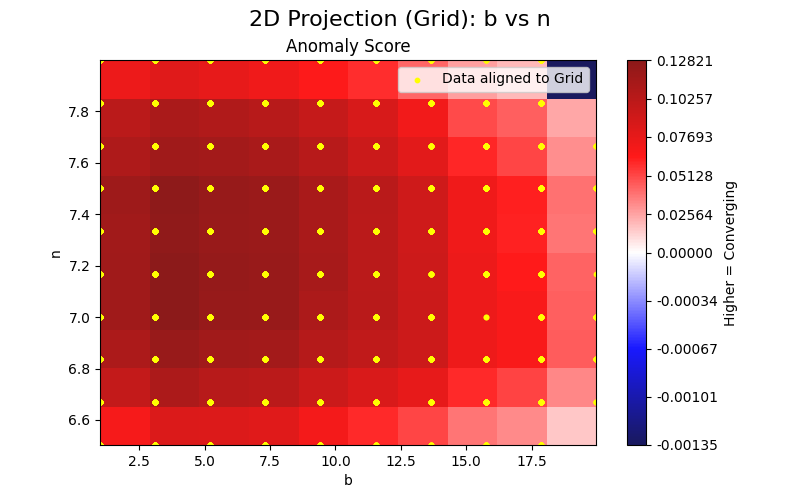
\includegraphics[width=0.32\textwidth]{figures/convergence/pairwise_projections_3.png} \\
			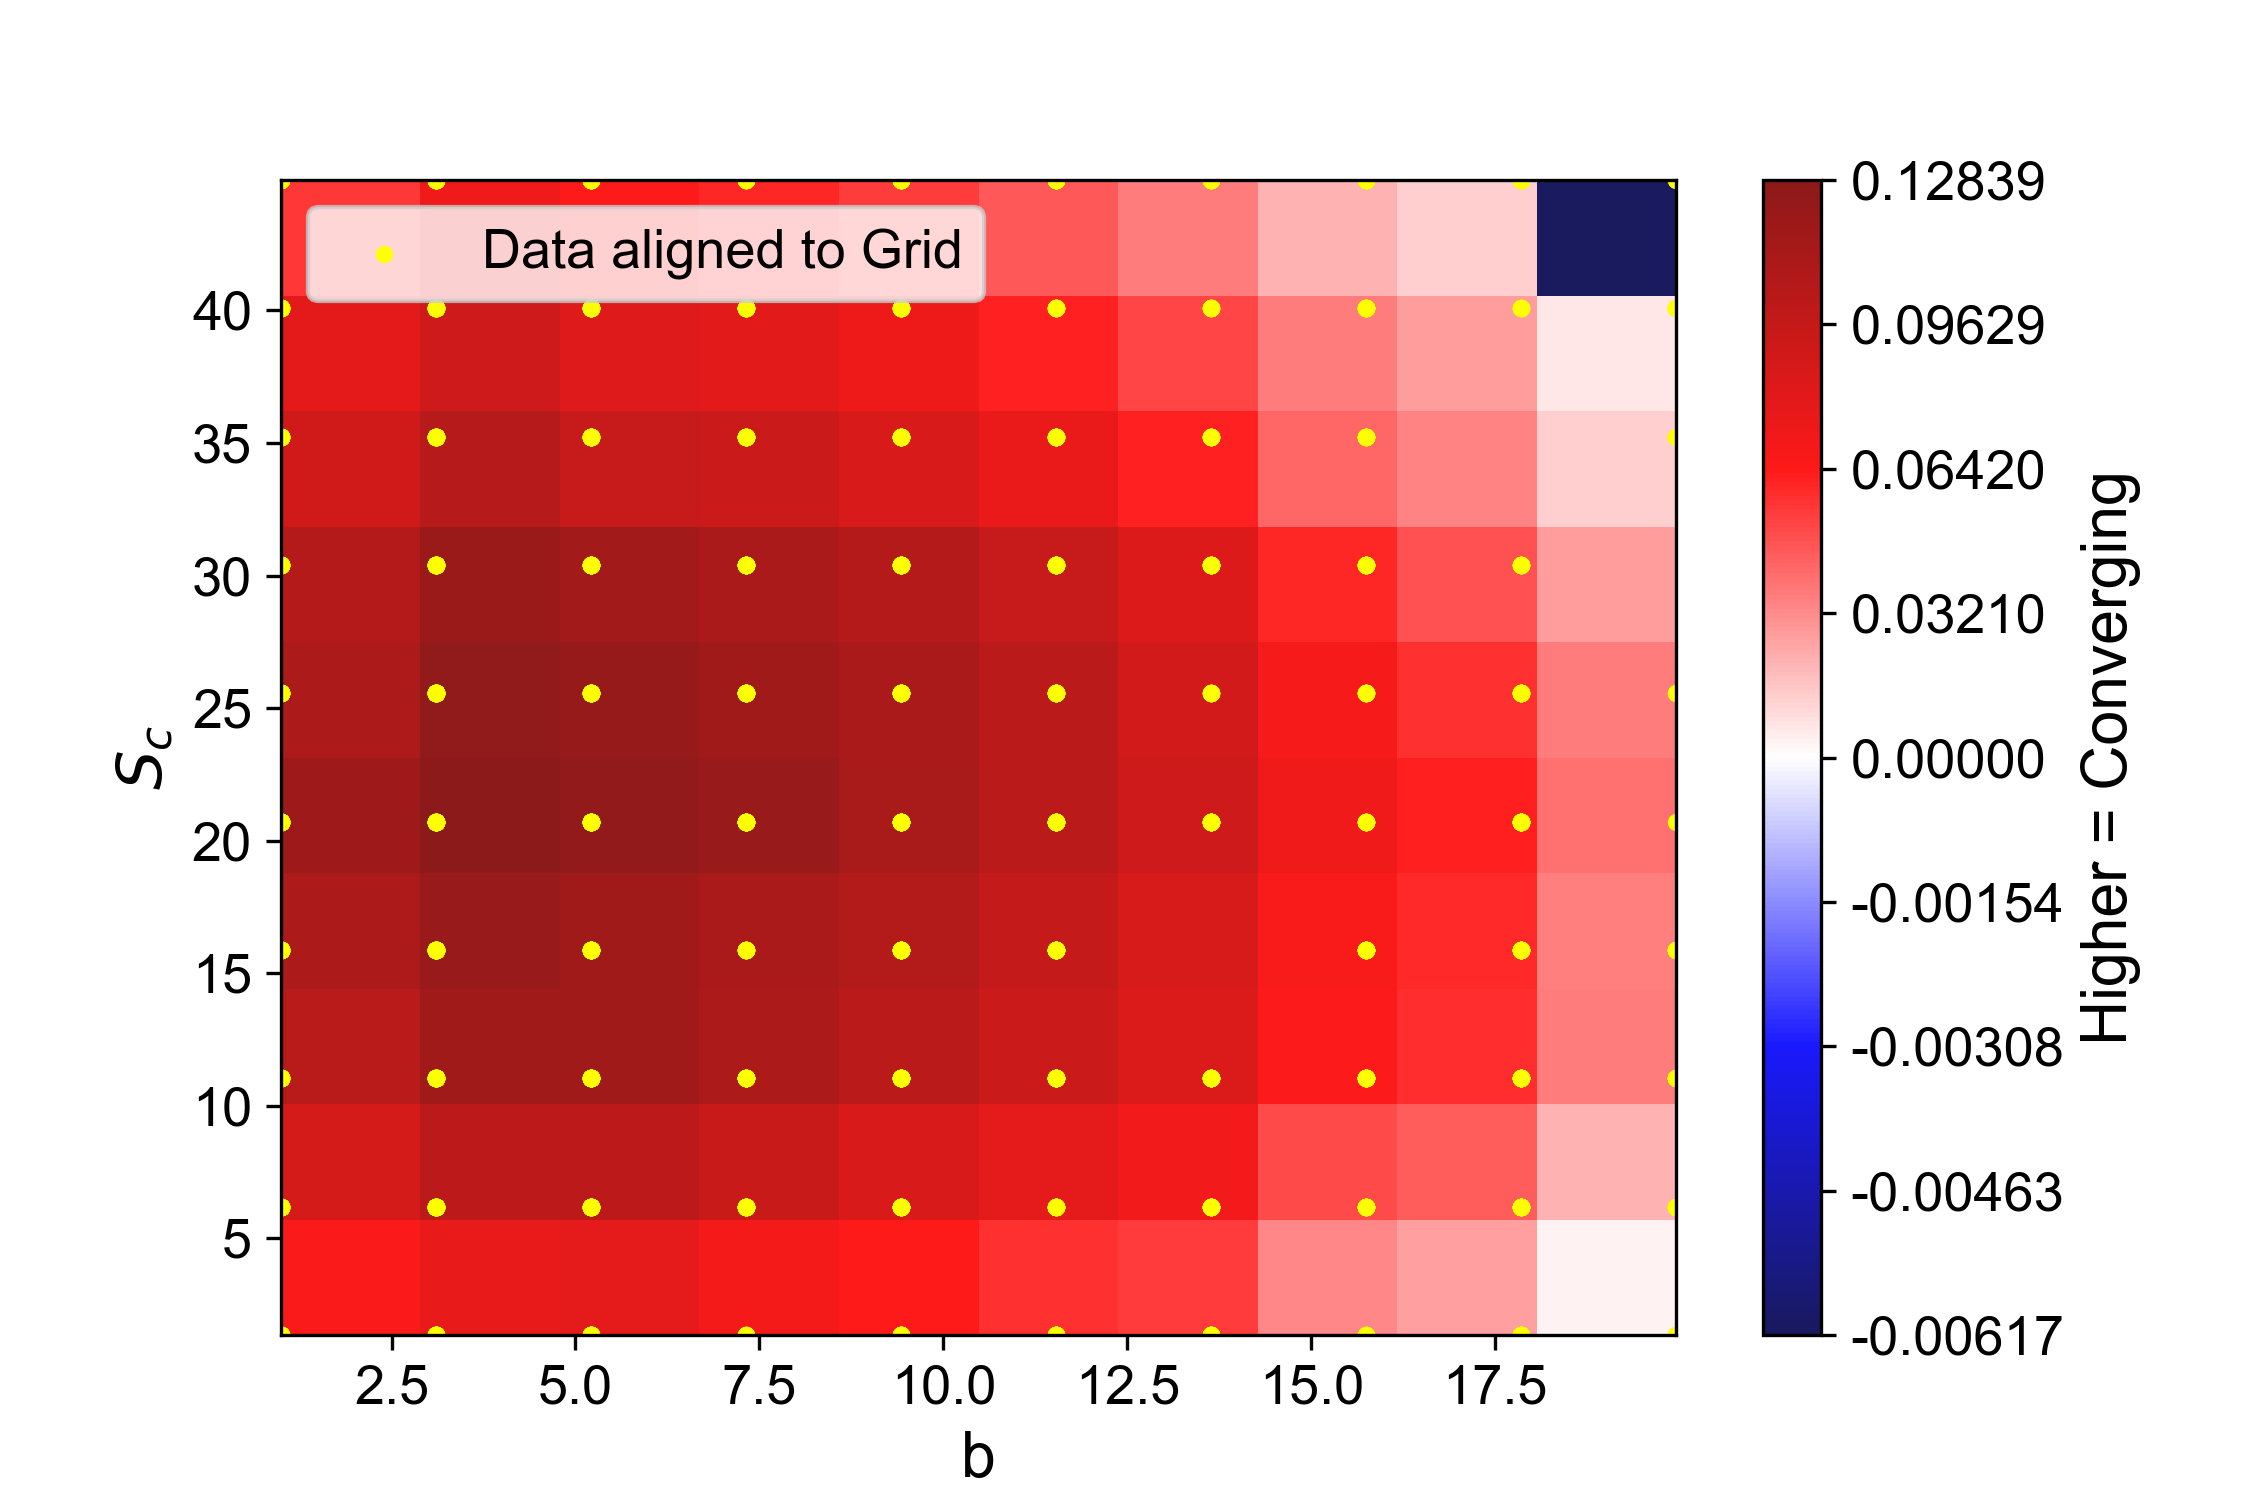
\includegraphics[width=0.32\textwidth]{figures/convergence/pairwise_projections_4.png} &
			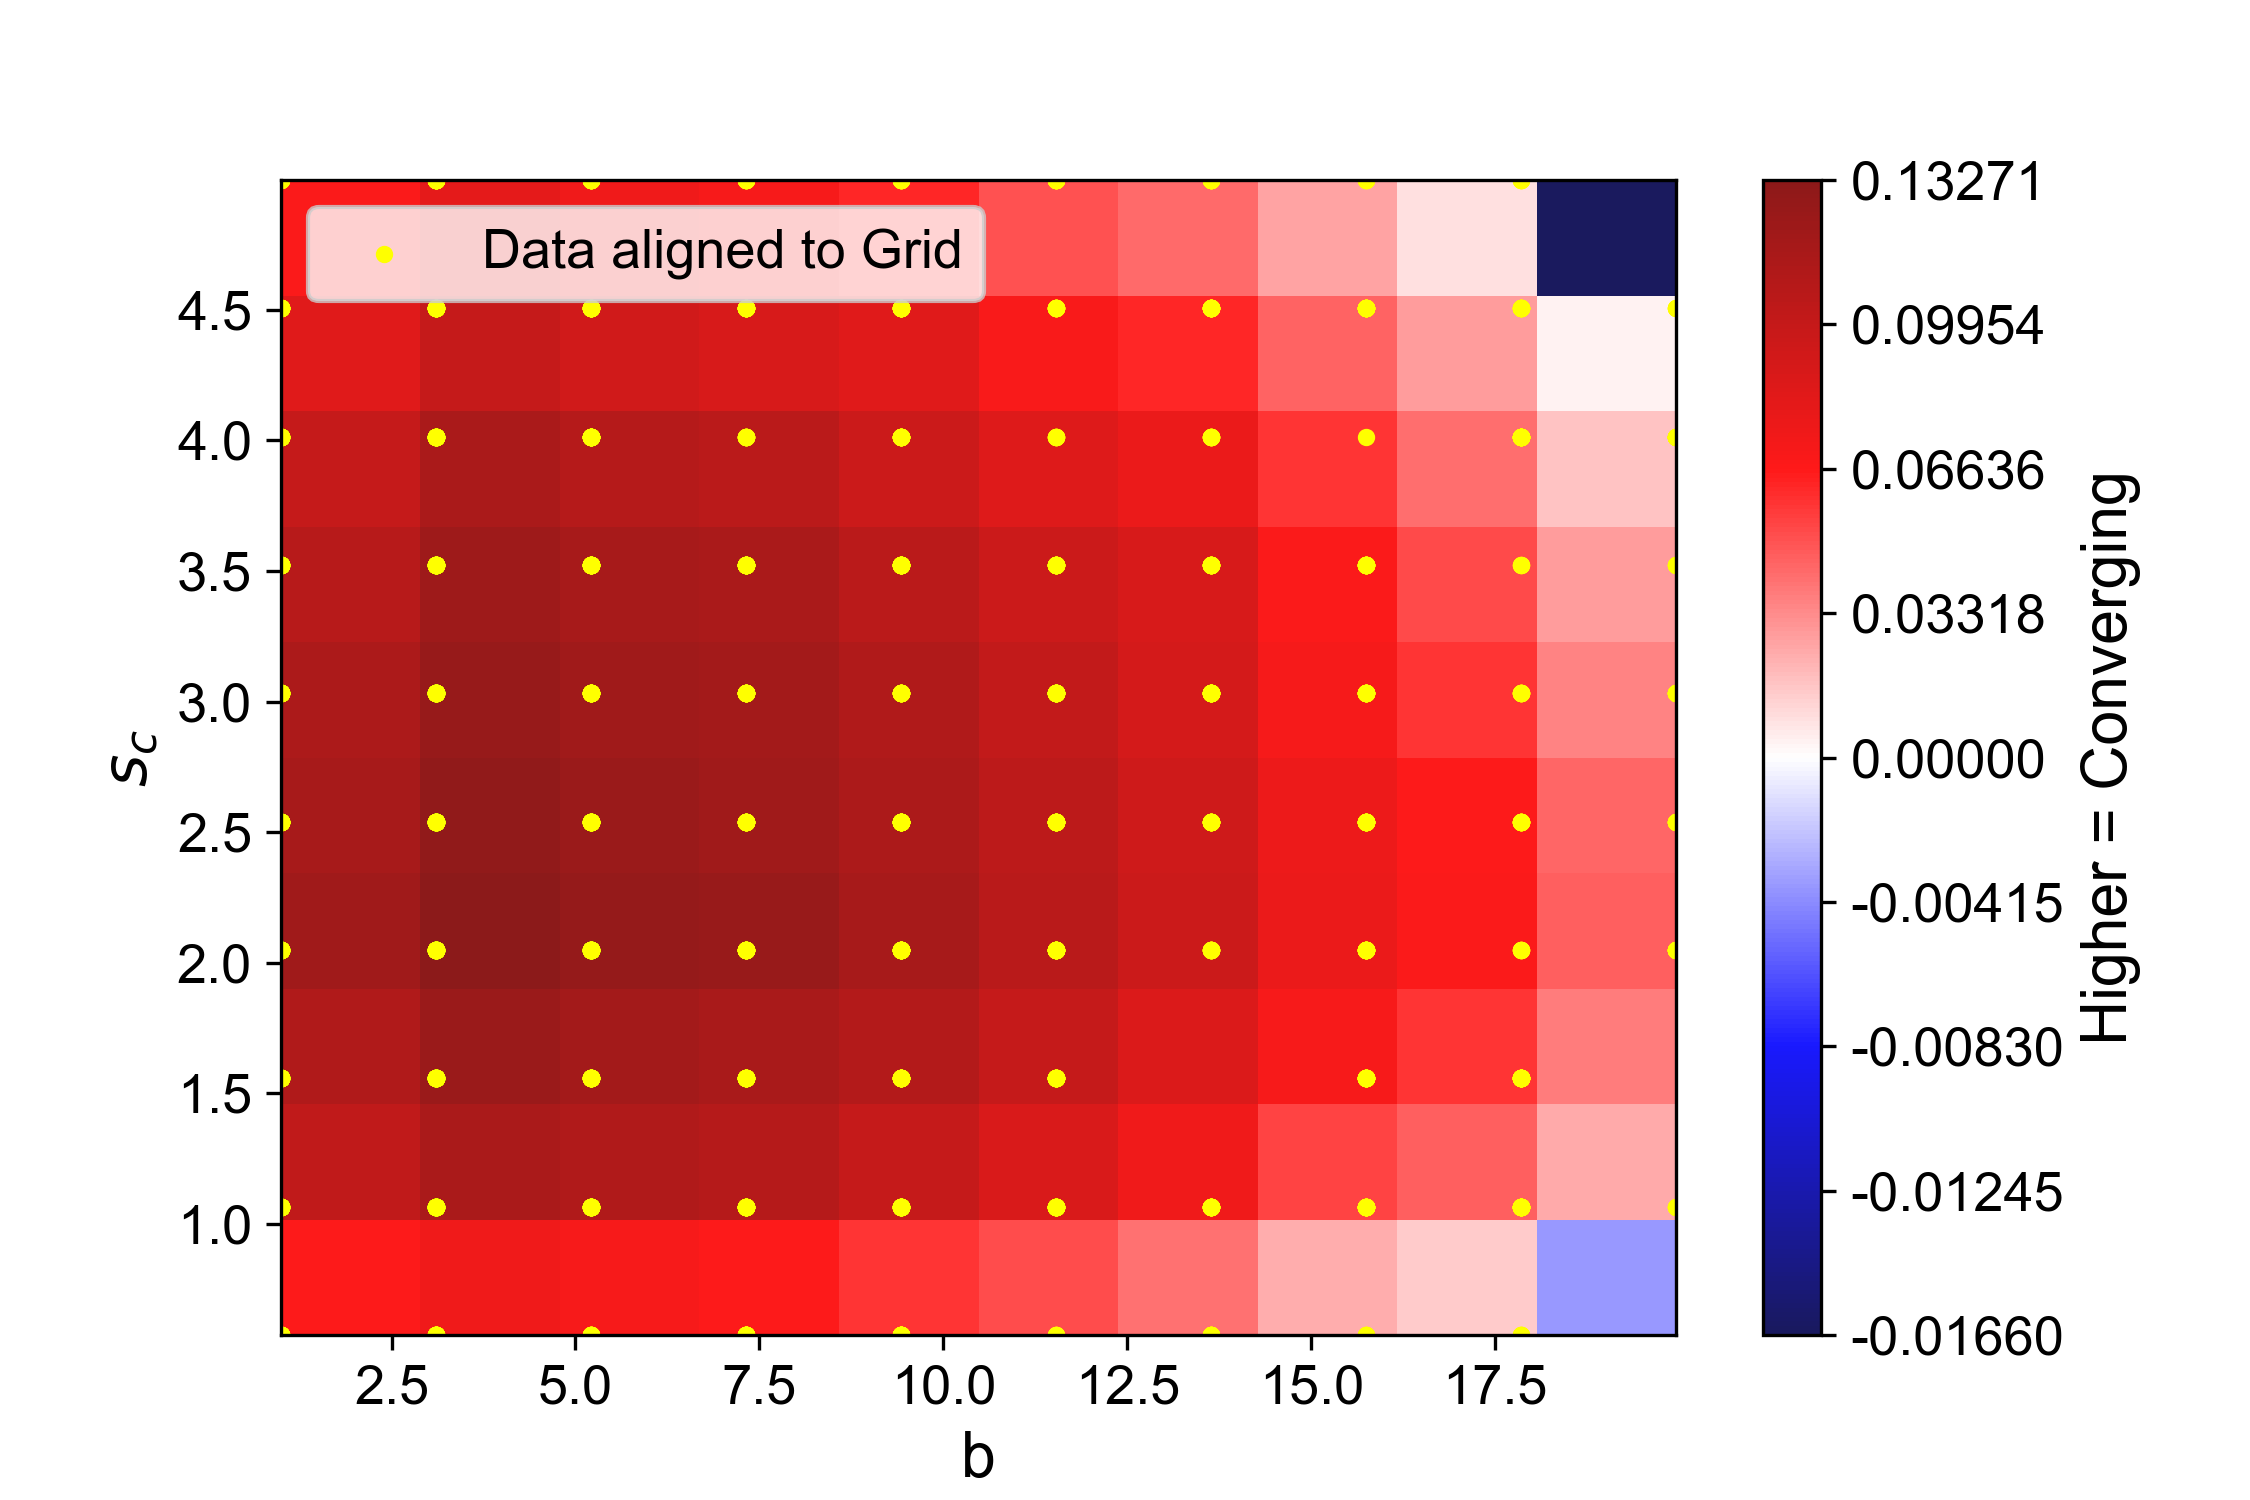
\includegraphics[width=0.32\textwidth]{figures/convergence/pairwise_projections_5.png} &
			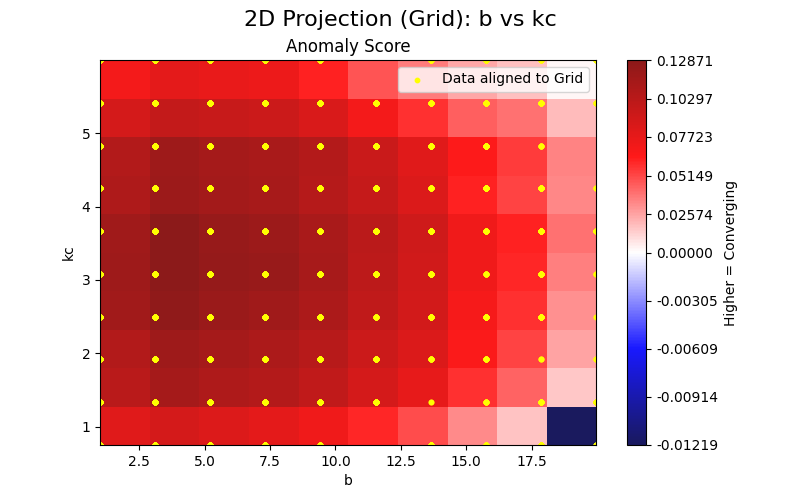
\includegraphics[width=0.32\textwidth]{figures/convergence/pairwise_projections_6.png} \\
			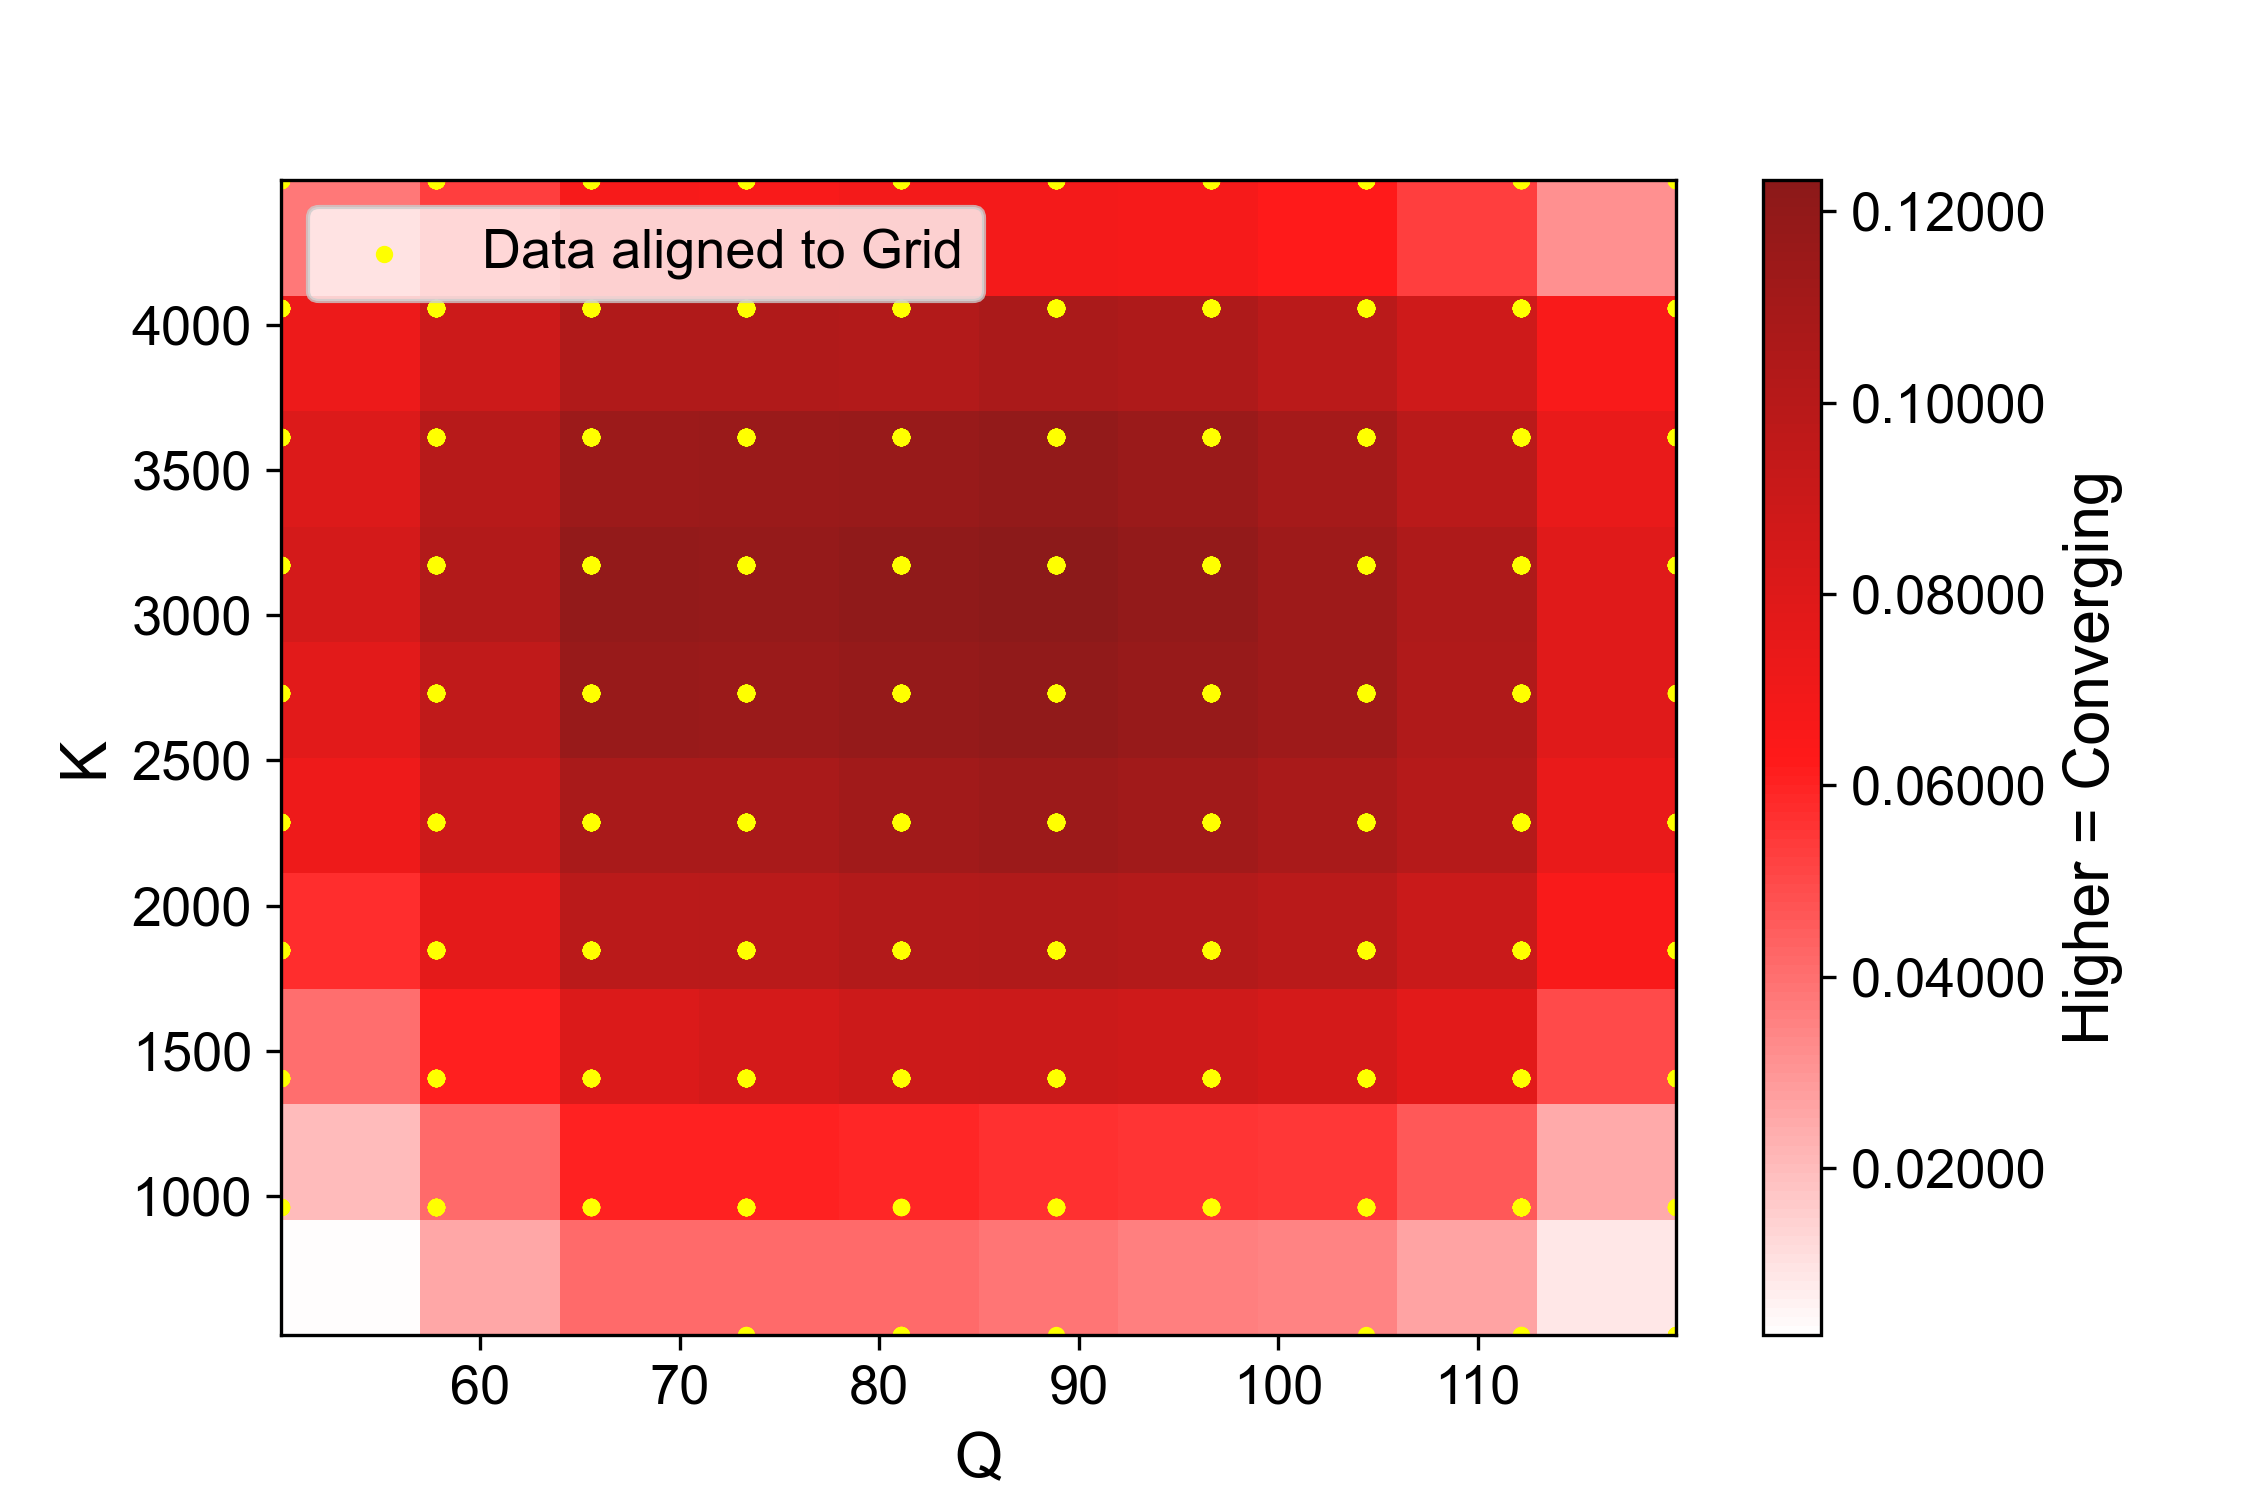
\includegraphics[width=0.32\textwidth]{figures/convergence/pairwise_projections_7.png} &
			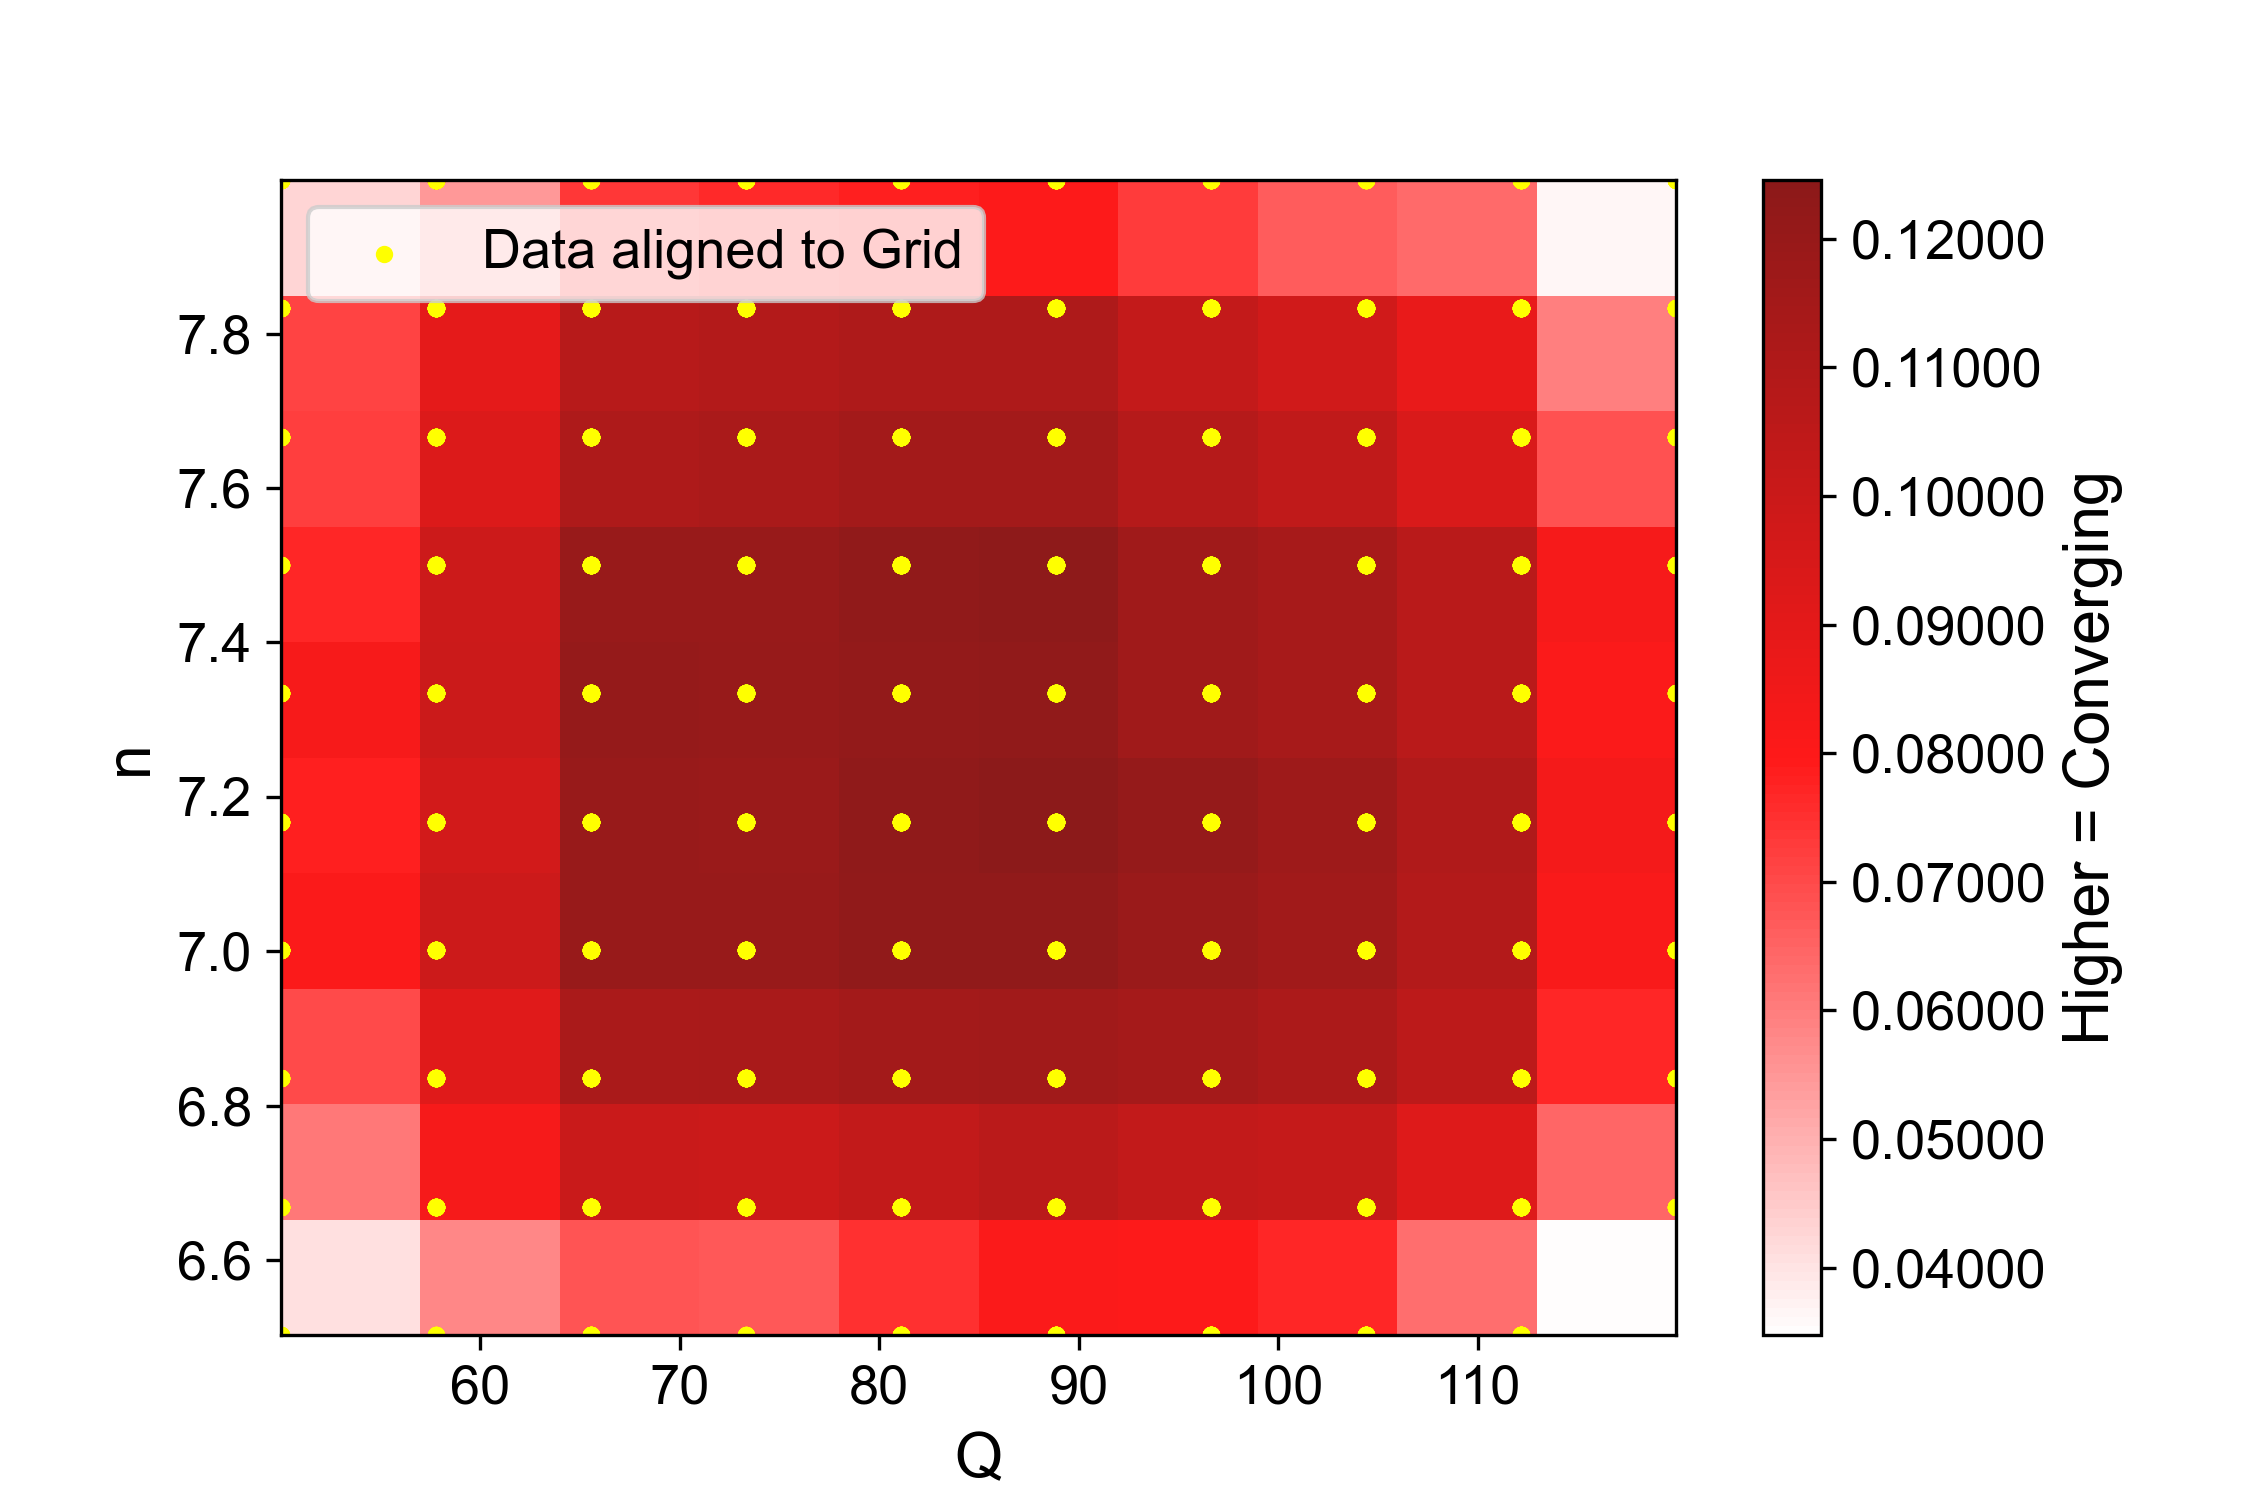
\includegraphics[width=0.32\textwidth]{figures/convergence/pairwise_projections_8.png} &
			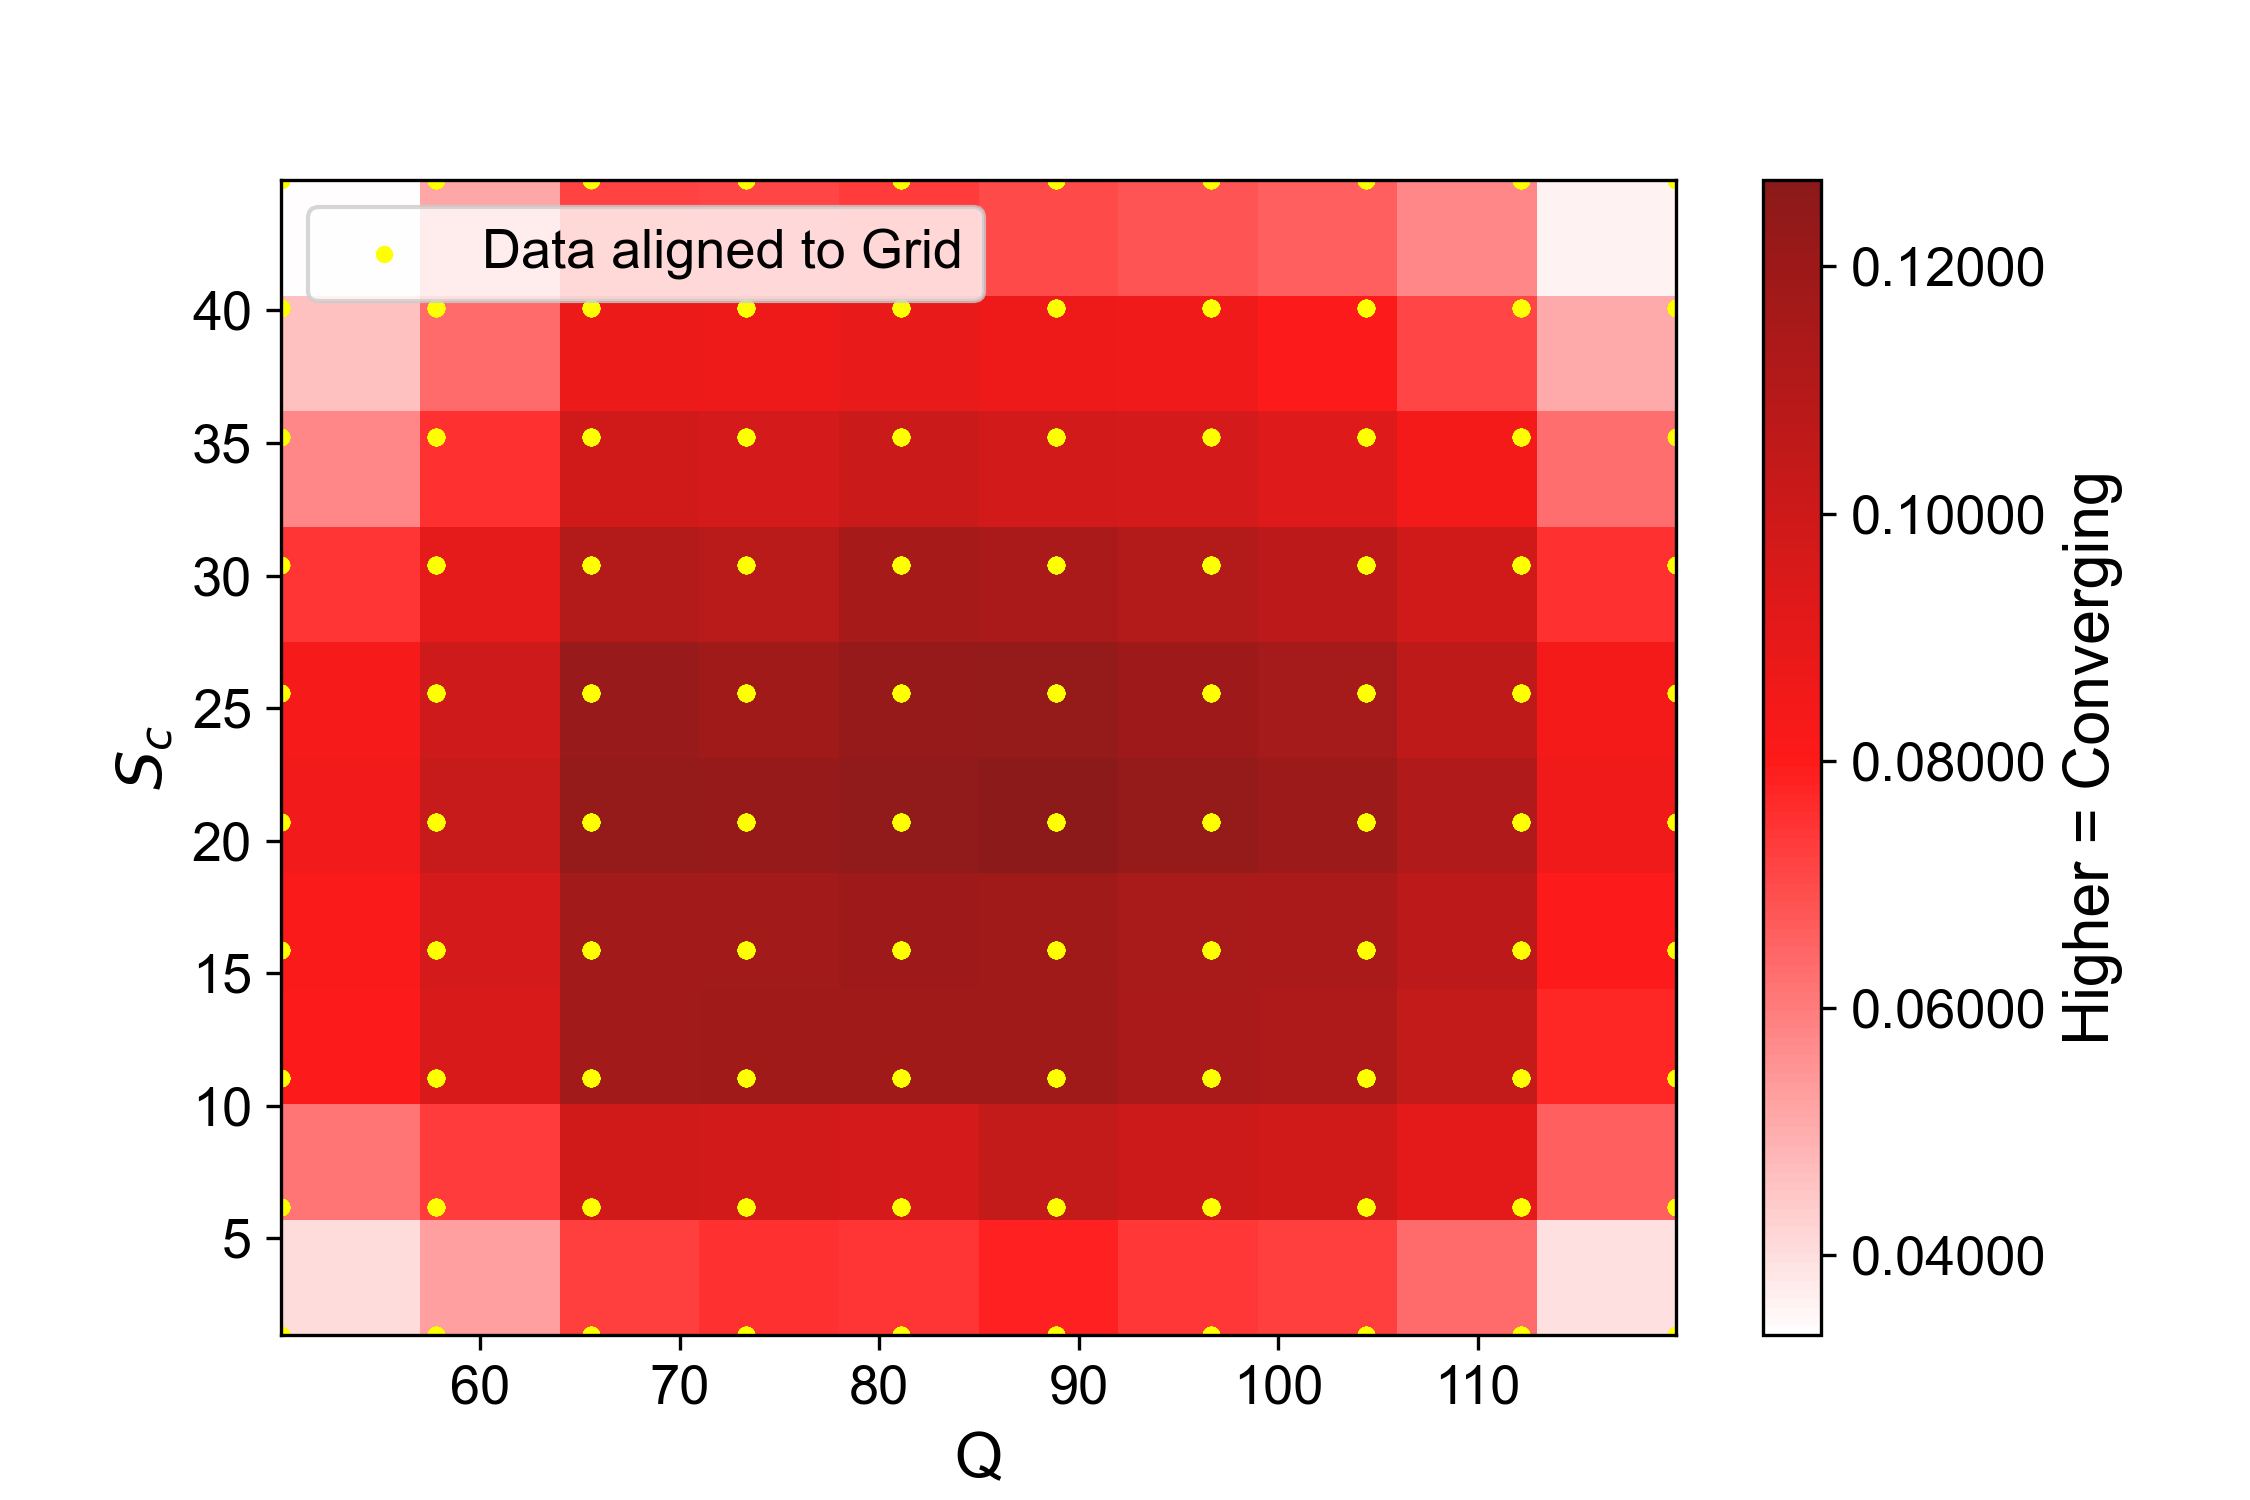
\includegraphics[width=0.32\textwidth]{figures/convergence/pairwise_projections_9.png} \\
			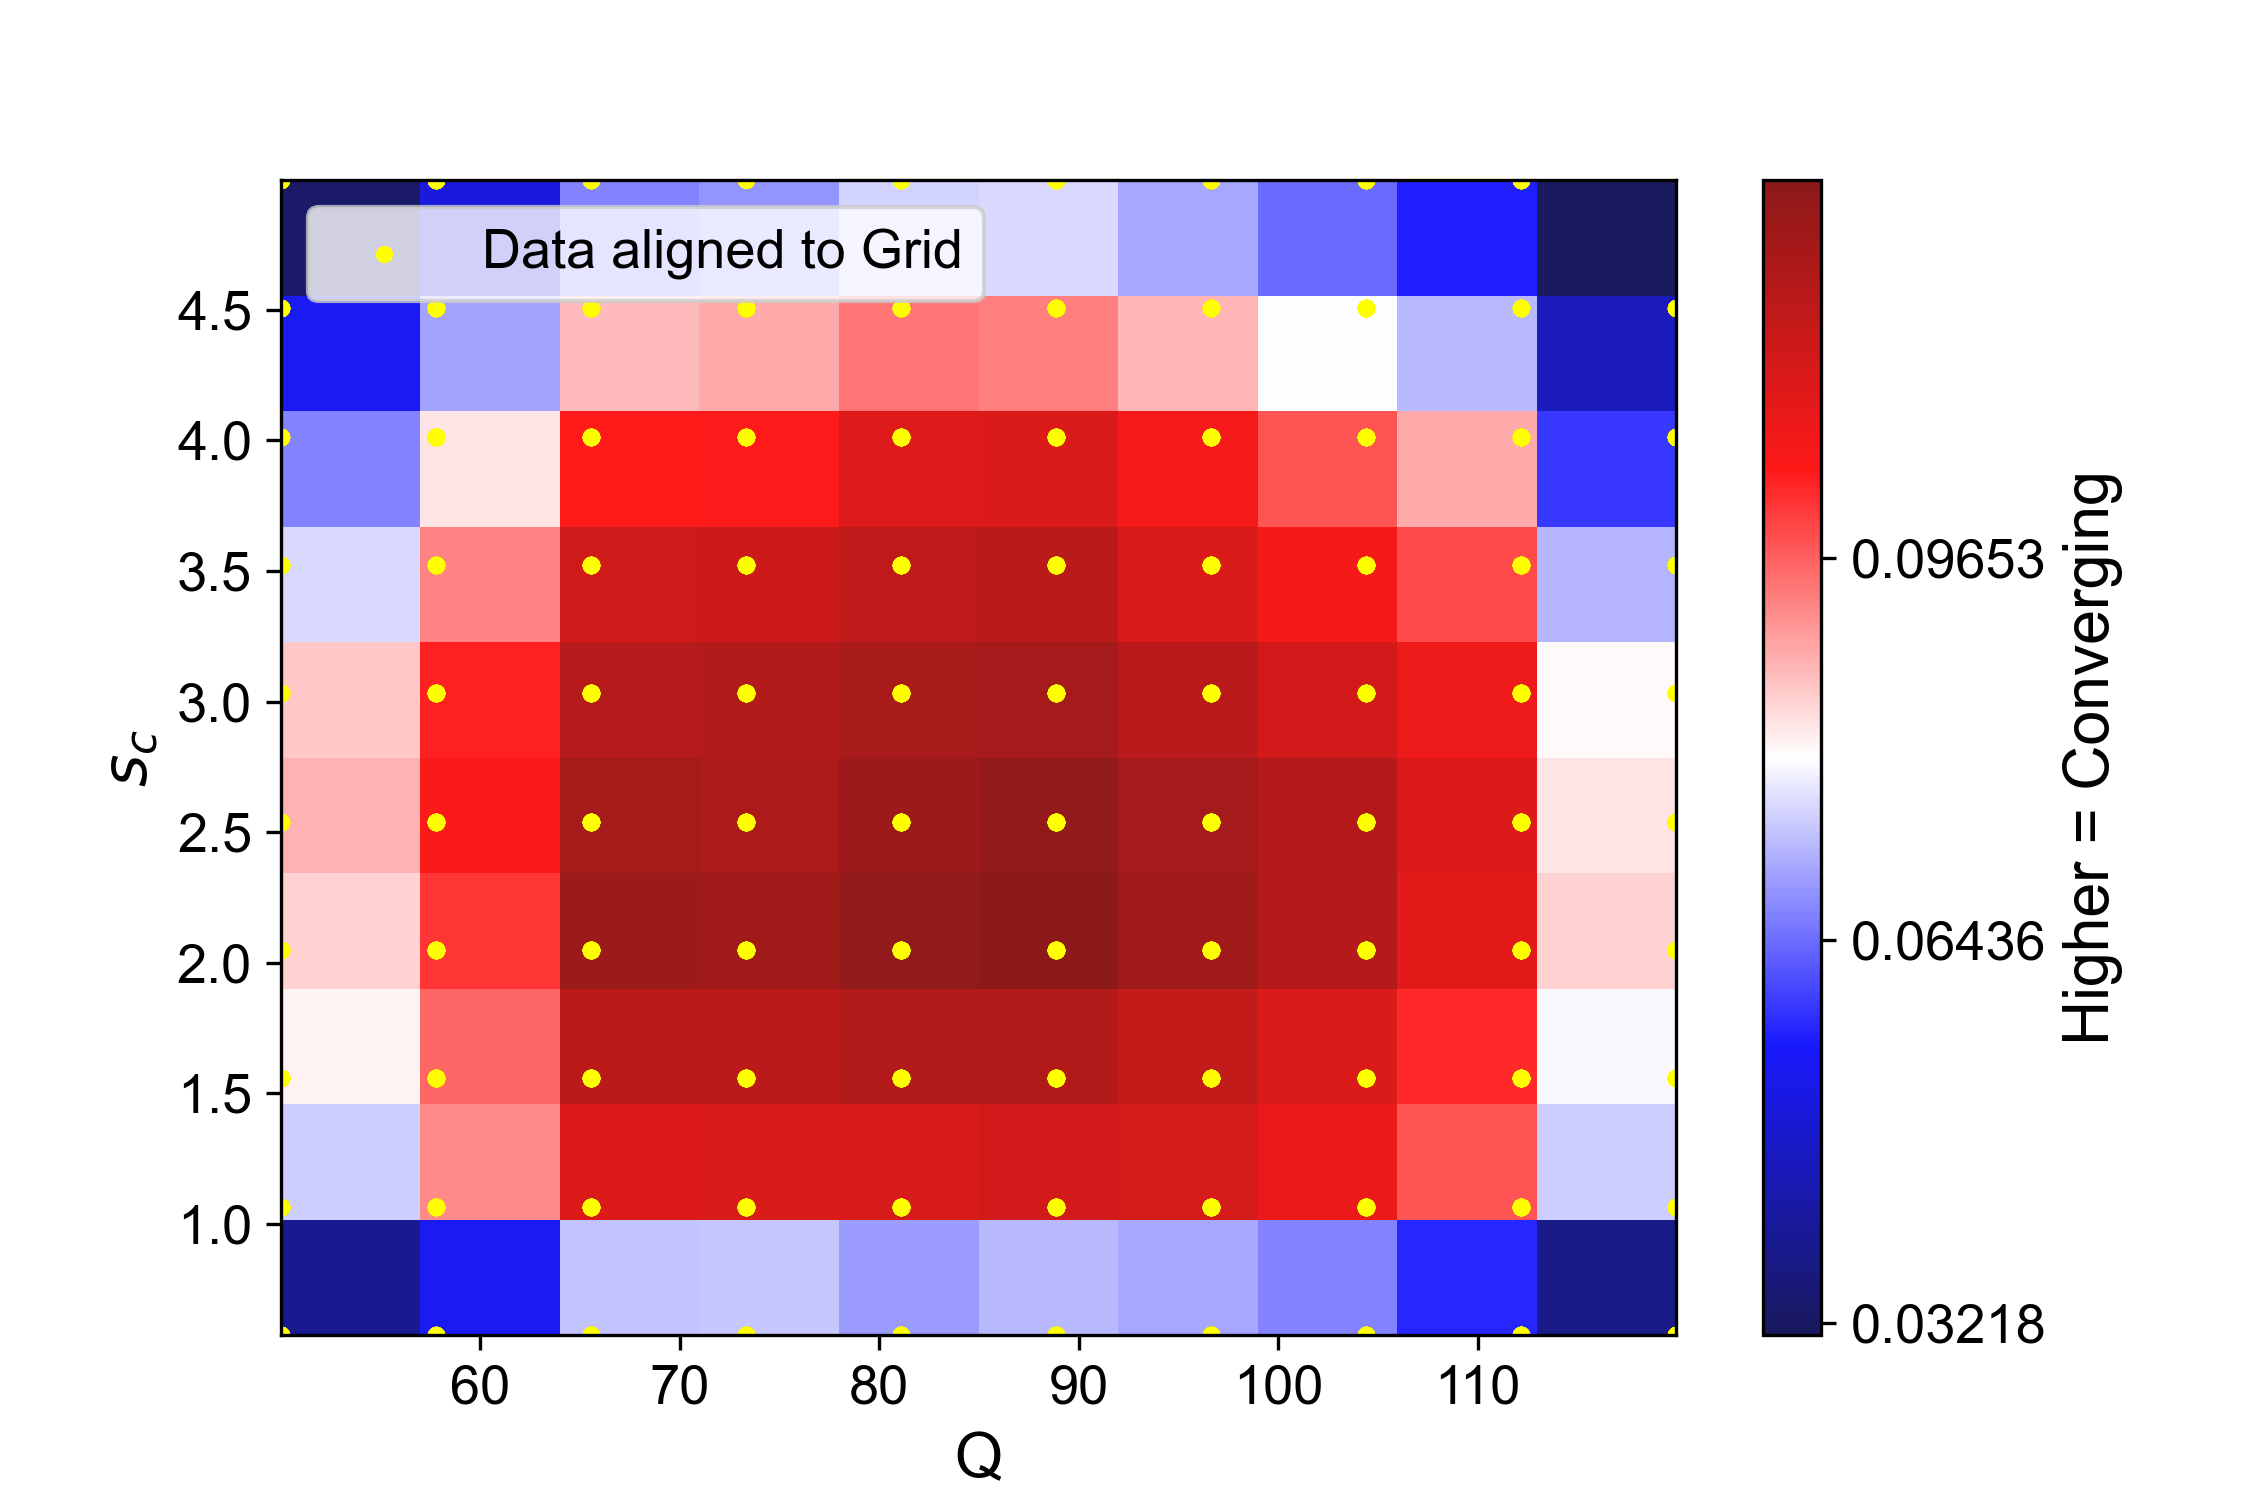
\includegraphics[width=0.32\textwidth]{figures/convergence/pairwise_projections_10.png} &
			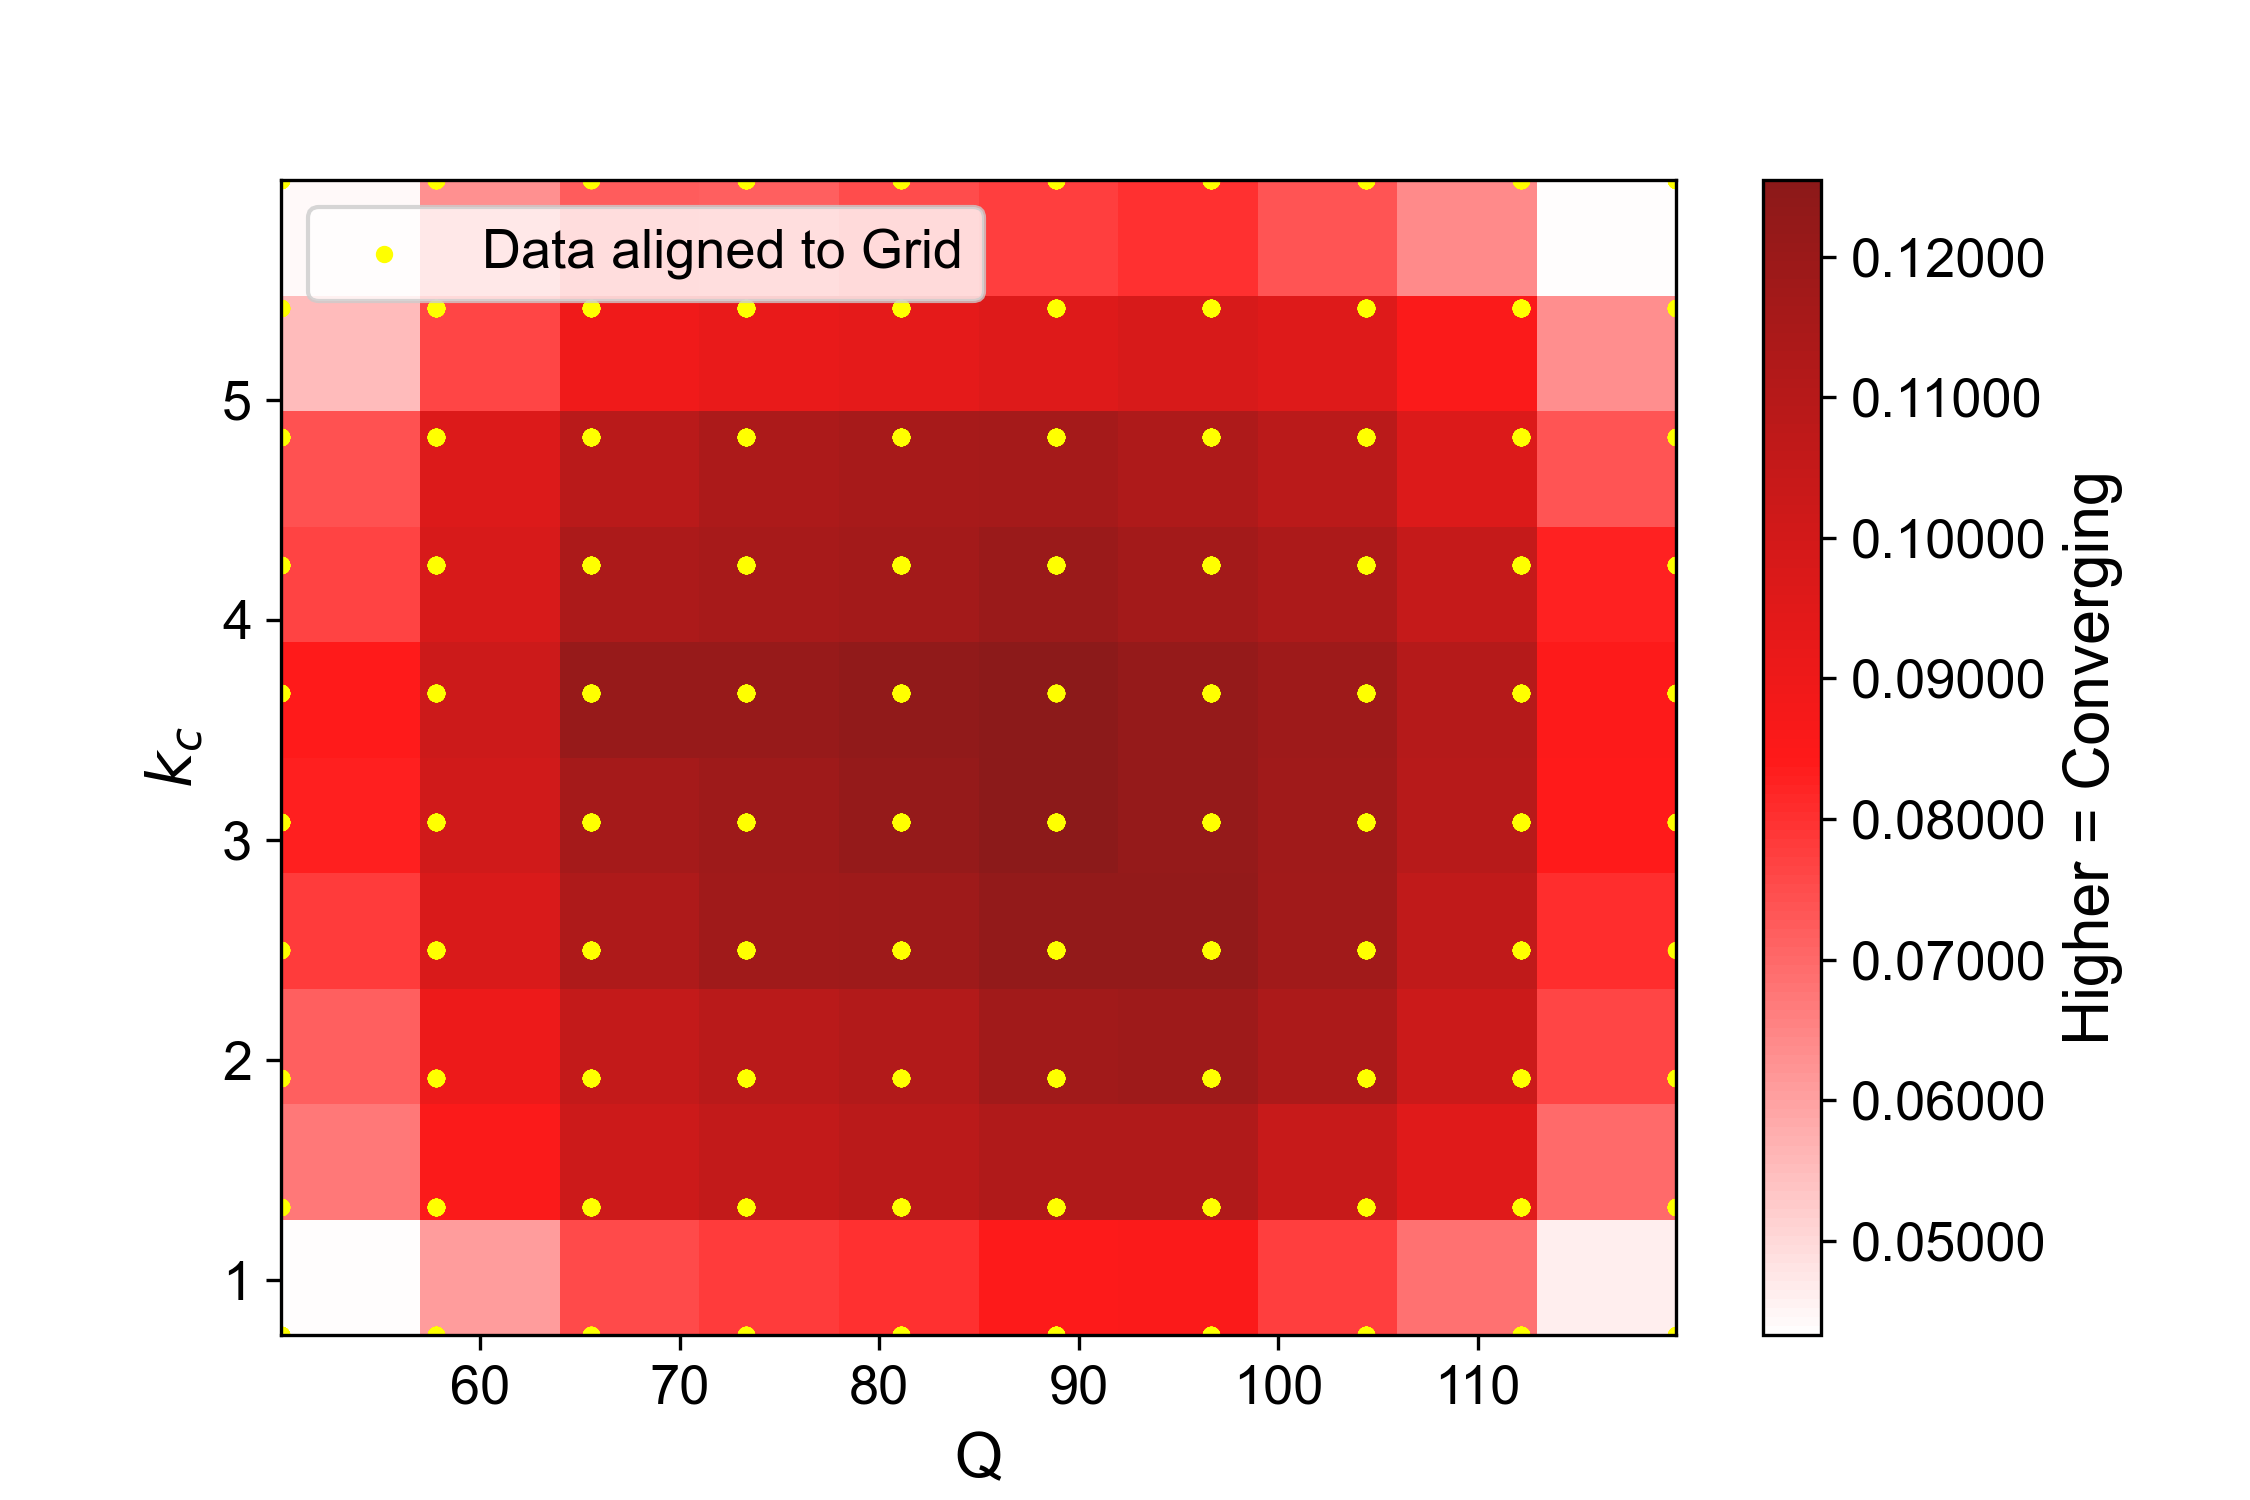
\includegraphics[width=0.32\textwidth]{figures/convergence/pairwise_projections_11.png} &
			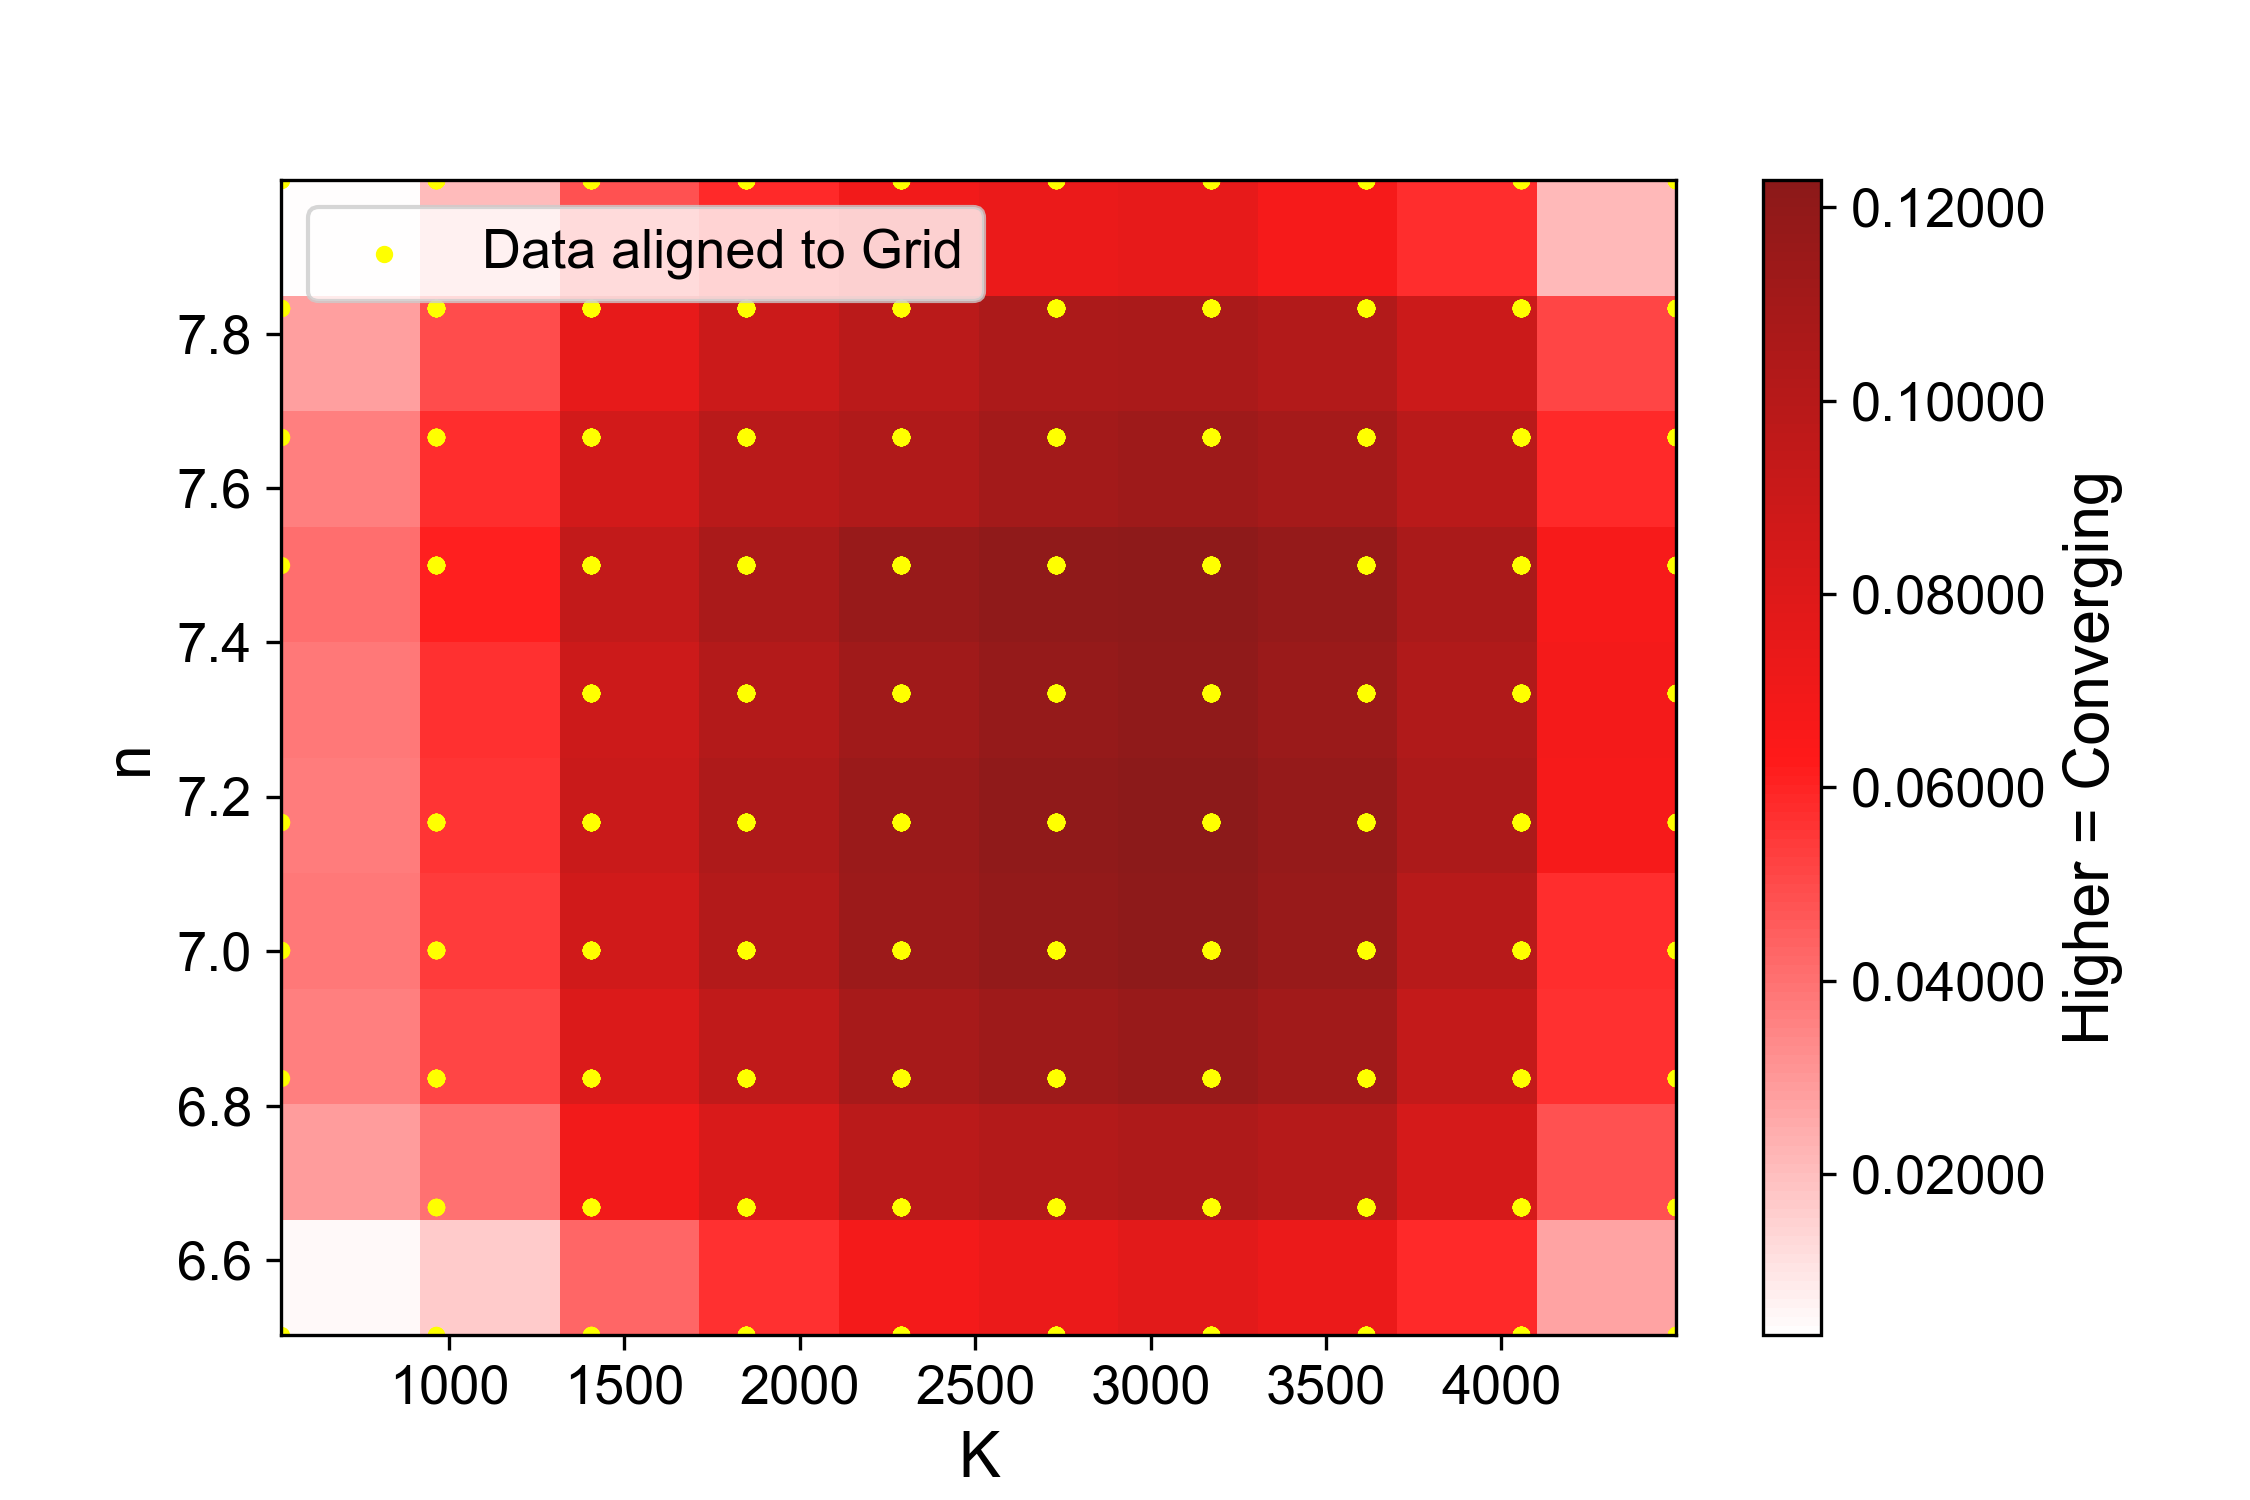
\includegraphics[width=0.32\textwidth]{figures/convergence/pairwise_projections_12.png} \\
			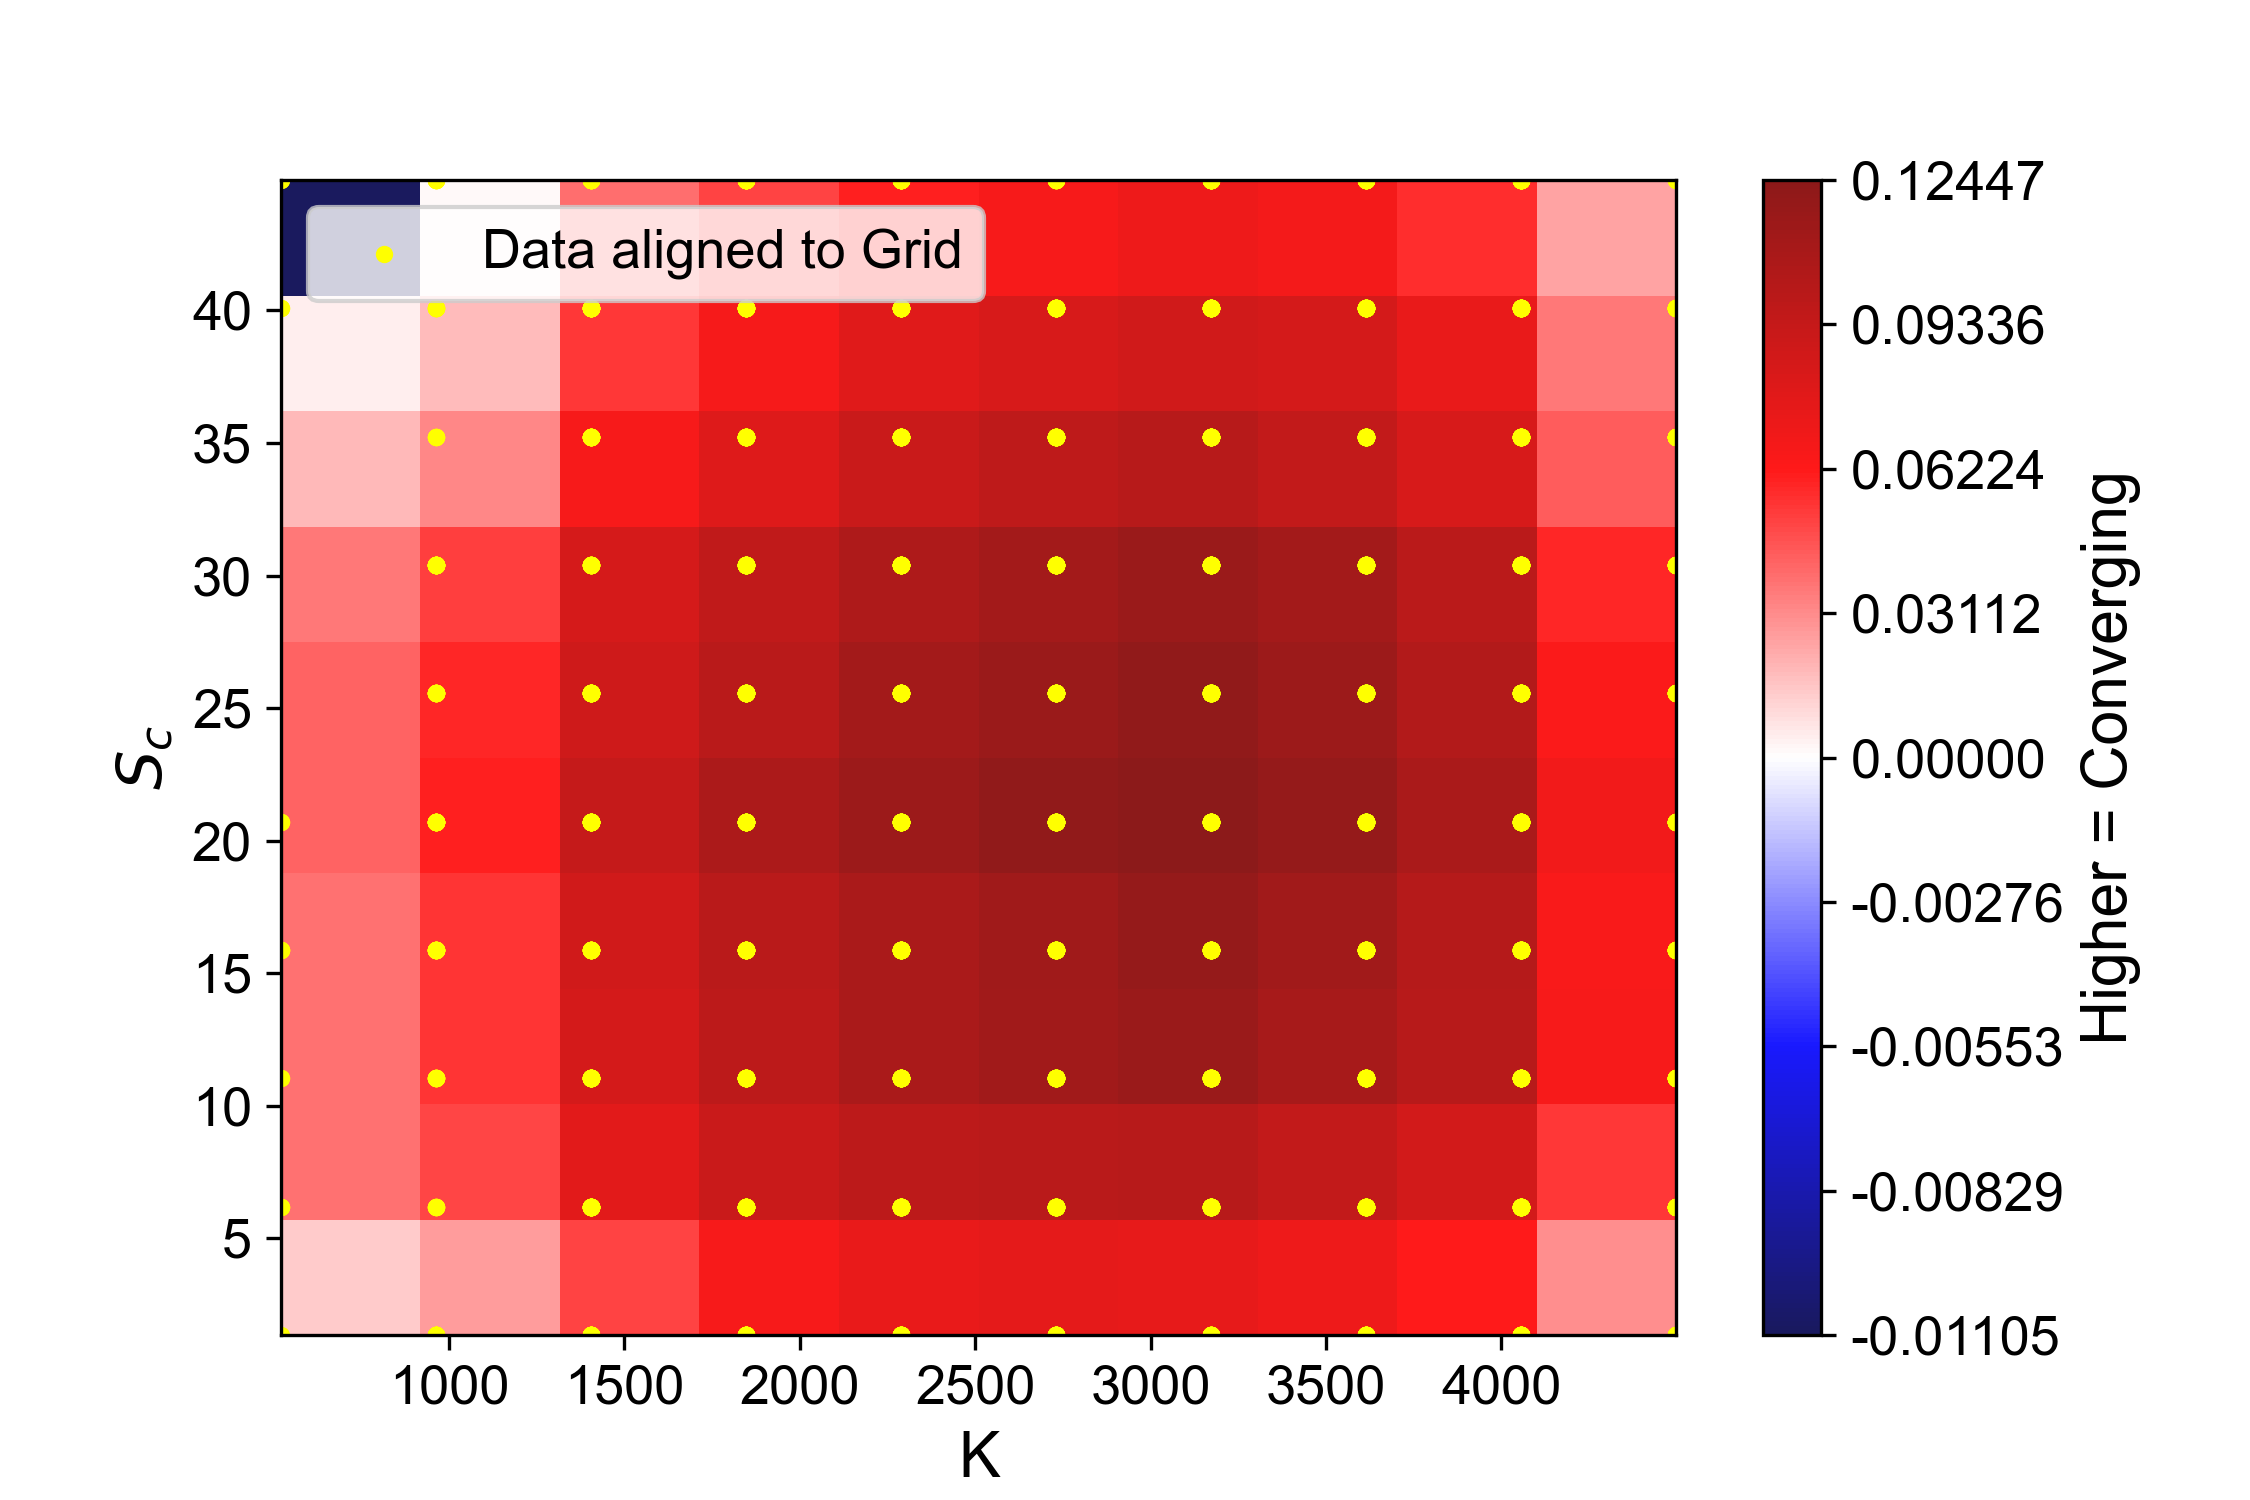
\includegraphics[width=0.32\textwidth]{figures/convergence/pairwise_projections_13.png} &
			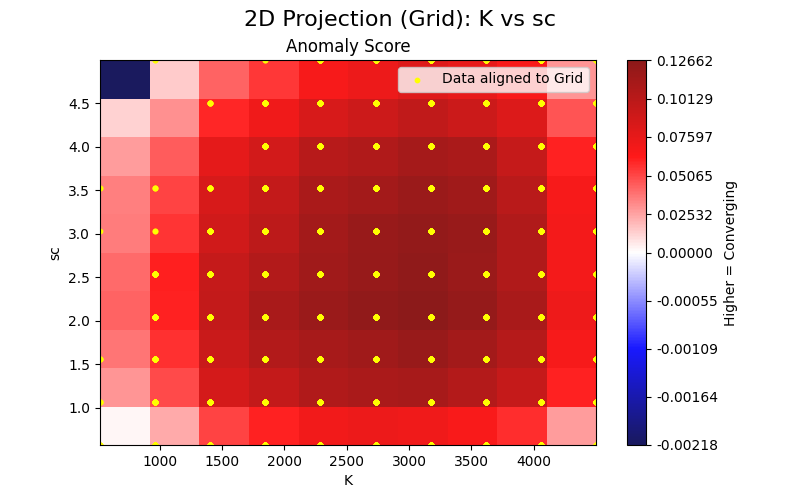
\includegraphics[width=0.32\textwidth]{figures/convergence/pairwise_projections_14.png} &
			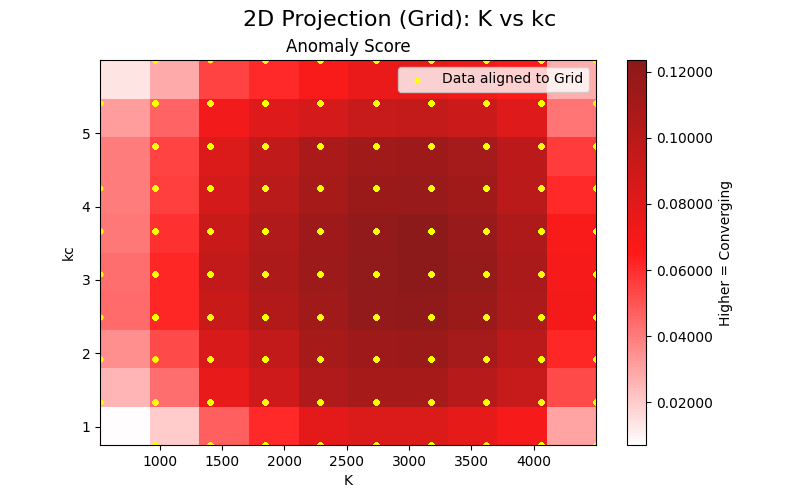
\includegraphics[width=0.32\textwidth]{figures/convergence/pairwise_projections_15.png} \\
			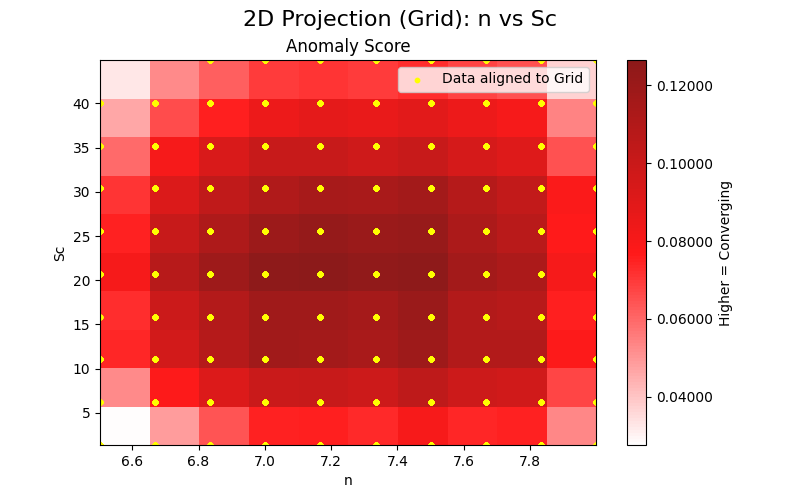
\includegraphics[width=0.32\textwidth]{figures/convergence/pairwise_projections_16.png} &
			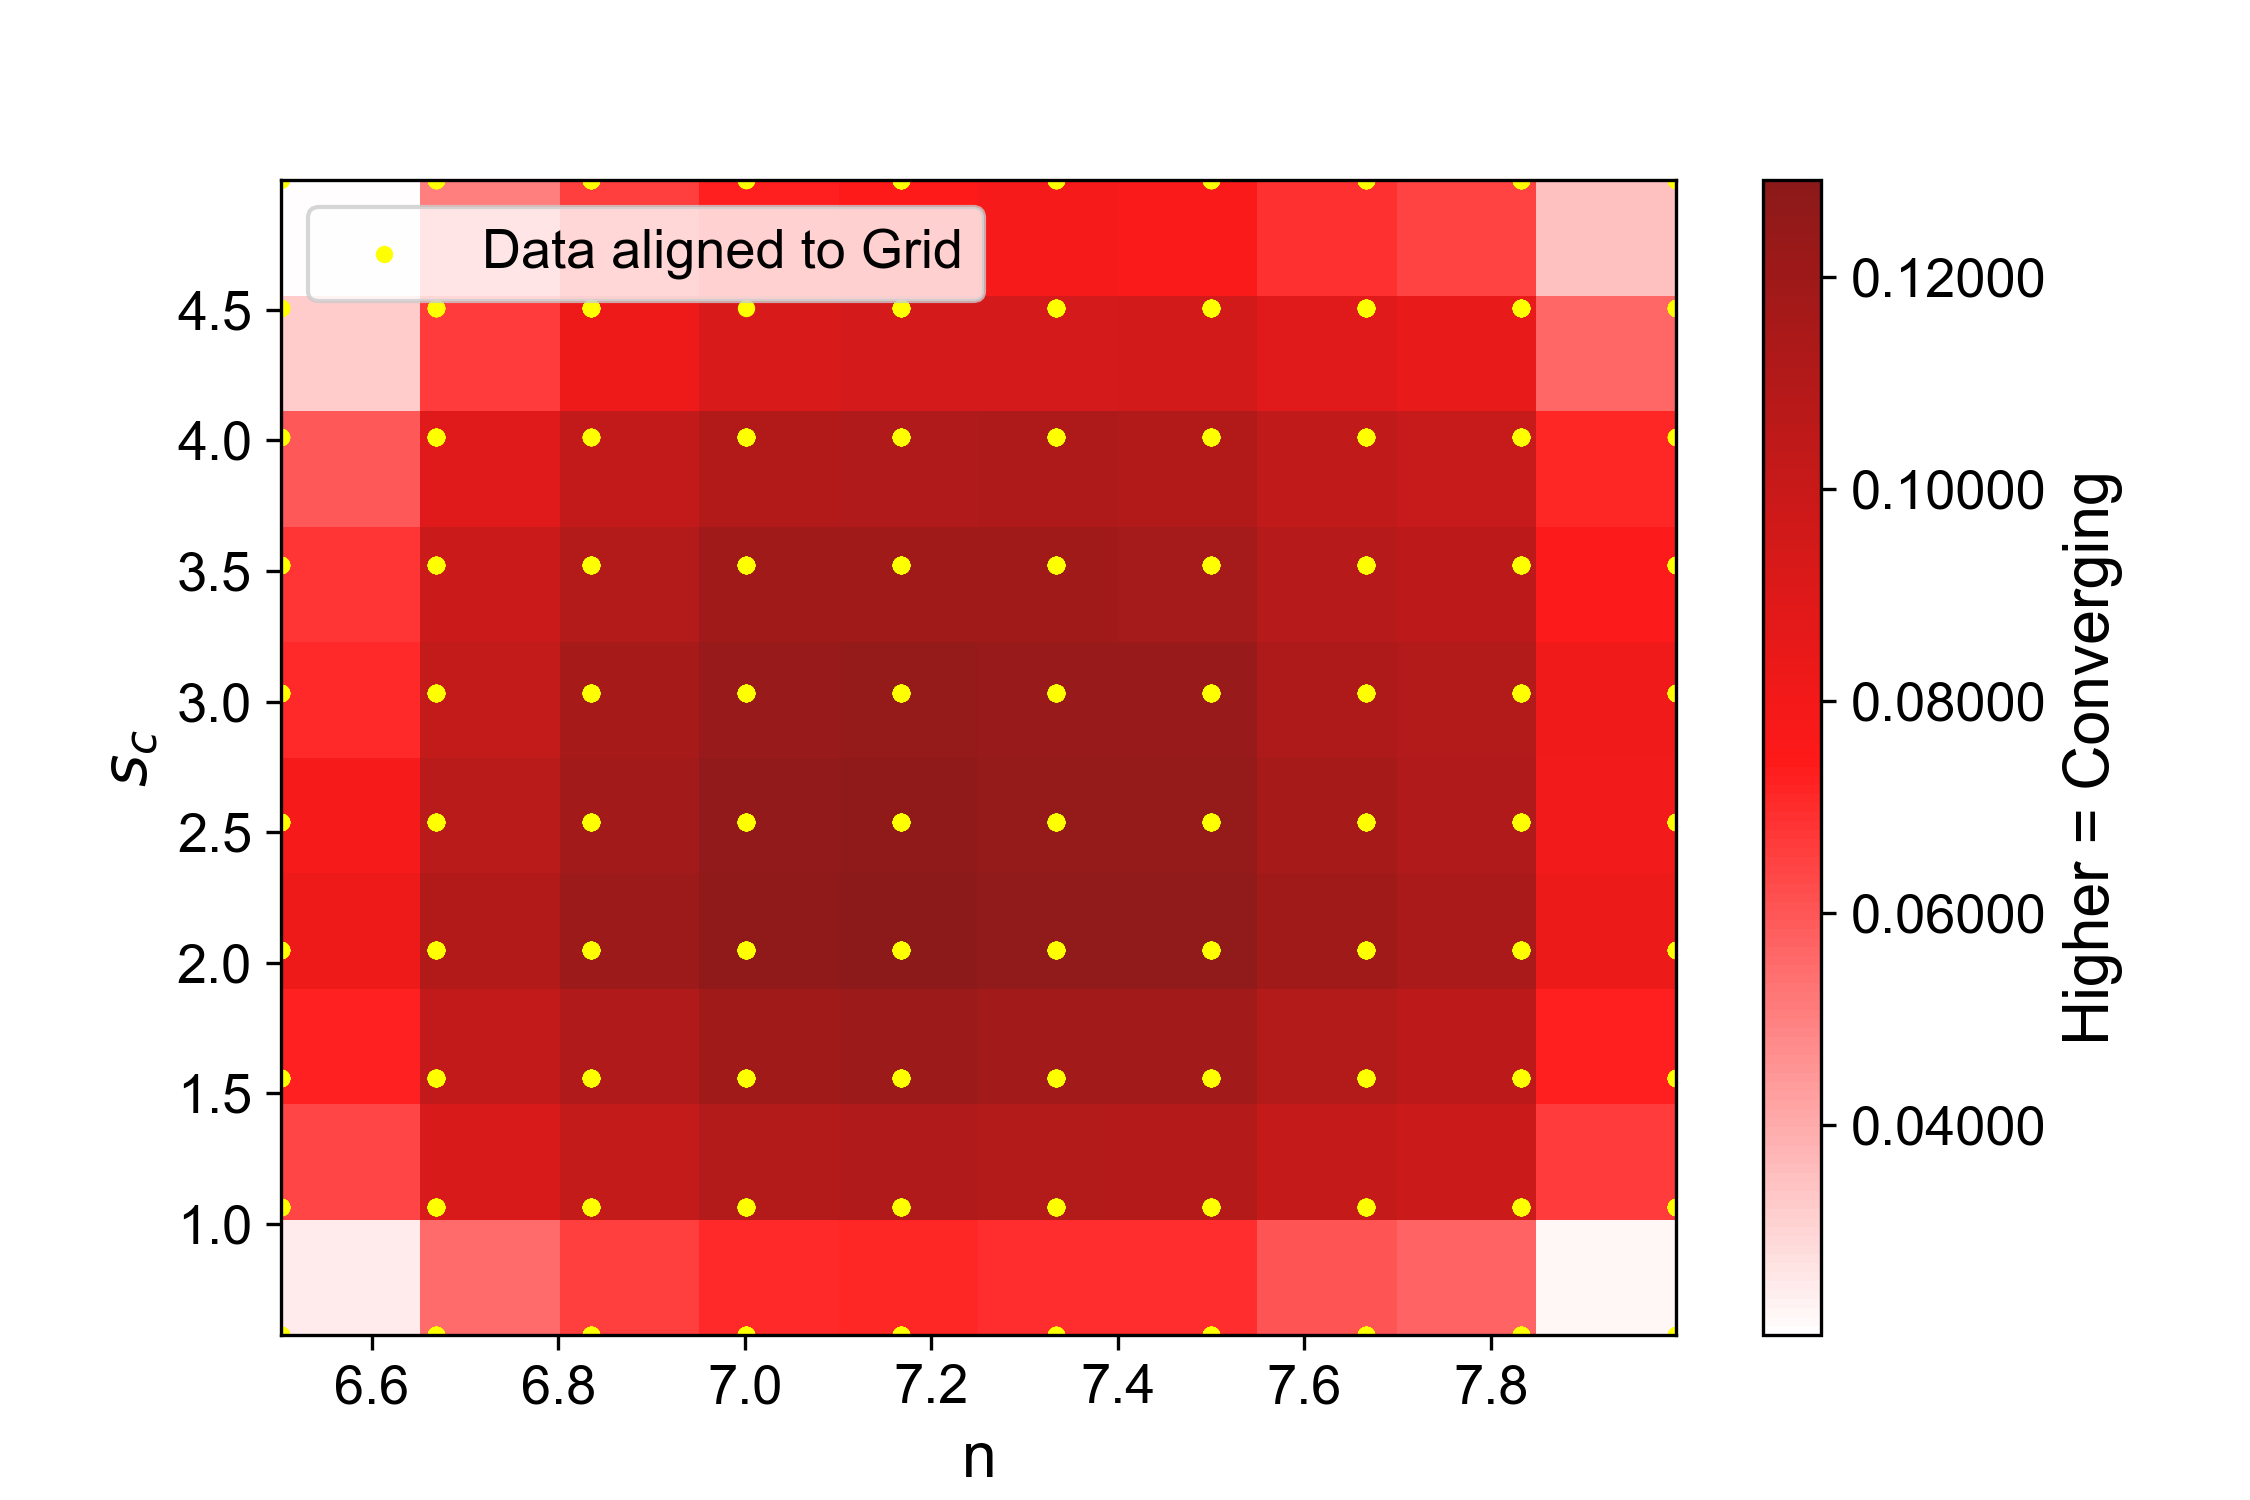
\includegraphics[width=0.32\textwidth]{figures/convergence/pairwise_projections_17.png} &
			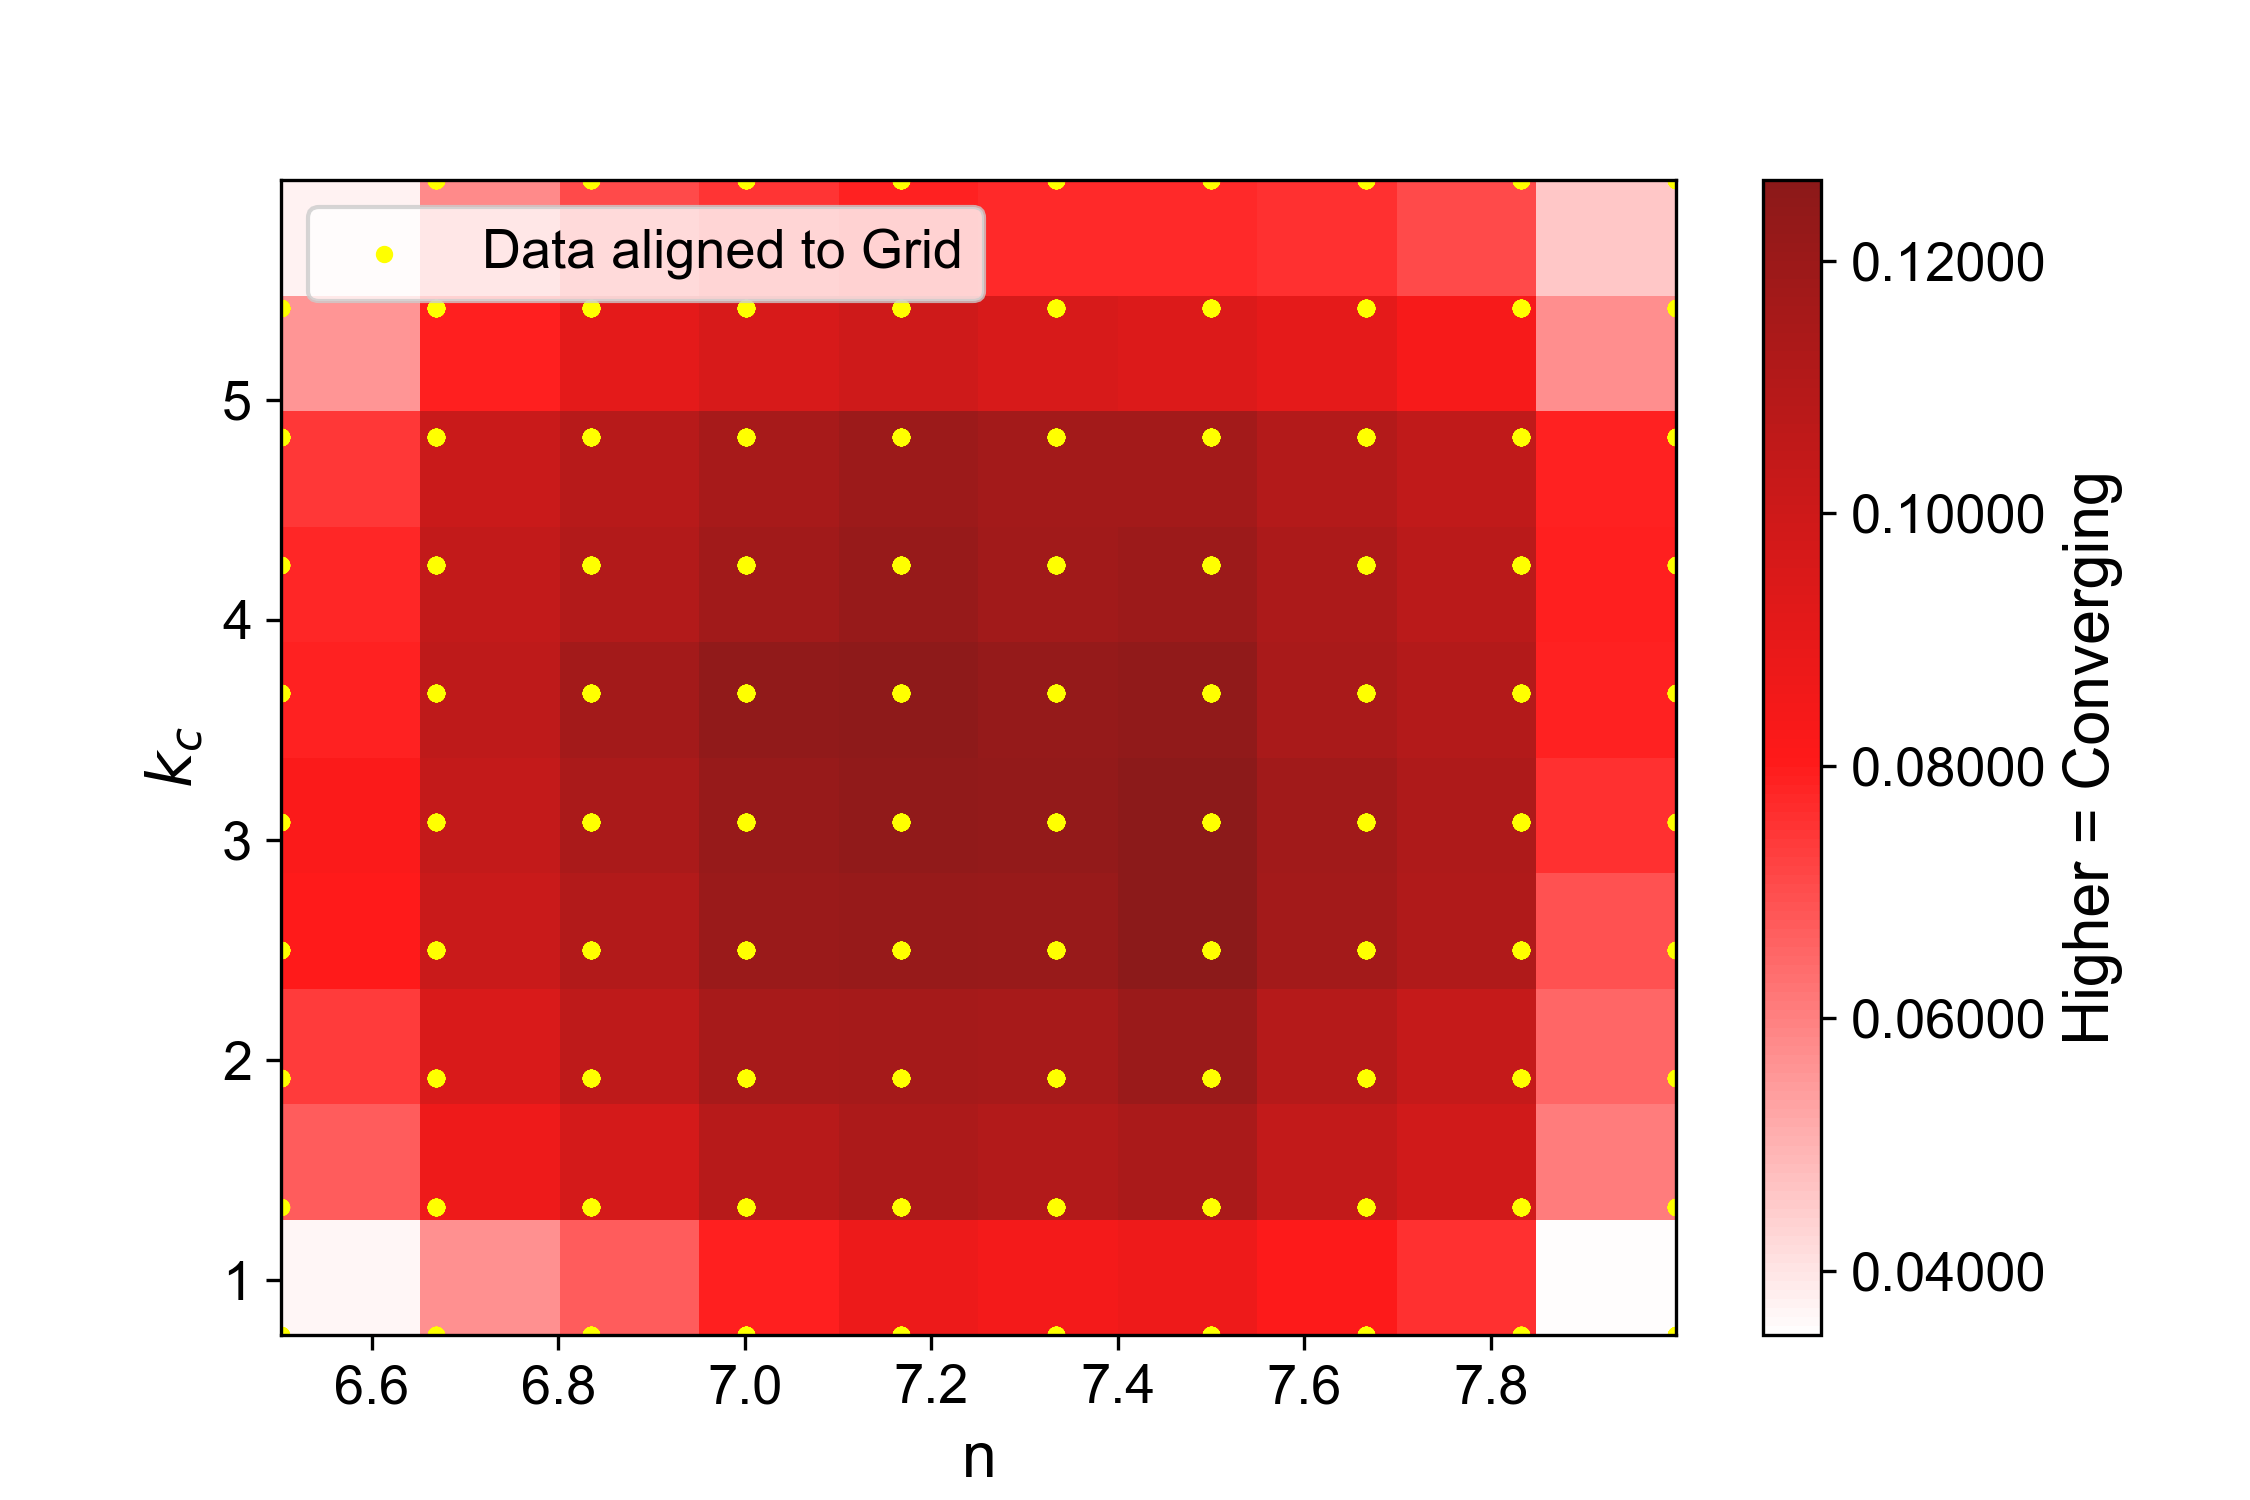
\includegraphics[width=0.32\textwidth]{figures/convergence/pairwise_projections_18.png} \\
			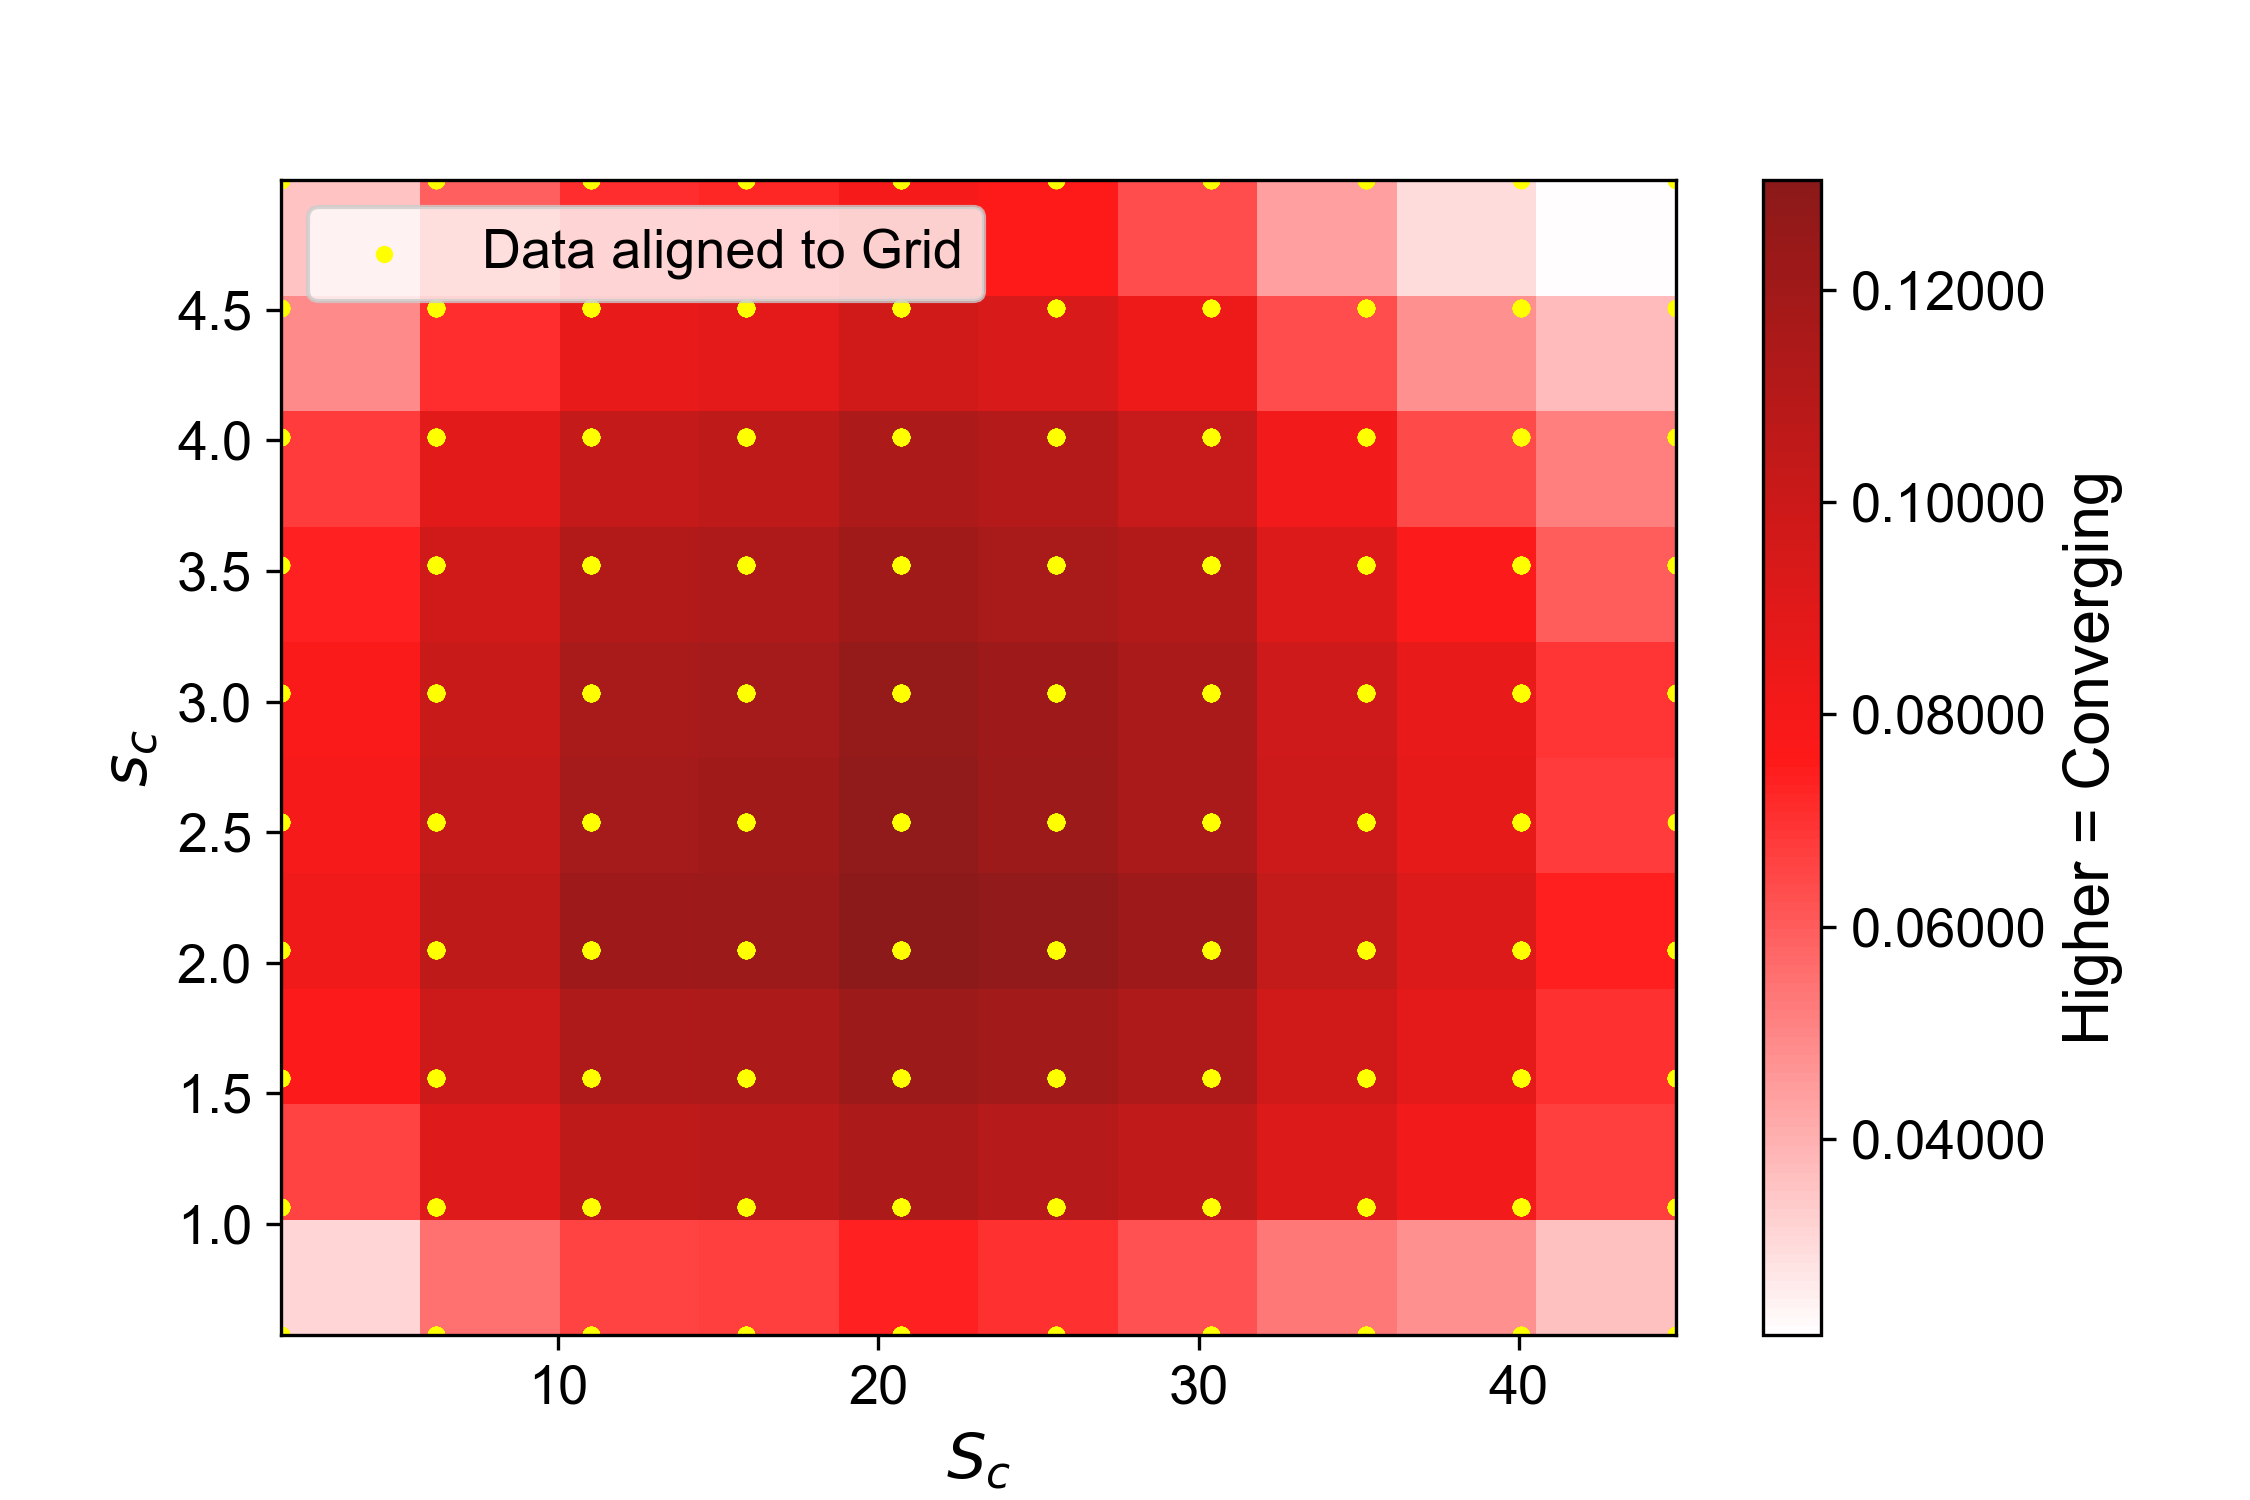
\includegraphics[width=0.32\textwidth]{figures/convergence/pairwise_projections_19.png} &
			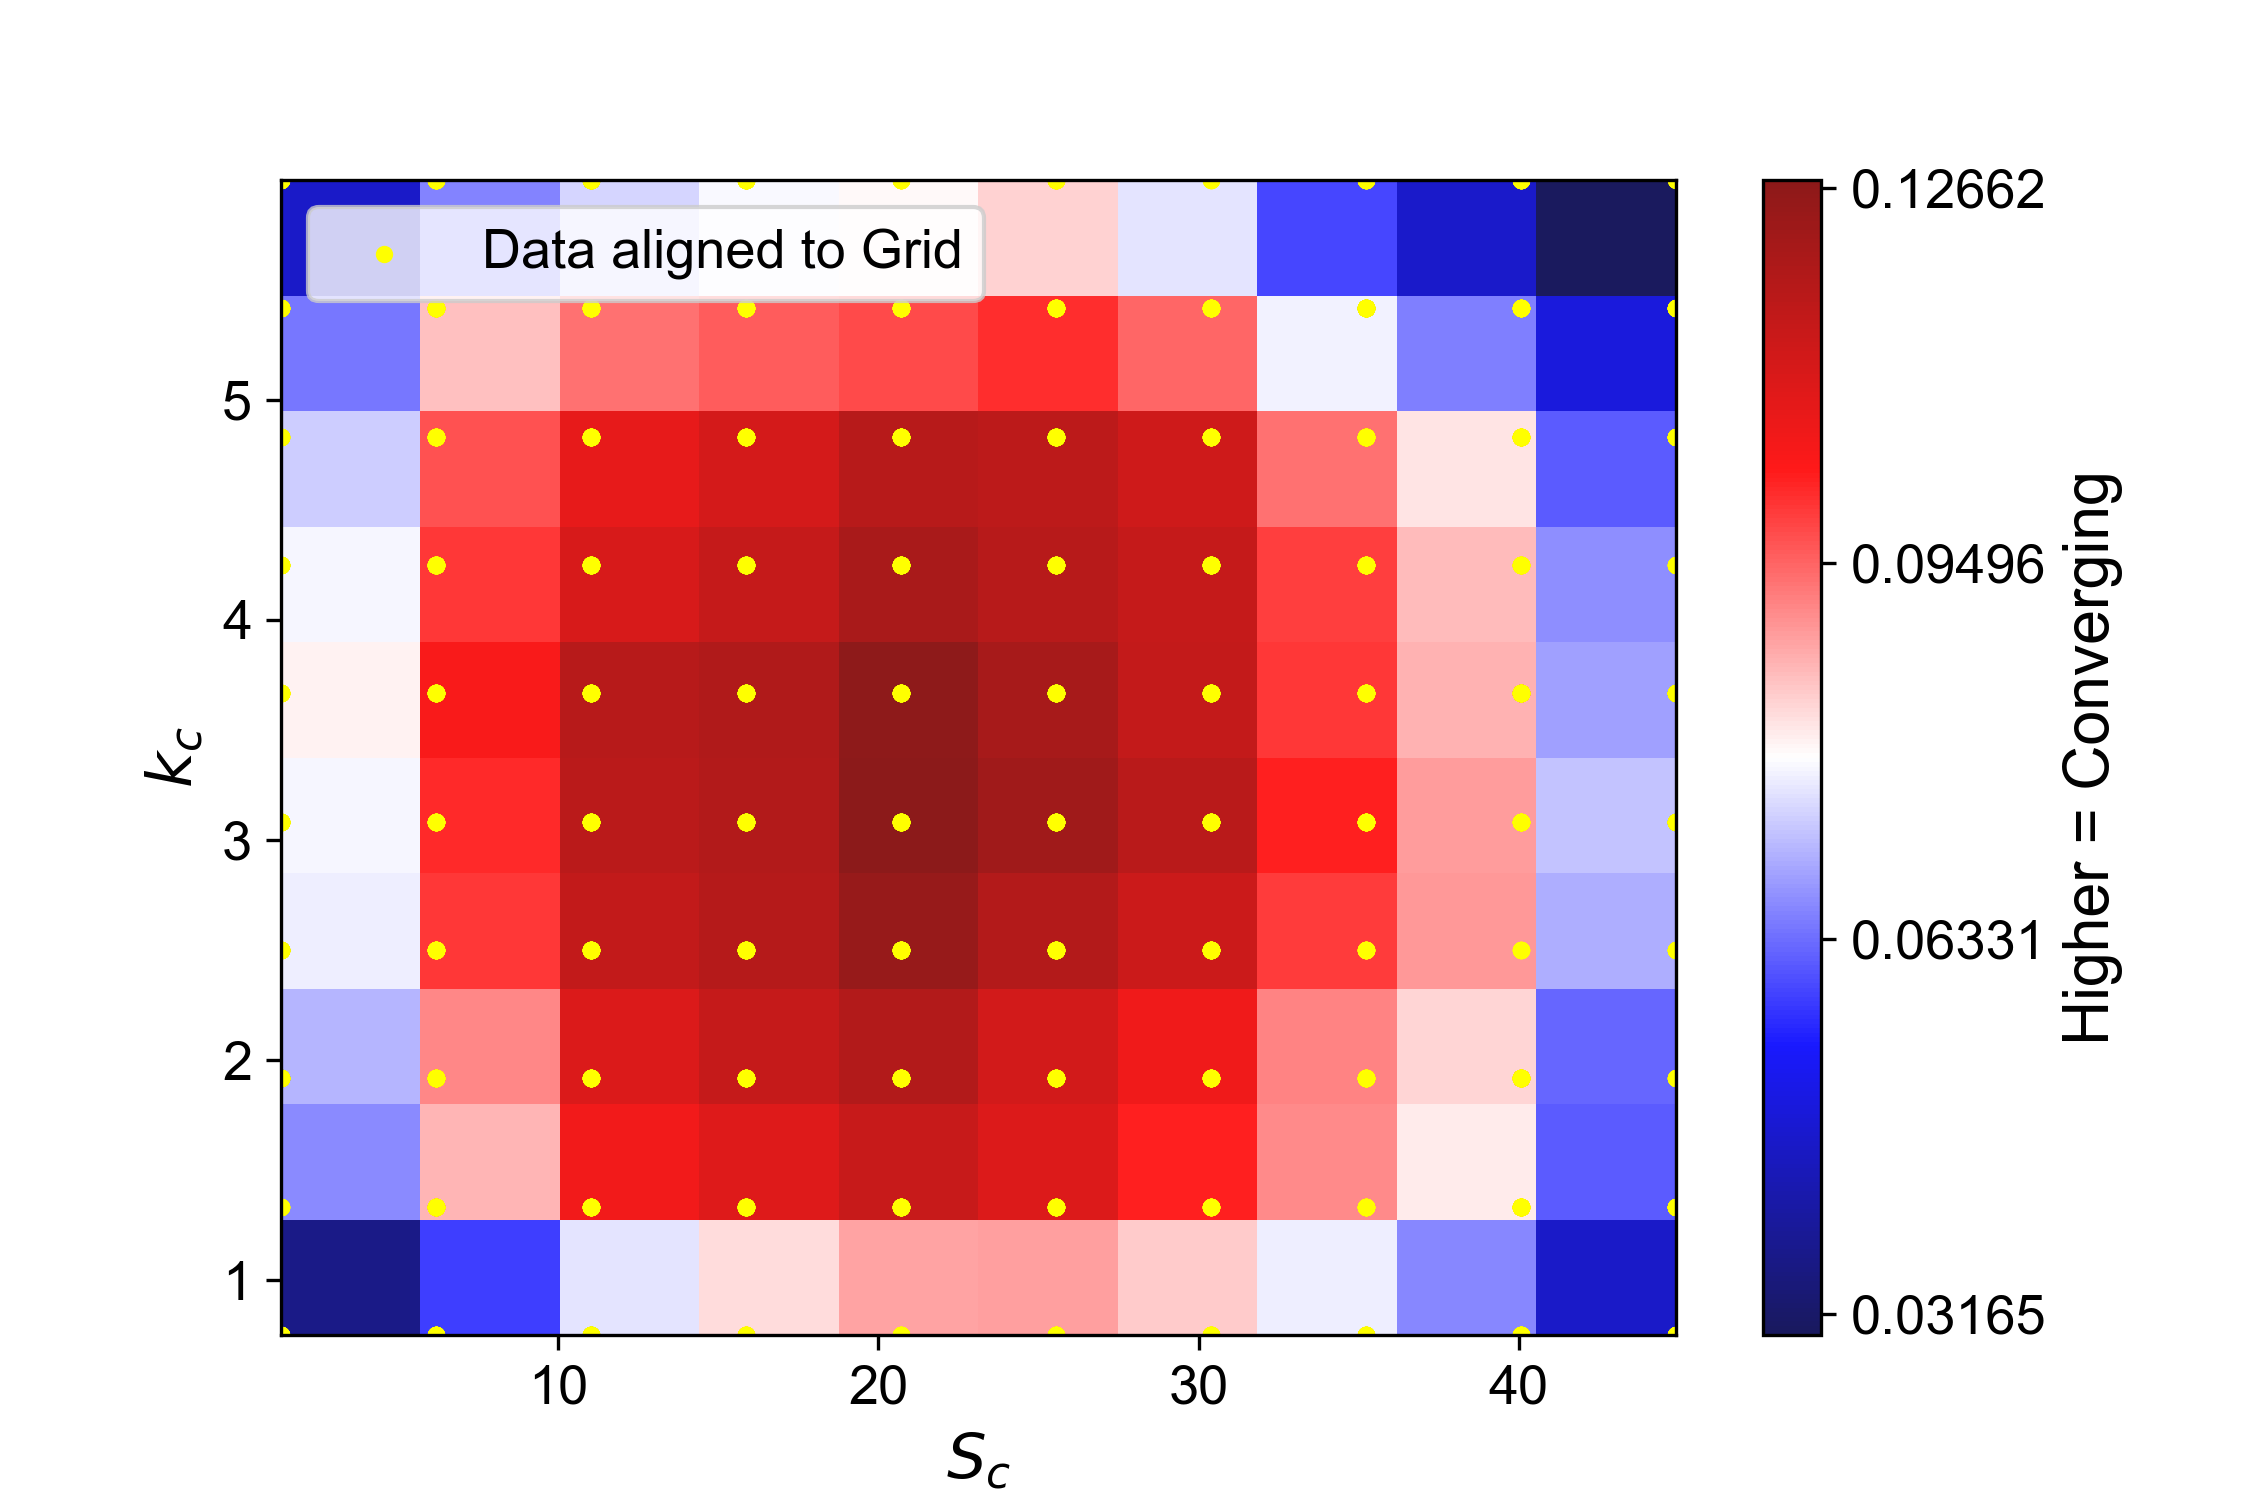
\includegraphics[width=0.32\textwidth]{figures/convergence/pairwise_projections_20.png} &
			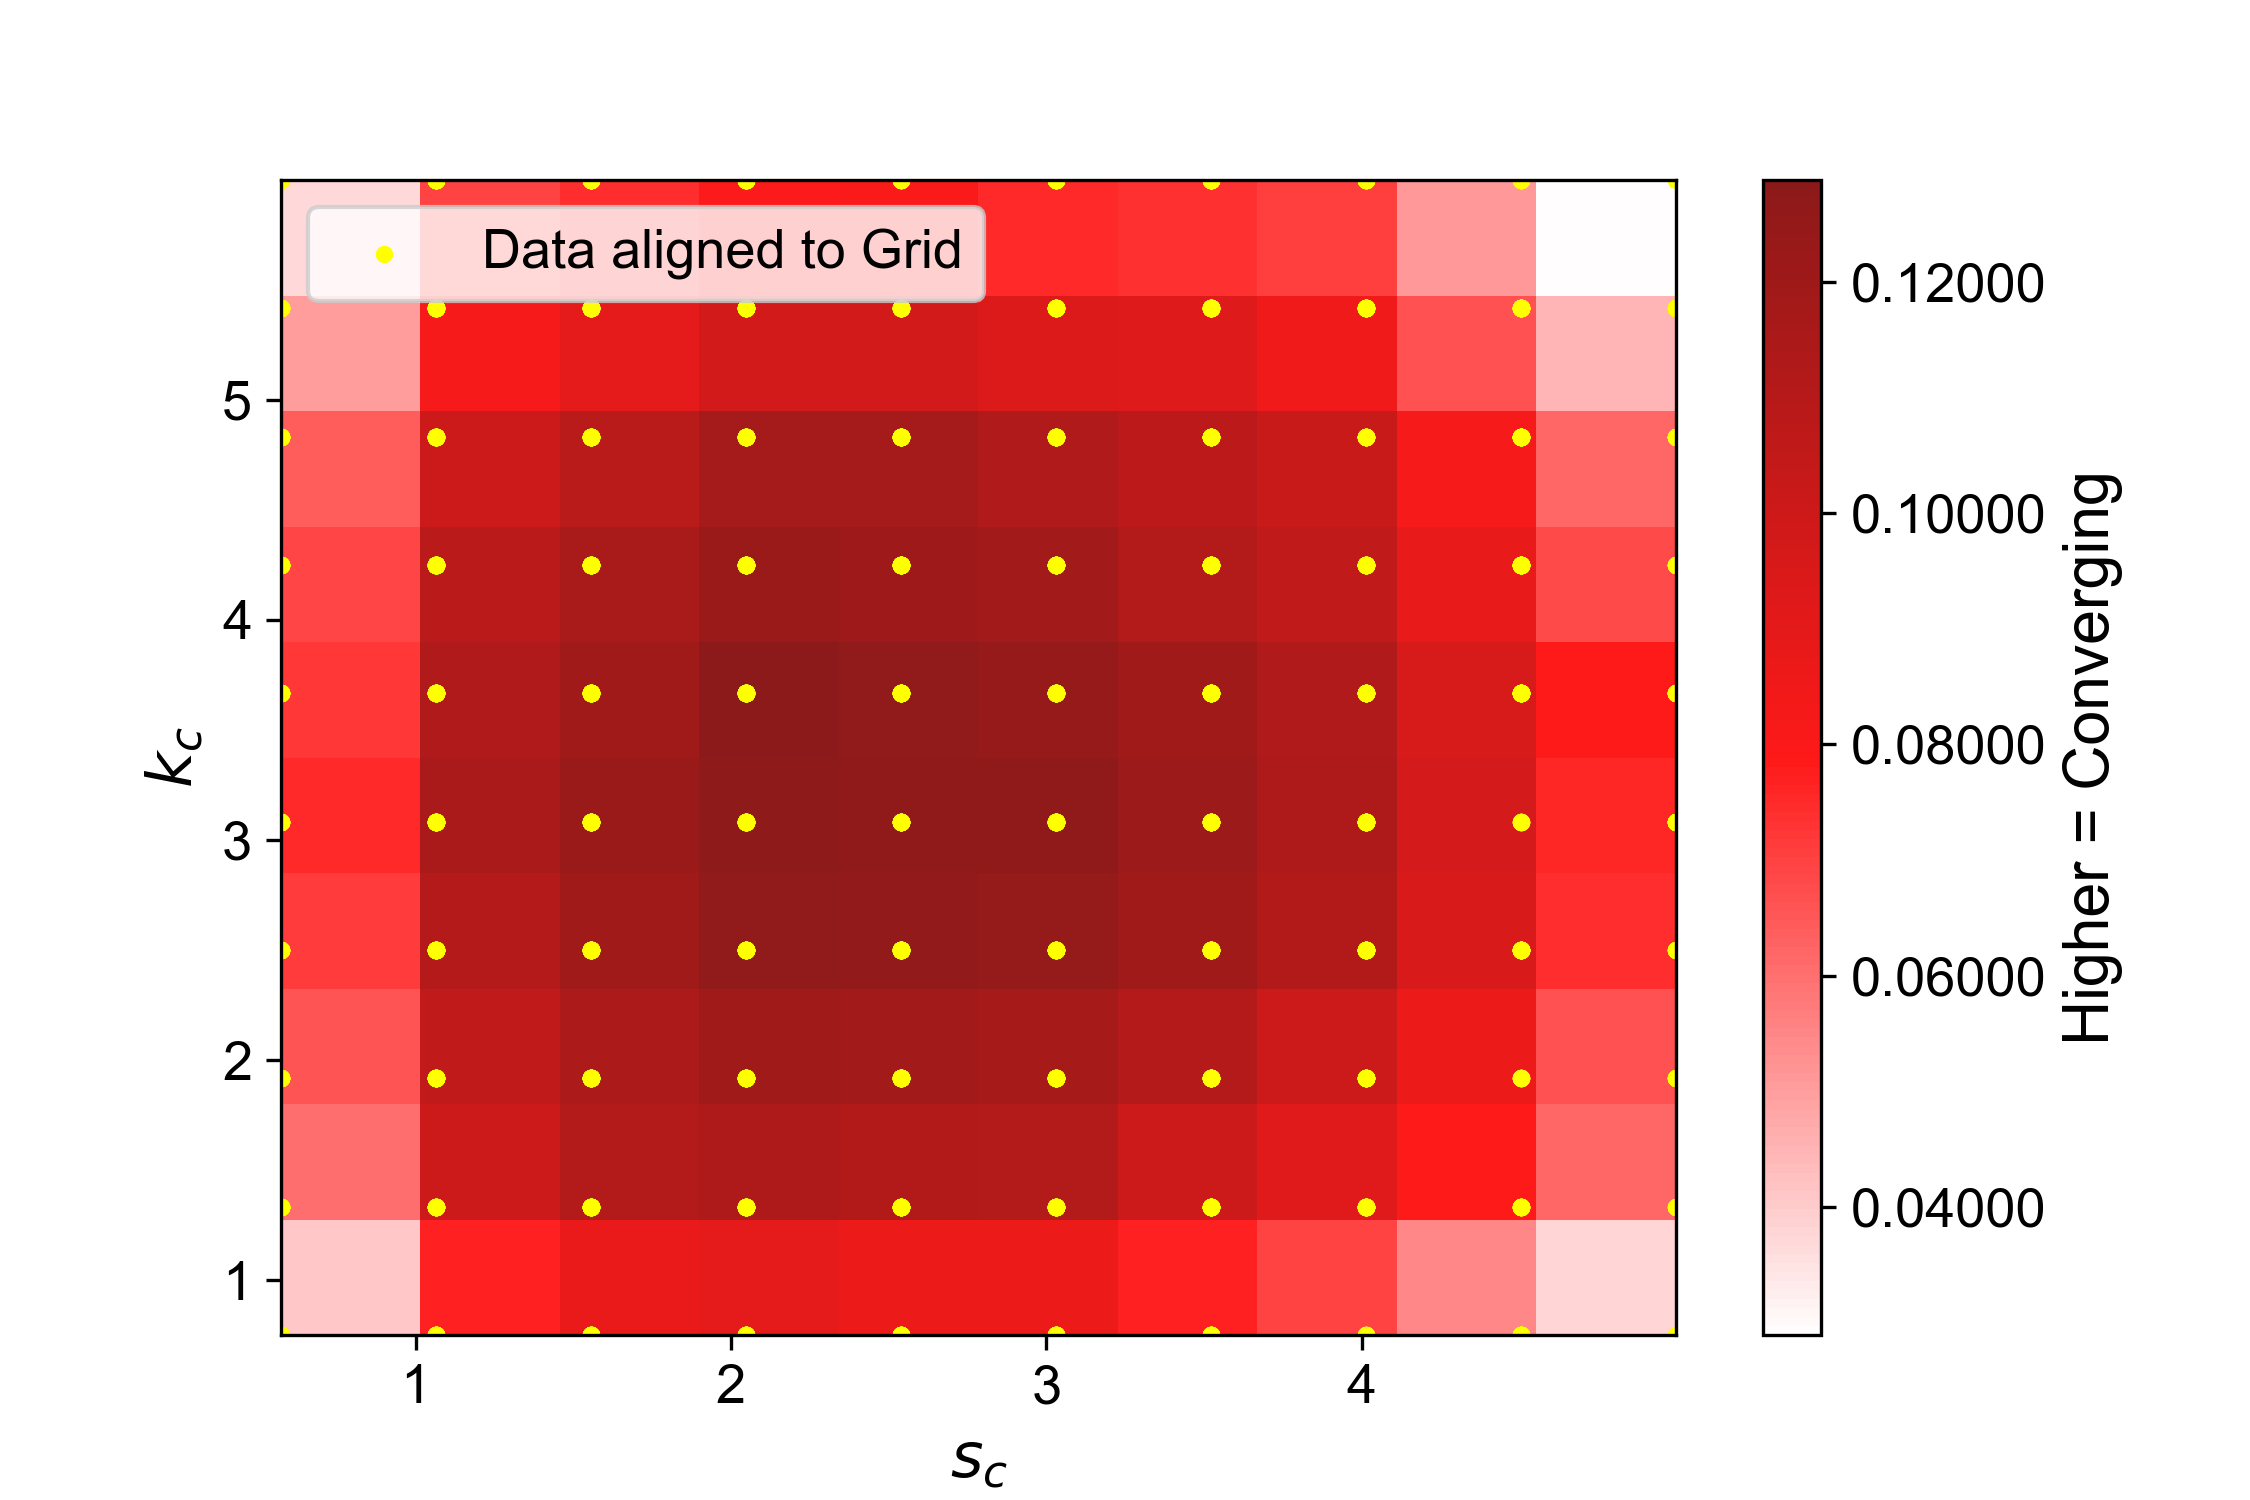
\includegraphics[width=0.32\textwidth]{figures/convergence/pairwise_projections_21.png} 
			% Continue until 21 images
		\end{tabular}
		\caption{Pairwise projections of the material model parameters.}
		\label{fig:pairwise_projections}
	\end{figure}
	
	\noindent
	\begin{minipage}{\textwidth}
		The creep curves sampled from the active learning are shown in the figure~\ref{fig:creep_curves_AL_lagamine}. Only 980 curves converged when the model parameters were input to Lagamine solver.
		
		\vspace{1em}
		\begin{center}
			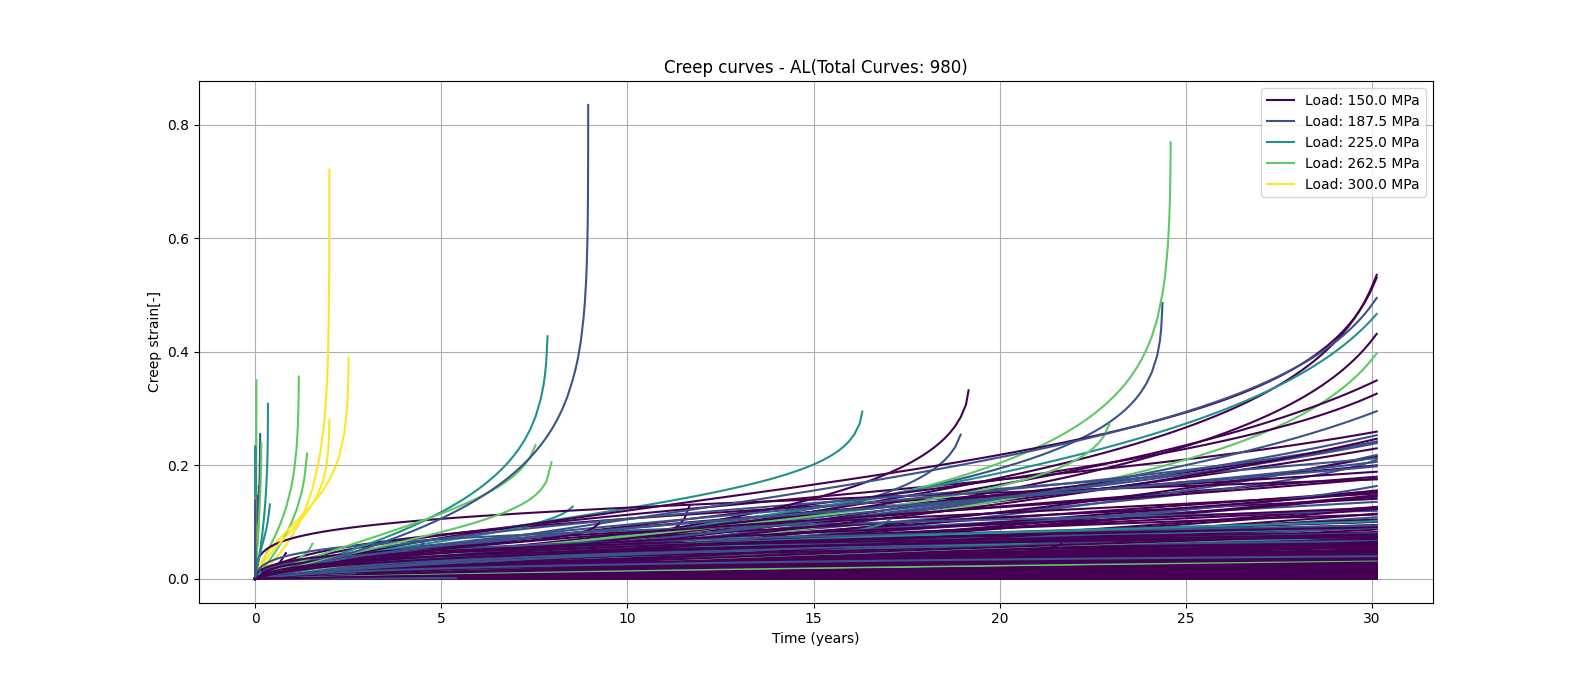
\includegraphics[width=0.9\textwidth]{figures/creep_curves_AL_lagamine.png}
			\captionof{figure}{Creep curves sampled from AL.}
			\label{fig:creep_curves_AL_lagamine}
		\end{center}
	\end{minipage}
	
	\begin{table}[H]
		\centering
		\caption{Summary of Active Learning Results}
		\label{tab:al_summary}
		\begin{tabular}{lc}
			\toprule
			\textbf{Description} & \textbf{Value} \\
			\midrule
			Total queries attempted & 2000 \\
			Converged simulations & 980 \\
			Initial training samples & 100 \\
			Model used in loop & MLP (for $\theta$ projection) \\
			Sampling strategy & Differential Evolution + Feasibility Filter \\
			\bottomrule
		\end{tabular}
	\end{table}
	
	\clearpage
	
	\ifstandalone
		\printglossary
		\printbibliography[heading=bibintoc]
	\fi
	
\end{document}
